\chapter{\texorpdfstring{\ds and \dpl signal extraction}{Ds+ and D+ signal extraction}}\label{chap:RY}

The main ingredient for the evaluation of the \ds/\dpl production-yield ratio are the \ds- and \dpl-meson raw yields, i.e., the number of reconstructed and selected \ds and \dpl mesons. Due to the vast amount of combinatorial background, the extraction of the raw yields through a simple candidate counting method is not feasible. Instead, the raw yield is obtained on a statistical basis by fitting the invariant-mass distribution of the \ds- and \dpl-meson candidates passing tight selection criteria. To reduce the combinatorial background and preserve the highest possible efficiency of D-meson selection, Machine Learning algorithms have been employed. The following sections describe the procedure for the extraction of the raw yield of \ds and \dpl mesons. 


\section{Machine Learning}
The term \emph{Machine Learning} (ML) is a broad and versatile concept, encompassing a wide range of algorithms that grant computers the capacity to learn and adapt without being explicitly programmed to do so~\cite{5392560}. A more comprehensive definition characterises ML as the study of algorithms that enhance their performance at a specific task through the accumulation of experience~\cite{mitchell1997machine}. In recent years, ML techniques have witnessed widespread adoption across diverse fields, with significant impacts realised especially with the emergence of generative models such as GPT~\cite{openai2023gpt4}. ML algorithms have found extensive applications in the high-energy physics field, primarily for the task of distinguishing interesting signals from the vast background present in particle-collision data. Furthermore, these algorithms have been employed as triggers, aiding in the rapid identification of events of interest, and have also been instrumental in event reconstruction. Notably, ML algorithms were used in the discovery of the Higgs boson~\cite{CMS:2012qbp}, one of the most significant achievements in the field of particle physics of the last decades.



\subsection{Supervised learning}
Supervised learning is one of the main branches of machine learning, along with unsupervised and reinforcement learning. Machine learning tasks are usually described in terms of how the machine learning system should process an example, which is a collection of features $\mathbf{x}$ that have been quantitatively measured from some object or event that one wants the machine learning system to process. In the case of supervised learning, each example is coupled with a corresponding label or target, $\mathbf{y}$. The objective of supervised learning is to learn to predict or infer $\mathbf{y}$ based on the associated features, $\mathbf{x}$, assuming that there exists a functional relationship $\mathbf{y} = f(\mathbf{x})$ between the two. The goal of the ML system is to produce an approximation $\widehat{f}(\mathbf{x})$ of the true function $f(\mathbf{x})$ by minimising a given loss function, which quantifies the discrepancy between the predicted and true labels. Supervised learning problems are further segmented into two distinct sub-categories: classification and regression. In the former, the label $\mathbf{y}$ assumes values from a finite and discrete set of categories, often representing distinct classes or groups. In the latter, the label $\mathbf{y}$ takes the form of one or more continuous variables, necessitating the learning system to deduce a continuous function or mapping between $\mathbf{x}$ and $\mathbf{y}$.

The usage of ML algorithms in classification problems, such as the one presented in this Thesis, allows for the definition of multi-dimensional non-linear decision boundaries, which are not available with traditional selection methods based on linear selections on some cut variables. This is particularly important as it provides more efficient selections and a larger purity of the selected data sample.

The application of a supervised learning algorithm to a dataset involves the following steps: i) the model's hyperparameters are optimised through reduced training phases; ii) the optimised model is trained on a set of labelled data, i.e., the value of $\mathbf{y}$ is known for each example in the training set; iii) the model is tested on a separate set of labelled data, known as the test set, to evaluate its performance; iv) the model is then used to make predictions on new, unseen data.

\subsubsection{Hyperparameters tuning}
Before the training phase, hyperparameter tuning is performed to optimise the model's performance. \emph{Hyperparameters} are parameters that are not learned during the training process, but rather define the model's architecture and the training process itself. Hyperparameter tuning is usually performed through a grid search, random search, or with a more efficient bayesian optimisation~\cite{frazier2018tutorial,snoek2012practical,mockus2005bayesian}. Several combinations of hyperparameters are tested on a dedicated labelled dataset: the validation set. Models with different hyperparameter sets are trained with a reduced training phase, and the one yielding the best performance is then selected for a full training phase.

\subsubsection{Training}
During the training process, the model learns (i.e., adjusts its internal parameters) to map the input features $\mathbf{x}$ to the corresponding labels $\mathbf{y}$ by minimizing a given loss function. Typically used loss functions include the Mean Squared Error (MSE) for regression tasks and the Cross-Entropy loss~\cite{mao2023cross} for classification tasks. The loss function is minimised through an optimisation algorithm, usually stochastic gradient descent~\cite{10.1214/aoms/1177729392}, which iteratively updates the model parameters to reduce the loss. Since an over-optimisation of the model on the training data can lead to poor generalisation on unseen data (the model is said to be \emph{overfitting}), a regularisation term is often added to the loss function to penalise overly complex models. The training process continues until the model reaches a satisfactory level of performance on the training data, or until its performance does not improve further. 

\subsubsection{Cross-validation}

With the strategy defined above to optimise the hyperparameters and train the model, the training dataset is divided into two subsets: the validation set and the training set, which are used for hyperparameter tuning and training, respectively. When small datasets are involved, this division can lead to a suboptimal model, as the model's performance can be highly dependent on the specific examples in the training and validation sets. Furthermore, this approach limits the amount of data available for training the model, which can lead to poor generalisation. To mitigate this issue, cross-validation~\cite{stone1974cross} is often employed. This term refers to a set of techniques that allow for a more robust estimate of the model's generalisation performance by using the entire dataset for training and validation. The most common cross-validation technique is the $k$-fold cross-validation. It consists in dividing the training sample into $k$ subsets of equal size, called \emph{folds}. Then, the ML algorithm is trained $k$ times, each time using $k-1$ folds as training set, while the remaining fold is used as validation set. The model's performance is then averaged over the $k$ folds to obtain a more robust estimate of this quantity. This operation is repeated for each hyperparameter configuration to be considered. The hyperparameter configuration minimising the loss function or other metrics used to evaluate the model's performance is then chosen as the optimal configuration.


\subsubsection{Testing}
After the model has been trained, its performance is evaluated on a dataset that was not used during the training process, known as the test set. Like the training and validation sets, also the test set contains labelled examples, but the labels are not provided to the model. While the model is optimised to minimise the loss function during the training phase, the test set is used to estimate the model's generalisation error, i.e., how well the model performs on unseen data. The model's performance is evaluated using metrics that are specific to the task at hand, such as accuracy for classification tasks, or Mean Squared Error (MSE) for regression tasks. Once the model achieves satisfactory performance on the test set, it is ready to be used for making predictions on unlabelled data.


\section{\texorpdfstring{\ds and \dpl selection using Machine Learning}{Ds+ and D+ selection using Machine Learning}}

The task of extracting \ds- and \dpl-meson signals from the vast combinatorial background is a challenging one, due to the large amount of background compared to signal. It is however an excellent example of classification problem, and ML algorithms can therefore be exploited to enhance the efficiency of the selection. 

\subsection{Data preparation}\label{sec:ml_data_preparation}
In order to train a ML model, a labelled dataset with a well-defined set of features is required. The dataset used for training the ML algorithms employed in this Thesis is composed of a number of signal and background examples. To obtain a pure sample of signal candidates, Monte Carlo (MC) simulations are used to generate \ds and \dpl mesons and transport their decay products through a simulation of the ALICE apparatus. Proton-proton collisions are simulated using the \textsc{Pythia~8} event generator~\cite{Bierlich:2022pfr} with colour-reconnection Mode~2~\cite{Christiansen:2015yqa}, and the generated particles are propagated through the ALICE detector using the \textsc{Geant4} transport simulation toolkit~\cite{GEANT4:2002zbu}. A dataset enriched of heavy-flavour hadrons is obtained by only selecting (\emph{triggering}) events where at least a $\mathrm{c\overline{c}}$ or $\mathrm{b\overline{b}}$ pair is produced. The produced \ds and \dpl mesons are then forced to decay into the studied decay channels, i.e.: \mbox{$\ds \rightarrow \phi \pi \rightarrow \mathrm{K^+K^-\pi^+}$}, $\ds \rightarrow \mathrm{K^+K^{*0}}\rightarrow \mathrm{K^+K^-\pi^+}$, characterised by the same $\mathrm{K^+K^-\pi^+}$ final state, $\dpl \rightarrow \mathrm{\pi^+K^-\pi^+}$, and $\dpl \rightarrow \phi \pi \rightarrow \mathrm{K^+K^-\pi^+}$. 

%Due to the displaced topology of heavy-flavour decays and the continuous readout employed by the ALICE detector, the selection of events with charm or beauty hadrons produces ``fake'' vertices arising from the association of displaced decay tracks, affecting the reconstruction of heavy-flavour hadrons. To overcome this problem, minimum bias events are generated between charm or beauty enriched ones (\emph{gap-triggered} approach). Studies performed using different gap sizes have shown that a gap of 5 minimum bias events reduces the fake-vertex rate to an acceptable level, while keeping the simulation time reasonable. 

Only prompt and non-prompt \mbox{$\ds \rightarrow \phi \pi \rightarrow \mathrm{K^+K^-\pi^+}$} decays are used to train the model, as \dpl mesons decay into the same final state as \ds mesons, and selections optimised to reconstruct \ds mesons are also effective for \dpl mesons. 

Background candidates are obtained from real data, as MC simulations may not be able to reproduce the complexity of the jet fragmentation and soft processes occurring in the underlying event, therefore limiting the dependence on MC simulations. Background examples are obtained by selecting candidates from a subsample of the full data sample (corresponding to its 3\%) in an invariant-mass region away from both the \ds- and \dpl-meson mass peaks, where $1.7 < M < 1.75$~\gevcc or \mbox{$2.1 < M < 2.15$~\gevcc}, as shown in Fig.~\ref{fig:ml_training_mass}. 
\begin{figure}[htb]
    \centering
    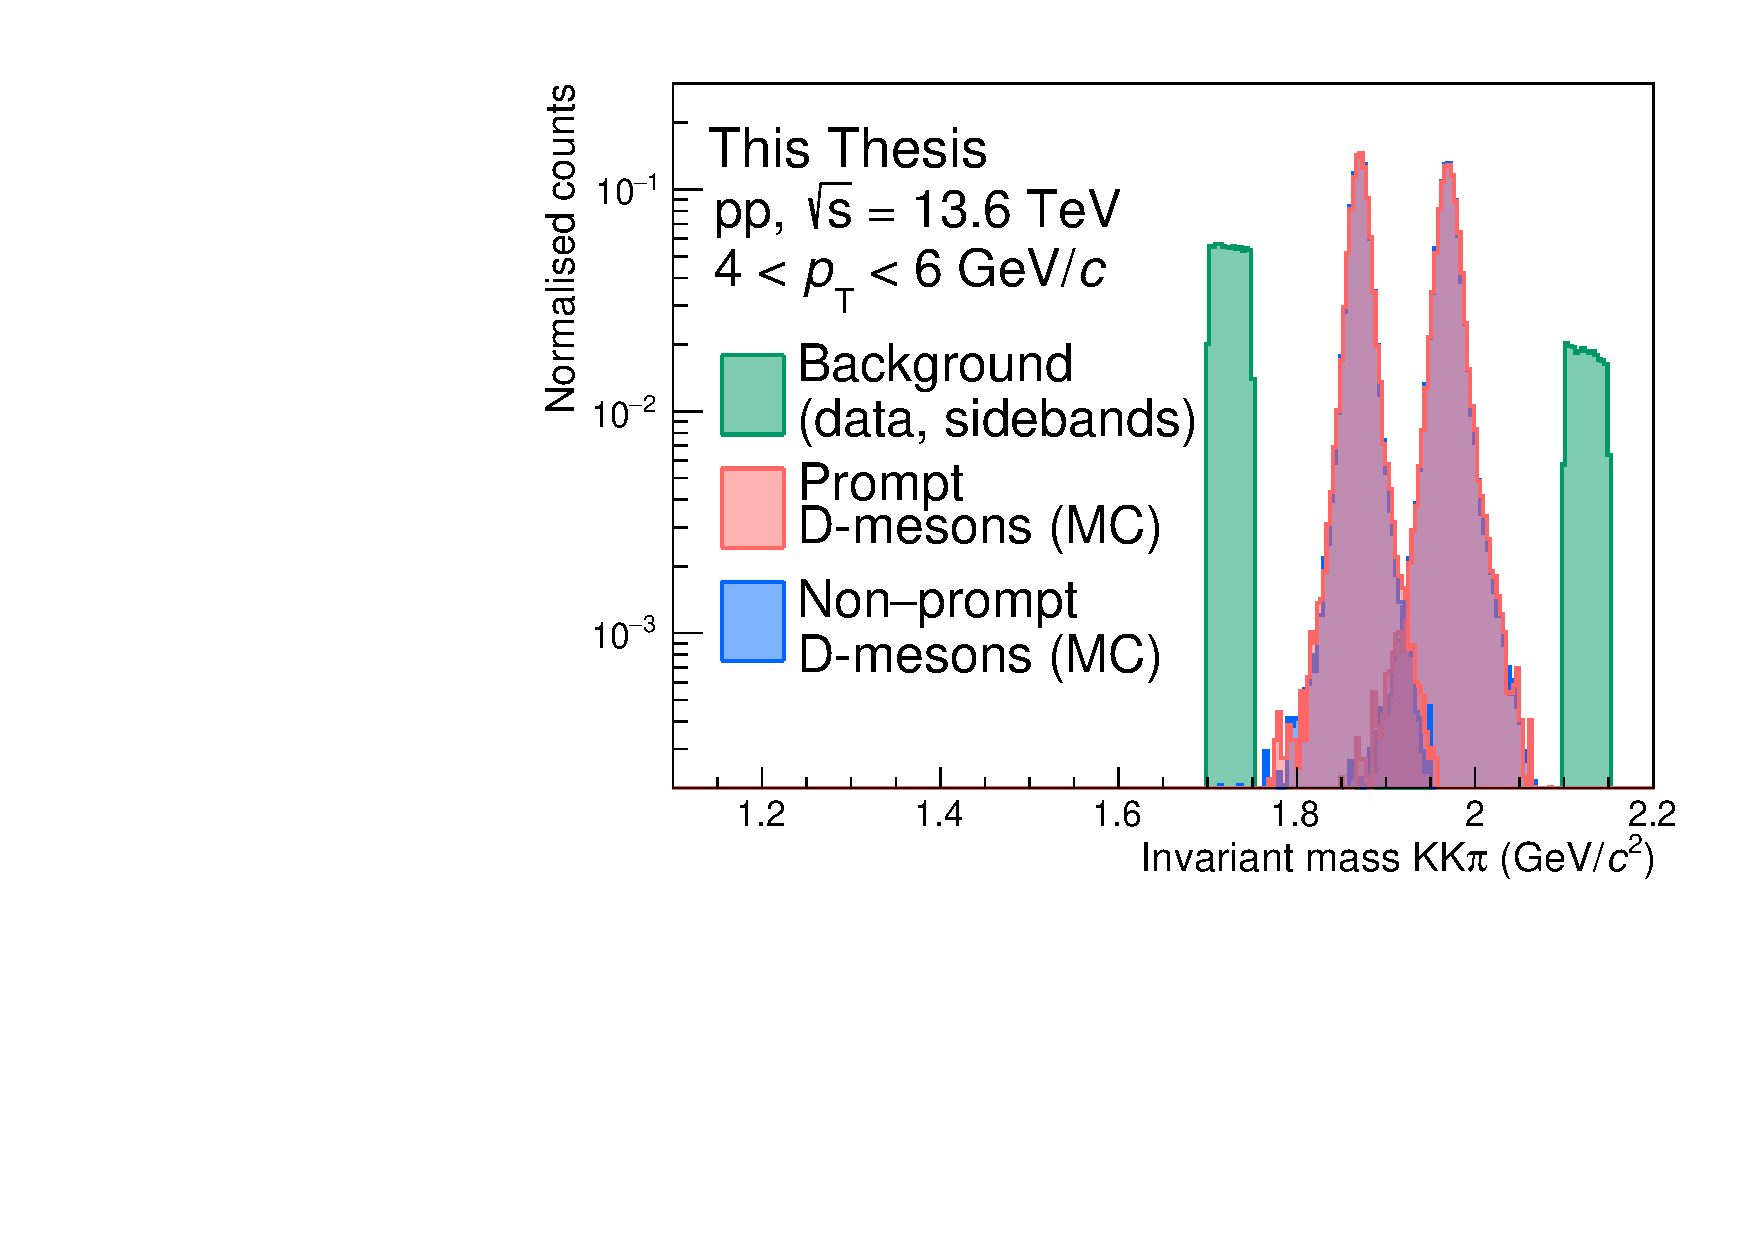
\includegraphics[width=0.7\textwidth]{Figures/Chapter 5/Mass.pdf}
    \caption{Invariant mass distribution of prompt and non-prompt D mesons (red and blue, respectively), taken from MC simulations, and of the background candidates taken from real data used to train the ML model (green) in the \mbox{$4<\pt<6$~\gevc} interval. Background candidates are selected in the \mbox{$1.7 < M < 1.75$~\gevcc} or \mbox{$2.1 < M < 2.15$~\gevcc} invariant-mass interval.}
    \label{fig:ml_training_mass}
\end{figure}

To reduce the amount of combinatorial background in the data samples prior to the application of ML-based selections, some loose selections were applied. These pre-selections are very effective at rejecting the combinatorial background, while preserving the selection efficiency for \ds and \dpl mesons, and are reported in Table~\ref{tab:presel}. These criteria include selections on the invariant mass of the $\mathrm{KK\pi}$ triplet to reduce the number of candidates to those necessary for the invariant mass analysis. To separate signal and background, topological variables such as the decay length $L$ and the cosine of the pointing angle $\cos\theta_\mathrm{p}$, introduced in Sec.~\ref{sec:topologicalSelections}, and PID variables, introduced in Sec.~\ref{sec:PIDselections} were applied. The selection criterion on the $n\sigma_\mathrm{TOF}$ variable is applied only when a TOF cluster is matched to the track, i.e., tracks with no TOF signal are not rejected. In addition, a logical \code{OR} is applied to the conditions on the PID variables, meaning that a candidate is accepted if, for all daughter tracks, at least one of the conditions on the $n\sigma_\mathrm{TOF}$ and $n\sigma_\mathrm{TPC}$ is satisfied. A selection is also applied to the $\chi^2_\mathrm{PCA}$ variable, quantifying the dispersion of the decay tracks around the secondary vertex, normalised to their uncertainty.

\begin{table}[h!]
  \begin{center}
    \caption{Topological and kinematical pre-selections applied to the \ds- and \dpl-mesons candidates. The selection criterion on the $n\sigma_\mathrm{TOF}$ variable is applied only when a TOF cluster is matched to the track, i.e., tracks with no TOF signal are not rejected. In addition, a logical \code{OR} is applied to the conditions on the $n\sigma_\mathrm{TOF}$ and $n\sigma_\mathrm{TPC}$ PID variables, meaning that a candidate is accepted if, for all daughter tracks, at least one of the conditions is satisfied.}
    \vspace*{0.3cm}
    \label{tab:presel}
    \begin{tabular}{c|ccc}
        \toprule
        & \multicolumn{3}{c}{\pt interval~(\gevc)}\\
        \midrule
       Variable & 0.0$-$1.5 & 1.5$-$12 &  12$-$24\\
        \midrule
      $\lvert M - M_\ds^\mathrm{PDG} \rvert~(\mevcc) <$ & 400 & 400 & 400\\
      $\pt(\pi, \mathrm{K})~(\gevc) >$  & 0.3   & 0.4   & 0.4\\
      Decay length (cm) $>$             & 0.02  & 0.02  & 0.03\\
      Normalized decay length XY $>$      &2     & 2     & 2\\
      $\cos\theta_\mathrm{p}>$        & 0.85  & 0.85  & 0.85\\
      $\cos\theta_\mathrm{p}^{xy}>$            & 0.85  & 0.85  & 0.85\\
      $M^{\phi}_\mathrm{inv}$ - $M^{\phi~\mathrm{PDG}}_\mathrm{inv}~(\mevcc) <$ & 20 & 20 & 20\\
      $\chi^2_\mathrm{PCA} < $          & 10    & 10    & 10\\
      $\lvert n\sigma_\mathrm{TPC}\rvert <$                   & 5     & 5     & 5\\
      $\lvert n\sigma_\mathrm{TOF}\rvert <$                   & 5     & 5     & 5\\
      \bottomrule
    \end{tabular}
  \end{center}
\end{table}

Labels are assigned as a numerical value to each candidate, with 0 indicating a background candidate, 1 a prompt \ds meson, and 2 a non-prompt \ds meson.

The dataset is then divided into two different subsamples. The first comprehends 80\% of the data, and is used to train the model, while the remaining 20\% is used to test its performance. In addition, since the D-meson decay topology can significantly differ depending on the \pt of the meson due to different Lorentz boosts, the dataset is divided into several \pt intervals, and the model is trained and tested separately for each of them. To achieve a better performance of the ML models, they are trained in broader \pt intervals than those used for the analysis, to ensure that enough data is available to train a well-performing model. The total number of candidates available for training and testing the model is reported in Table~\ref{tab:training_sample} for the considered \pt intervals.


\begin{table}[tb]
    \begin{center}
    \caption{Number of candidates within the \pt intervals used to train and test the model.}
    \label{tab:training_sample}
    \vspace*{0.3cm}
    \begin{tabular}{c|c}
         \toprule
         \pt (\gevc) & Candidates\\
         \midrule         
         0--1.5     & $\sim 4.6 \times 10^{3}$  \\
         1.5--2     & $\sim 6.1 \times 10^{3}$ \\
         2--3       & $\sim 26  \times 10^{3}$  \\
         3--4       & $\sim 34  \times 10^{3}$  \\
         4--5       & $\sim 31  \times 10^{3}$ \\
         5--6       & $\sim 24  \times 10^{3}$ \\
         6--8       &  $\sim 22   \times 10^{3}$\\
         8--12      & $\sim 10   \times 10^{3}$\\
         12--24     & $\sim 2.6  \times 10^{3}$ \\
         \bottomrule
    \end{tabular}
    \end{center}
\end{table}

\begin{sloppypar}
To produce a balanced dataset, the number of candidates in each class is equalised to the number of examples in the minority class. This is achieved by randomly selecting a subset of the majority classes. The balanced dataset is then used to train the model.
\end{sloppypar}

The choice of features used to separate signal from background is crucial, as they must be able to discriminate between signal and background candidates, and must be chosen in such a way that no bias is introduced in the final result. The variables used to train the model were introduced in Chapter~\ref{chap:reconstruction}, and are a mixture of topological, kinematical, and PID variables. The key idea is to exploit the displaced topology of the D-meson decay, which is a distinctive feature of the signal candidates, the kinematic properties of the D-meson decay, and the PID information of the daughter tracks to discriminate between signal and background candidates. The features used to train the model are reported in Table~\ref{tab:ml_training_vars}. The number in parenthesis after $n\sigma$ indicates the prong identification number. The tracks are ordered based on their charge sign, so that the first and third prongs (prongs 0 and 2) are the like-sign tracks (i.e., their charge sign is the same as that of the D meson), while the second prong (prong 1) is the opposite-sign track.

\begin{table}[tb]
    \begin{center}
    \caption{Candidate features used to train the ML model.}
    \label{tab:ml_training_vars}
    \vspace*{0.3cm}
    \begin{tabular}{c}
         \toprule
         Variable\\
         \midrule         
         Cosine of pointing angle ($\cos\theta_\mathrm{p}$)\\
         Cosine of pointing angle XY ($\cos\theta_\mathrm{p}^{xy}$)\\
         Decay length ($L$)\\
         Decay length XY ($L^{xy}$)\\
         Candidate impact parameter XY ($d^{xy}$)\\
         $\lvert \cos^{3}\theta'(\mathrm K)\rvert$\\
         Prong 0 impact parameter XY ($d_{0}^{xy}$)\\
         Prong 1 impact parameter XY ($d_{1}^{xy}$)\\
         Prong 2 impact parameter XY ($d_{2}^{xy}$)\\
         $n\sigma_\mathrm{comb}^{\pi}(0)$\\         
         $n\sigma_\mathrm{comb}^{\pi}(1)$\\
         $n\sigma_\mathrm{comb}^{\pi}(2)$\\
         $n\sigma_\mathrm{comb}^{\mathrm K}(0)$\\
         $n\sigma_\mathrm{comb}^{\mathrm K}(1)$\\
         $n\sigma_\mathrm{comb}^{\mathrm K}(2)$\\
         \bottomrule
    \end{tabular}
    \end{center}
\end{table}

The invariant mass of the candidate and its \pt are excluded from the model training to prevent any bias in the final results. Including these variables would cause the model to preferentially select candidates within a specific invariant mass range (corresponding to that of \ds and \dpl mesons) or \pt, thereby skewing both candidate selection and the \pt distribution of the final sample, resulting in a biased \pt-differential yield. While it is possible to correct for a \pt-dependent selection using MC simulations, this approach is not taken here to avoid biases from any inaccuracies in the \pt distribution of the D mesons in the simulations. 

Some of the variables used to train the model may be correlated with the invariant mass of the candidate, and the ML may learn to discriminate the signal from the background by exploiting this correlation with the \ds meson mass and transverse momentum, rather than the physical properties of the signal and background. To exclude this possibility, the correlation between the features used to train the model is studied. To quantitatively describe the correlation between the variables, the Pearson correlation coefficient $\rho$ is evaluated for each pair of variables. It is defined as the ratio between the covariance of two variables $x$ and $y$ and the product of their standard deviations, $\rho(x,y) = \mathrm{cov}(x,y)/(\sigma_{x}\sigma_{y})$. It expresses the strength and direction of a linear correlation between two variables, ranging from $\rho = 1$ (perfect positive linear correlation) to $\rho = -1$ (perfect negative linear relationship). $\rho = 0$ indicates the absence of linear correlation.


\begin{sloppypar}
The correlation matrix of the features used to train the model is shown in Fig.~\ref{fig:ml_training_vars} for the prompt \ds, non-prompt \ds and background classes, in the \mbox{$2<\pt<3$~\gevc} interval of D-meson transverse momentum. The correlation with the invariant mass and the transverse momentum is also reported. The Pearson coefficient is encoded in the colour of the cell, with red indicating a positive correlation, blue a negative correlation, and grey no linear correlation. The correlation matrix shows that the variables used to train the model are not linearly correlated with the invariant mass of the candidate, suggesting that a ML model should not modify the invariant-mass distribution of the selected candidates.
\end{sloppypar}

Variables carrying similar physical information, such as those related to the candidate decay length, pointing angle, and impact parameter, are strongly correlated among each other, as expected. Different degrees of correlation between the same variable pairs are observed for the different classes. The ML model can exploit these differences to discriminate between the three classes of candidates.

\begin{figure}[p]
    \centering
    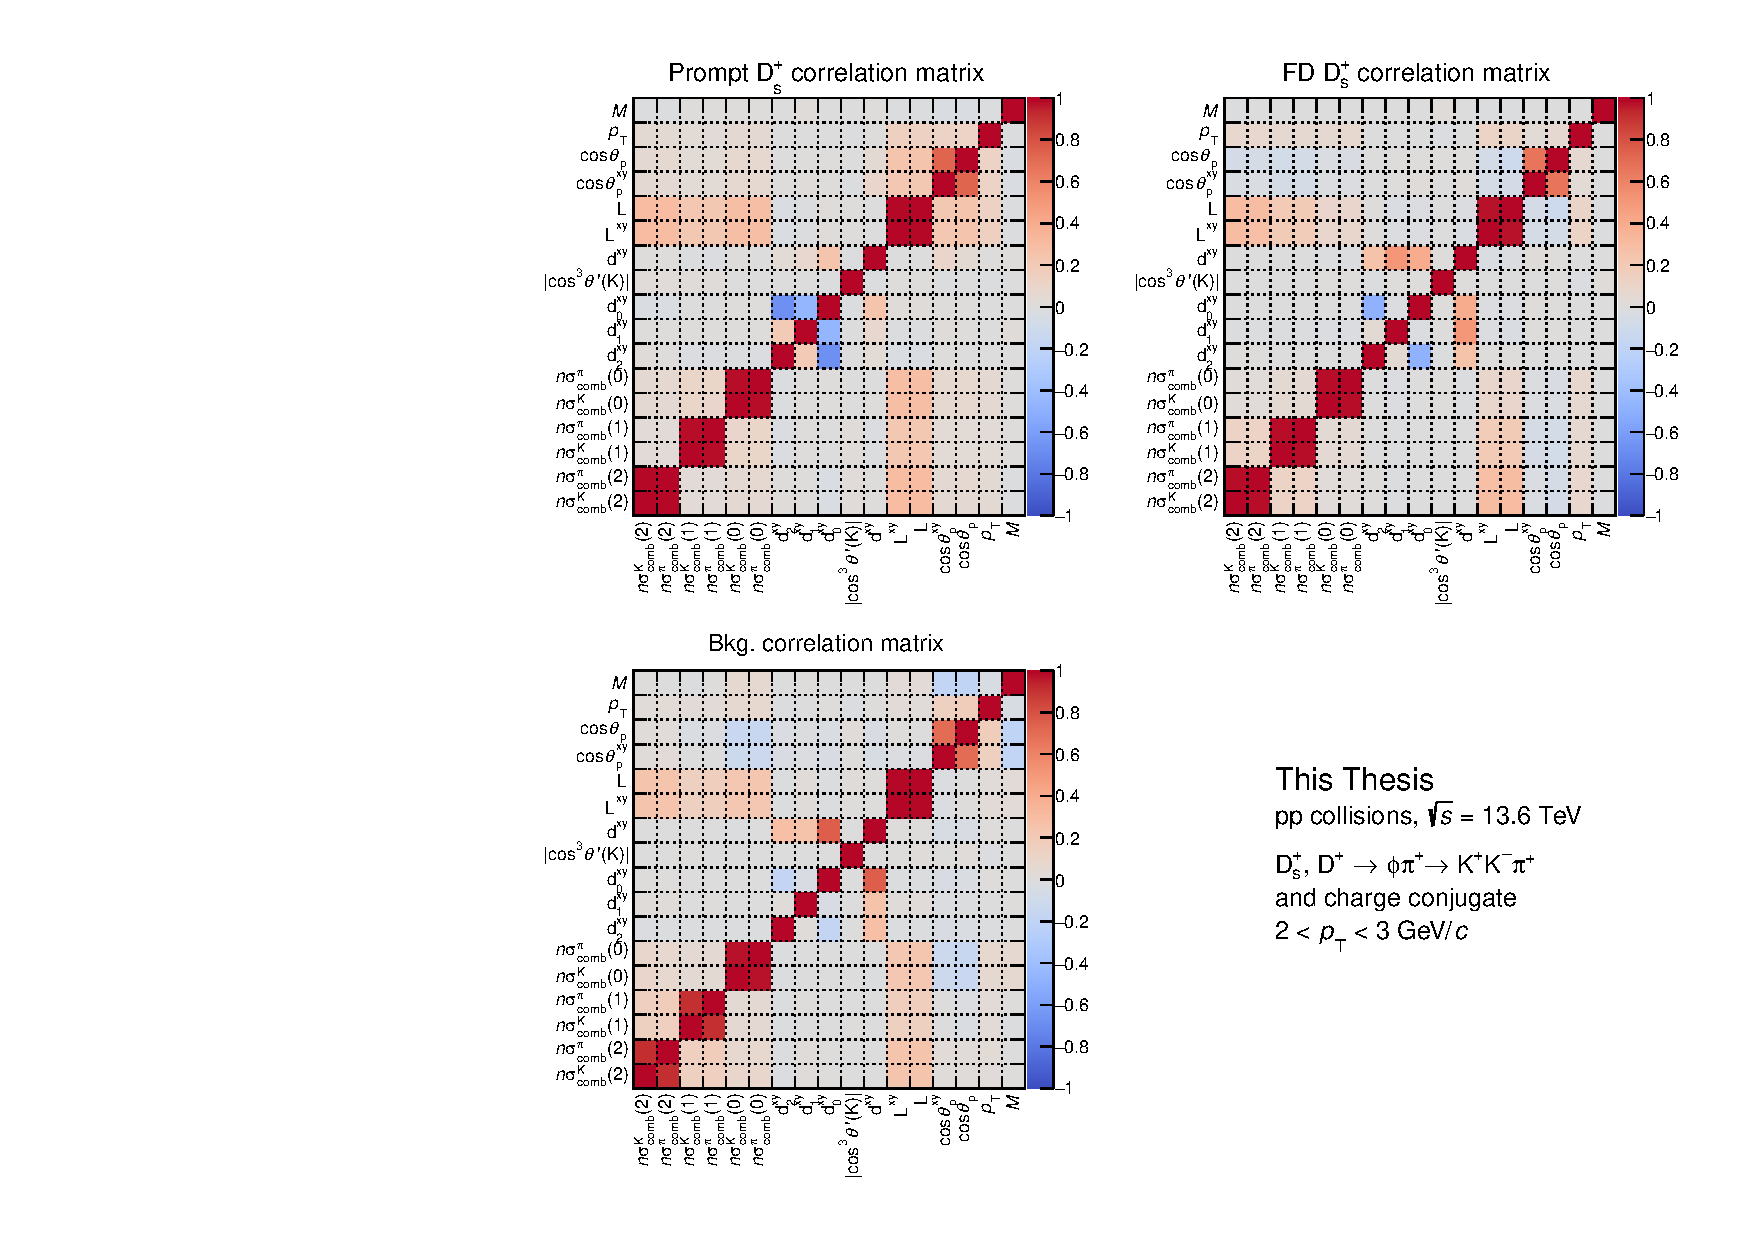
\includegraphics[width=\textwidth]{Figures/Chapter 5/CorrelationMatrix.pdf}
    \caption{Correlation matrices of the features used to train the ML model for prompt \ds (top-left), non-prompt \ds (top-right), and background (bottom-left) candidates in the $2<\pt<3$~\gevc interval. The correlation with the invariant mass and the transverse momentum is also reported. The Pearson coefficient is encoded in the colour of the cell, with red indicating a positive correlation, blue a negative correlation, and grey no linear correlation.}
    \label{fig:ml_training_vars}
\end{figure}

\subsection{Boosted Decision Trees}
Once the training dataset has been composed and the features have been selected, the ML architecture has to be chosen. Several algorithms are available, each with its own strengths and weaknesses. The choice of the algorithm depends on the specific problem to solve, the size of the dataset, and the computational resources available. 

Boosted decision trees~\cite{friedman2001greedy,freund1997decision} (BDTs) are a family of machine learning algorithms employed in different fields, including high-energy physics. Their building blocks are decision trees, which are a versatile type of supervised learning algorithm that can be used for both classification and regression tasks. A decision tree is made of many \emph{nodes}, each containing conditions that split the data into two~\cite{breiman2017classification} or more~\cite{quinlan1986induction} children nodes. The first node of the tree, which receives all the data, is called \emph{root} node, while nodes that do not further split the data are called \emph{leaves}, and contain the output of the tree. The model is trained by considering the Gini index, which measures the impurity of the node:
\begin{equation*}
    G = 1 - \sum_{i=1}^{n} p_{i}^{2}\quad ,
\end{equation*}
where $p_{i}$ is the fraction of samples in the node that belong to the class $i$. The Gini index therefore provides an indication of the quality of the split, with $G=0$ indicating a perfect split. A commonly used algorithm to build \emph{binary} decision trees (i.e., each node contains binary-output conditions, and is split into two children nodes) is the \emph{Classification And Regression Tree} (CART) algorithm~\cite{breiman2017classification}, which recursively splits the dataset into subsets based on a single feature $k$ and a threshold $t_k$ that minimises the impurity of the subsets (weighted by their size). The cost function that the algorithm tries to minimise is given by
\begin{equation*}
    J(k,t_k) = \frac{m_{\mathrm{left}}}{m}G_{\mathrm{left}} + \frac{m_{\mathrm{right}}}{m}G_{\mathrm{right}}\quad ,
\end{equation*}
where $m_{\mathrm{left}}$ and $m_{\mathrm{right}}$ are the number of samples in the left and right nodes, respectively, summing up to the total number of samples $m$, and $G_{\mathrm{left}}$ and $G_{\mathrm{right}}$ are the Gini indices of the left and right nodes. The tree is grown until a stopping criterion is met, such as a maximum depth, a minimum number of samples in a node, or a minimum impurity decrease. These are all hyperparameters that can be tuned to optimise the model's performance.

Given their simplicity, decision trees are fairly easy to interpret, and are often called \emph{white-box} models (in contrast to BDTs and neural networks, where the decision-making process is less transparent, therefore called \emph{black-box} models). An additional strength of decision trees is that they require
very little data preparation, e.g., they do not require feature scaling or centering, making them a very powerful yet simple tool for data analysis. However, they are prone to overfitting, as they can grow to a large depth, capturing the noise in the training data. To mitigate this issue, their depth can be constrained, but this may lead to a model with limited discrimination power. To build a robust model with a good discrimination power, ensemble methods may be used. Several decision trees can be trained, and the final prediction is obtained by combining the outcome of all the trees. 

\subsubsection{XGBoost}
In this work, the Extreme Gradient Boosting~\cite{DBLP:xgboost} (XGBoost) Boosted Decision Trees (BDT) algorithm is used. It has achieved state-of-the-art results in a number of machine learning and data mining challenges (for example in Ref.~\cite{kaggle:higgs}). In addition, this algorithm, which is available as an open-source package, can be easily parallelised on CPUs and GPUs~\cite{mitchell2017accelerating}, thereby reducing the training and application time.

The term \emph{boosting} refers to any ensemble method combining several weak learners into a strong learner. The general idea of most boosting methods is to train many predictors sequentially, each trying to correct its predecessor~\cite{geron2022hands}. The function estimate $\widehat{f}(x)$ is parametrised with an additive functional form:
\begin{equation*}
    \widehat{f}(x) = \sum_{\mathrm{k}=0}^{\mathrm{M}} \widehat{f}_\mathrm{k}(x)\quad ,
\end{equation*}
where M is the number of iterations, $\widehat{f}_\mathrm{0}(x)$ is the initial prediction, and $\widehat{f}_\mathrm{i}(x)$ is the function increment at the $i$-th iteration, also called \emph{boost}. To reduce the loss function, a new weak learner, whose functional form is parametrised as $h(x,\theta)$, can be added to the ensemble:
\begin{equation*}
    \widehat{f}_\mathrm{t}(x) \leftarrow \widehat{f}_{\mathrm{t}-1}(x) + \rho_\mathrm{t} h(x,\theta_\mathrm{t})\quad .
\end{equation*}
$\rho_t$ is the step size, which is optimised for each iteration t, together with the parameters $\theta_\mathrm{t}$ of the weak learner:
\begin{equation*}
    (\rho_\mathrm{t}, \theta_\mathrm{t}) = \arg\min_{\rho,\theta} \sum_{{i}=1}^{\mathrm{N}} L\left(y_i, \widehat{f}_{\mathrm{t}-1}(x_i) + \rho h(x_i,\theta)\right)\quad ,
\end{equation*}
where $L$ is the loss function, and $y_i$ is the true label of the i-th example. Despite having a well-defined set of equations for minimising the loss function, the optimisation of the parameters is not trivial, as the loss function is non-convex and the search space is high-dimensional. Therefore, the optimisation is usually performed using a gradient-based algorithm~\cite{friedman2001greedy,natekin2013gradient}, where $h(x,\theta_\mathrm{t})$ is chosen as the most parallel function to the negative gradient of the loss function with respect to the previous prediction $g_\mathrm{t}(x)$:
\begin{equation*}
    g_\mathrm{t}(x) = E_{\mathbf{y}}\left[ \frac{\partial L(\mathbf{y},\widehat{f}_{\mathrm{t}-1}(x))}{\partial \widehat{f}_{\mathrm{t}-1}(x)} \Bigg{|} x \right] \quad ,
\end{equation*}
where $E_{\mathbf{y}}$ is the expectation over the true labels. The parameters are then optimised by minimising the difference between the negative gradient and the weak learner prediction:
\begin{equation*}
    (\rho_\mathrm{t}, \theta_\mathrm{t}) = \arg\min_{\rho,\theta} \sum_{\mathrm{i}=1}^{\mathrm{N}} \left[-g_\mathrm{t} - \rho h(x_\mathrm{i},\theta)\right]^{2}\quad .
\end{equation*}

Through the iterative addition of weak learners, the loss function is reduced and the model learns the complex patterns of data. The final prediction is obtained by summing the predictions of all the weak learners. In the XGBoost algorithm, the weak learners are decision trees. The output consists of a numerical score for each class, ranging from 0 to 1 and summing up to unity. Each score represents the confidence of the model in the prediction, which can be interpreted as the probability of the example belonging to that class.
\subsection{Tuning the model's hyperparameters}
The XGBoost algorithm has several hyperparameters~\cite{XGBoost_parameters} that can be tuned to optimise the model's performance. The most important hyperparameters are:
\begin{itemize}
    \item \code{eta} or \code{learning\_rate}, which is the step size shrinkage of the gradient descent algorithm. To reduce the risk of overfitting, this factor multiplies the weak-learner prediction ($\rho_\mathrm{t} h(x_\mathrm{i},\theta) \rightarrow \code{eta} \cdot \rho_\mathrm{t} h(x_\mathrm{i},\theta)$), and is usually set to a small value, such as 0.1;
    \item \code{max\_depth}, which is the maximum depth of a single decision tree. A large depth can lead to overfitting, while a small depth can lead to a model with limited discrimination power. Usually, this parameter is set to around 5;
    \item \code{n\_estimators}, which defines the number of trees to train. A large number of weak learners can lead to overfitting, while a small number can lead to a model with limited discrimination power. Usually, the number of weak learners is set to around 1000;
    \item \code{subsample}, which is the fraction of the training data to be used to train each tree at each iteration;
    \item \code{min\_child\_weight}, which is the minimum sum of instance weight needed in a child. It is related to the purity in a node, and it is used to stop the tree growth;
    \item \code{colsample\_bytree}, which is the fraction of features to be used to train each tree at each iteration;
    \item \code{tree\_method}, which defines the algorithm used to build the trees. The \code{hist} option uses an optimised histogram-based algorithm and is usually the fastest.
\end{itemize}

The hyperparameters are optimised using the Optuna framework~\cite{akiba2019optuna}, which proved to be a powerful tool thanks to its state-of-the-art algorithms for sampling the hyperparameter space and for efficiently pruning unpromising trials. The Tree-Structured Parzen Estimator~\cite{bergstra2011algorithms}, is used in this Thesis. It is a Bayesian optimisation algorithm able to explore the hyperparameter space efficiently. The aim of a Bayesian optimisation is to maximise (or minimise, depending on the task) an objective function $f(\mathbf{x})$ by iteratively sampling a bounded hyperparameter space, $\chi$. The algorithm builds a probabilistic model of the objective function, and uses it to decide which hyperparameters to sample next. The model is updated at each iteration, and the hyperparameters that are most likely to improve the model's performance are sampled. The Optuna algorithm is also able to prune unpromising trials, reducing the computational cost of the optimisation. The optimisation is performed using a 5-fold cross-validation, and the hyperparameters that maximise the macro-averaged one-vs-one Receiver Operating Characteristic Area Under the Curve (ROC AUC) metric (described in detail in Sec.~\ref{sec:ml_performance}) are chosen as the optimal configuration. The hyperparameters optimised for the XGBoost model are reported in Table~\ref{tab:ml_hyperparameters} for some representative \pt intervals considered in the model training. An additional hyperparameter, \code{lambda}, which is the $\mathrm{L_2}$ regularisation term, is also optimised. It helps to prevent overfitting by penalising overly complex models. The optimal hyperparameters are then used to train the model on the full training dataset.

\begin{table}[tb!]
    \centering
    \caption{Optimised hyperparameter configuration for some representative \pt intervals considered in the model training.}
    \label{tab:ml_hyperparameters}
    \vspace*{0.3cm}
    \resizebox{\columnwidth}{!}{%
    \begin{tabular}{c|cccccc}
         \toprule
         Hyper-parameter & \multicolumn{6}{c}{$\pt$ interval (\gevc)} \\
         \midrule
            & 0--1.5 & 1.5--2 & 2--3 & 4--5 & 6--8 & 12--24 \\
        \midrule
         \code{max\textunderscore depth} & 3 & 3 & 3 & 3 & 3 & 3\\

         \code{learning\textunderscore rate} & 0.04 & 0.068 & 0.065 & 0.091 & 0.070 & 0.030\\
         
         \code{n\textunderscore estimators} & 473 & 339 & 1352 & 1256 & 1142 & 1188\\ 
         
         \code{min\textunderscore child\textunderscore weight} & 1 & 3 & 10 & 10 & 3 & 5\\
         
         \code{subsample} & 0.87 & 0.95 & 0.84 & 0.95 & 0.81 & 0.88\\
         
         \code{colsample\textunderscore bytree} & 0.91 & 0.98 & 0.90 & 0.96 & 0.88 & 0.89\\

         \code{lambda} & $8.0\times10^{-4}$ & $4.8\times10^{-4}$ & $9.1\times10^{-4}$ &  $3.0\times10^{-4}$ & $1.9\times10^{-4}$ & $6.7\times10^{-4}$\\
         $\code{tree\textunderscore method}$ & $\code{hist}$& $\code{hist}$& $\code{hist}$ & $\code{hist}$ & $\code{hist}$& $\code{hist}$\\
         \bottomrule
    \end{tabular}%
}
\end{table}

\subsection{Evaluation of the model's performance}\label{sec:ml_performance}
After training the model, its performance is evaluated on the test dataset. The model's performance can be assessed using a \emph{confusion matrix}, which summarises the number of examples for a given class (the true label) that are classified by the model as belonging to any of the available classes (the predicted label). A good model should provide a high number of correctly-classified examples (reported on the diagonal of the confusion matrix), and a low number of misclassified examples (off-diagonal elements of the confusion matrix). The confusion matrix also allows an understanding of which classes are more difficult to classify, and which classes are more likely to be confused with each other. An example of a confusion matrix is shown in Fig.~\ref{fig:ml_confusion_matrix} for the XGBoost model trained on the $2<\pt<3$~\gevc interval.

\begin{figure}
    \centering
    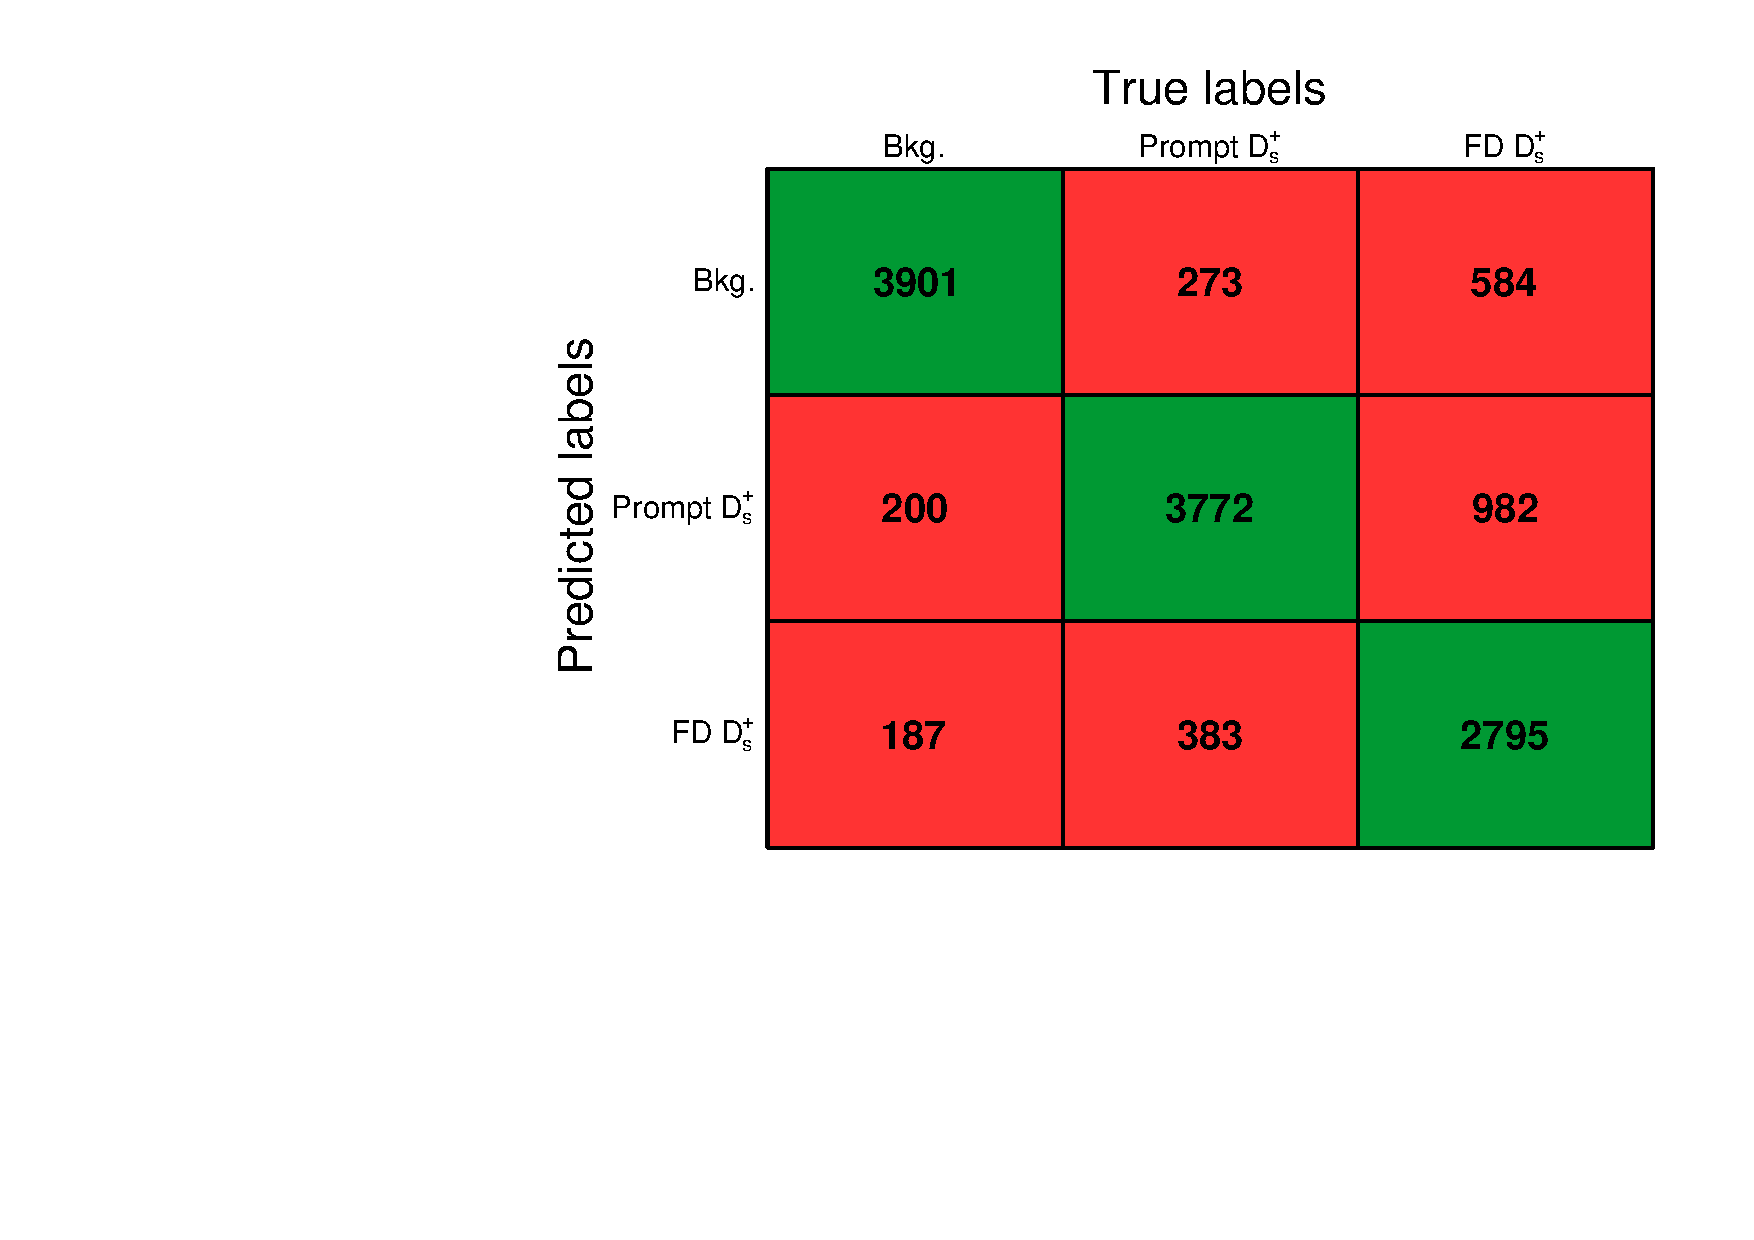
\includegraphics[width=0.7\textwidth]{Figures/Chapter 5/ConfusionMatrix.pdf}
    \caption{Confusion matrix for the BDT model trained in the \mbox{$2<\pt<3$~\gevc} interval. Candidates are classified as the class with the highest score.}
    \label{fig:ml_confusion_matrix}
\end{figure}

Despite providing a lot of information on the model's performance, more concise metrics of the model's performance are usually used, for a more direct comparison between different models. In addition, the confusion matrix provides a threshold-dependent measure of the model's performance, as the classification threshold (i.e., the threshold on the model output that defines the separation between the different classes) can be varied to increase the number of correctly classified signal candidates at the expense of the number of correctly classified background candidates, and vice versa. 

In binary classification tasks, where only two classes are available (a positive and a negative class), several metrics can be defined from the elements of the confusion matrix. The $2\mkern-2mu\times\mkern-2mu2$ confusion matrix contains four entries: the true positives (TP), which are the number of correctly classified positive candidates, the false positives (FP), which are the number of negative candidates being mistakenly classified as positives, and the analogously defined true negatives (TN) and false negatives (FN). One of the most used tools for binary classifiers is the \emph{Receiver Operating Characteristic} (ROC) curve, which represents the true positive rate (TPR) against the false positive rate (FPR) for different threshold values. The TPR is the fraction of correctly classified positive candidates ($\mathrm{TPR = TP/(TP+FN)}$), while the FPR is the fraction of incorrectly classified negative candidates ($\mathrm{FPR = FP/(FP+TN)}$). 

The output of the ML model is a single value ranging from 0 to 1 for a binary classification task, and can be interpreted as the probability of the candidate belonging to the positive class. If positive candidates are selected as those with a score greater than a certain threshold $t$, when $t=0$ all candidates are classified as positive, and both the TPR and FPR will be equal to 1. On the other hand, if $t=1$, no candidate is classified as positive, and the TPR and FPR will both equal 0. Therefore, the different values of $t$ between 0 and 1, which yield different TPR and FPR values, will trace the ROC curve, going from the point (1,1) to (0,0) as $t$ increases. The ROC \emph{Area Under the Curve} (AUC), is used to measure the model's ability to discriminate between positive and negative candidates, for any given threshold. The ROC AUC ranges from 0 to 1. A random classifier has a ROC AUC of 0.5, while a perfect classifier has a ROC AUC of 1. The ROC AUC is a threshold-independent measure of the model's performance, and is often used to compare different models. 

In a multiclass classification task, where more than two classes are available, a generalisation of the ROC curve and the ROC AUC metric is required. In this case, the \emph{One-vs-One} ROC curve~\cite{hand2001simple} can be defined as a plot of the TPR against the FPR for a given pair of classes. The One-vs-One ROC AUC can be averaged to the \emph{macro-averaged} One-vs-One ROC AUC, which is the average of the ROC AUC for each pair of classes and can provide a measurement of the model's ability to discriminate between all the classes. For a classification problem with N classes, there are $\mathrm{N(N-1)}$ possible pairs of ordered classes, and therefore of One-vs-One ROC curves. 


The One-vs-One ROC curves for the model trained on the $2<\pt<3$~\gevc interval are shown in Fig.~\ref{fig:ml_roc_curve}. The ROC AUC is calculated for each class pair, and is reported in the legend. Given that the classification task is a three-class problem, the One-vs-One ROC AUC is calculated for the three possible pairs of classes. Furthermore, despite showing an approximate symmetry around the line $\mathrm{TPR=1-FPR}$, the ROC curve for the A-vs-B pair is not exactly the symmetrical curve of the ROC curve of the B-vs-A pair when more than two classes are considered, due to the different probability of misclassification with the remaining classes. Therefore, two curves are shown for each pair of classes, and present different ROC AUC values. The metric is evaluated on both the training and test sets to test the model's generalisation power. The model's performance is excellent, with a macro-averaged One-vs-One ROC AUC value of 0.965, very close to that of an ideal classifier of 1. In addition, little overfitting is observed, as the ROC AUC values for the training and test sets are similar. The macro-averaged One-vs-One ROC AUC presents similar values in the other \pt intervals, indicating that the model's performance is stable across the studied \pt range. A slight increase in the ROC AUC of a few percent is observed for increasing \pt, due to the more displaced decay topology, which facilitates the separation of the three classes. In the highest \pt intervals the ROC AUC decreases due to the limited number of candidates in the training sample, which can lead to a less performant model. The model is then used to select \ds- and \dpl-meson candidates from the full dataset. 

\begin{figure}[htb]
    \centering
    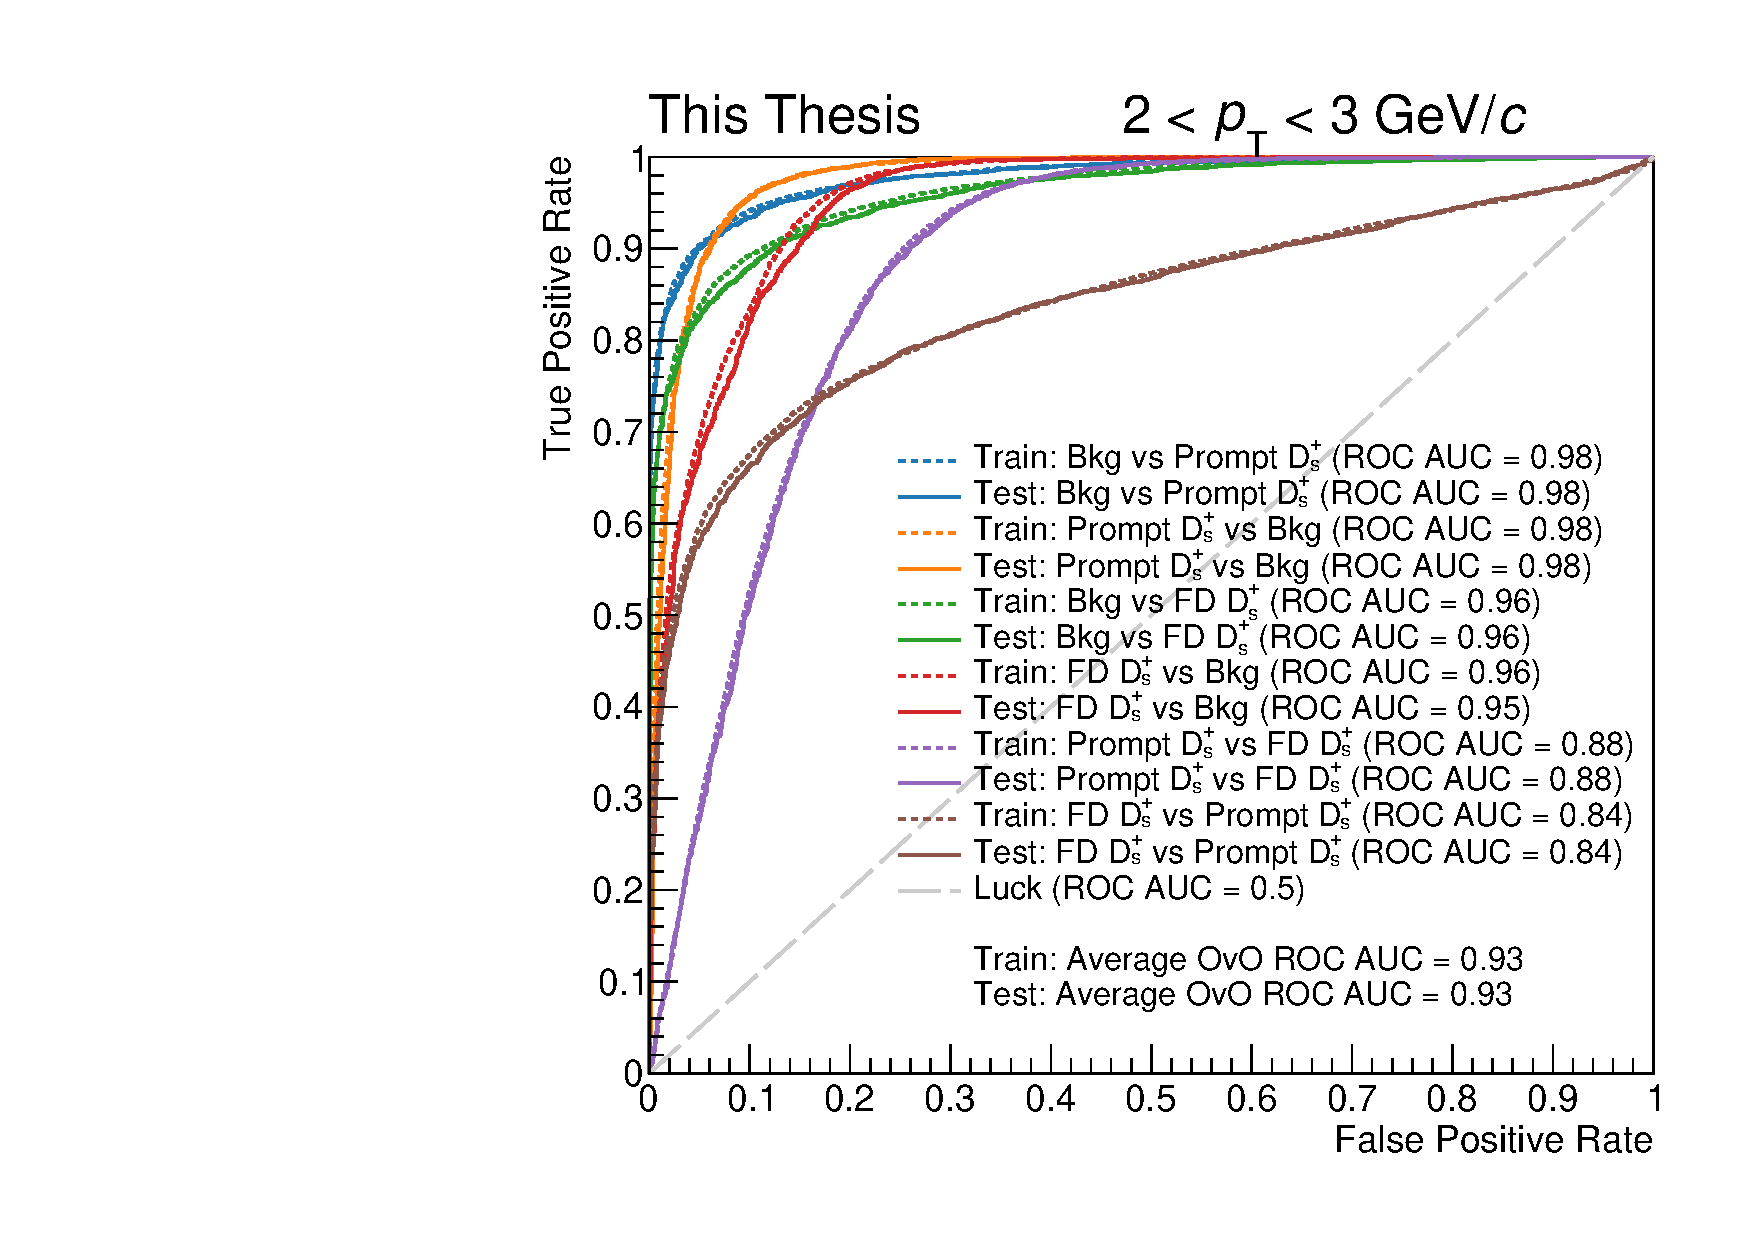
\includegraphics[width=0.7\textwidth]{Figures/Chapter 5/ROC.pdf}
    \caption{ROC curves for the model trained on the $2<\pt<3$~\gevc interval. The One-vs-One ROC AUC metric is calculated for each class pair and reported in the legend.}
    \label{fig:ml_roc_curve}
\end{figure}

\begin{sloppypar}
In addition to the ROC AUC, the model's performance can be evaluated by studying the distribution of the probability of belonging to a given class assigned to labelleled candidates. The score distributions for the model trained on the \mbox{$2<\pt<3$~\gevc} interval are shown in the three panels of Fig.~\ref{fig:ml_score} for the background, prompt \ds-meson, and non-prompt \ds-meson classes. For each class, the score distribution is shown for candidates belonging to the three different classes and to both the training and test sets. The distribution of the true background score provides interesting information on the model's performance. The score distribution for the background candidates peaks at high values, while the score distribution for the signal candidates (both prompt and non-prompt \ds meson) peaks at low values. This highlights that the model has effectively learned to discriminate between signal and background candidates, with good separation power. Furthermore, the score distributions for the training and test sets are fairly similar, indicating that the model generalises well to unseen data. Since non-prompt \ds mesons present a more displaced topology than promptly produced ones, due to the large lifetime of beauty-hadrons, the separation between non-prompt \ds mesons and background is noticeable in the non-prompt \ds-meson score distribution, where the score of true background candidates peaks at zero and the one of non-prompt \ds-meson candidates peaks at one. The distribution of prompt \ds mesons, which have a smaller displacement as compared to non-prompt ones falls in between those of background and non-prompt \ds mesons. Lastly, the separation between the three classes is less pronounced in the prompt \ds-meson score distribution, where the prompt \ds-meson distribution peaks at values significantly lower than one. Similar trends are observed in the other studied \pt intervals. 
\end{sloppypar}

\begin{figure}[p]
    \centering
    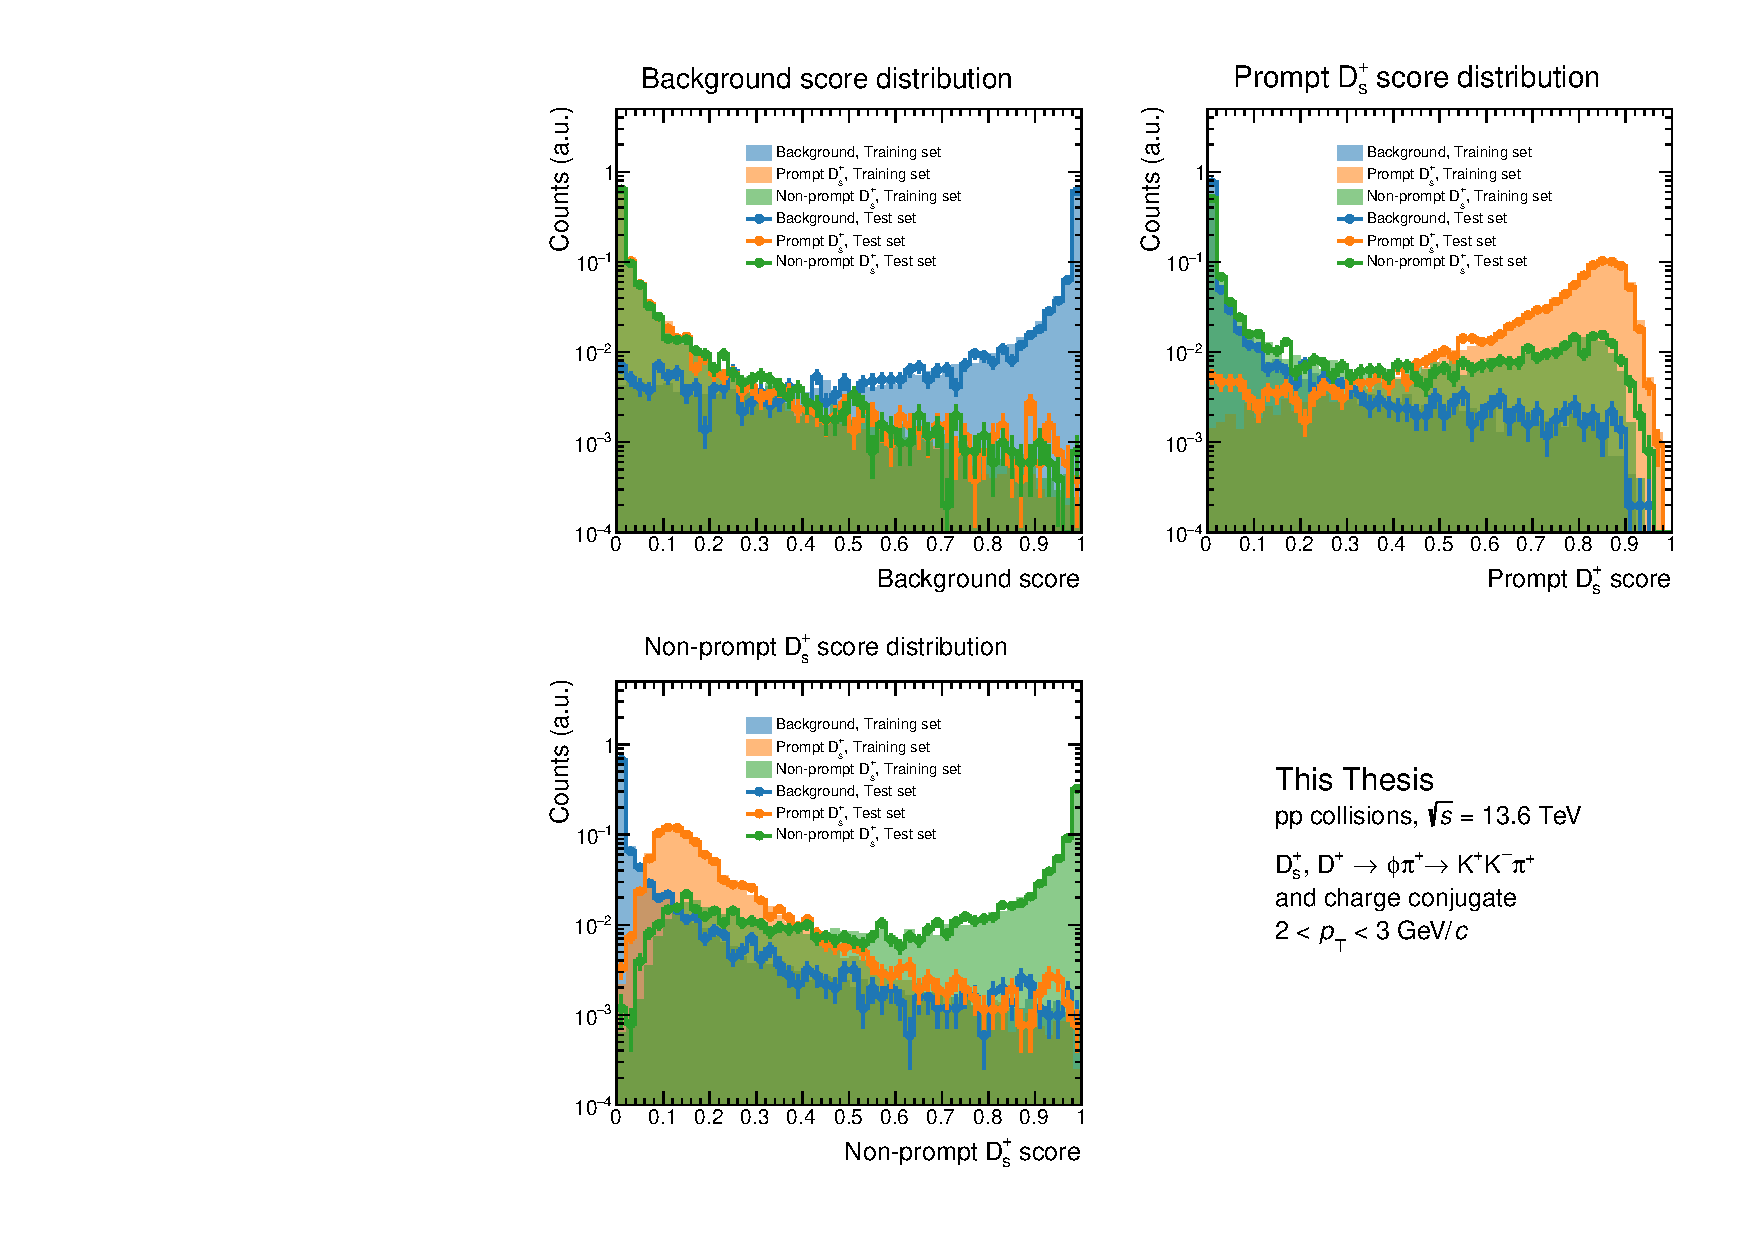
\includegraphics[width=\textwidth]{Figures/Chapter 5/Distributions.pdf}
    \caption{Score distributions for the model trained on the $2<\pt<3$~\gevc interval. The score distributions related to the probability of belonging to the background (top-left panel), prompt \ds-meson (top-right panel), and non-prompt \ds-meson (bottom-left panel) classes are shown. For each class, the score distribution is shown for candidates belonging to the different classes and to both the training (filled area) and test sets (markers).}
    \label{fig:ml_score}
\end{figure}

\subsection{Interpretation of the model's output: Feature importance}
The usage of ML algorithms usually provides a better performance in terms of signal-to-background separation as compared to approaches based on ``rectangular'' cuts, but it also introduces a level of complexity in the selection process. One of the most difficult aspects of using ML models is the interpretation of their output. To understand how the model makes its decisions, the feature importance can be studied. This allows the understanding of which features are more important for the model's decision-making process, and the optimisation of the feature selection. In addition, the feature importance can be used to check whether the model is learning on the correct features in terms of the physics of the problem.

One of the most used algorithms for feature importance studies is the SHapley Additive exPlanations~\cite{lundberg2017unified} (SHAP) algorithm. SHAP is a game-theoretic approach to explain the output of any machine learning model. It is based on the Shapley value~\cite{lipovetsky2001analysis} from cooperative game theory, which requires retraining the model on all feature subsets $\mathcal{S}\subseteq \mathcal{F}$, where $\mathcal{F}$ is the set of all features. An importance value is assigned to each feature i, representing the effect on the model prediction of including that feature. To compute this effect, a model $\widehat{f}_{\mathcal{S}\cup\{i\}}$ is trained with that feature present, and another model $\widehat{f}_\mathcal{S}$ is trained with the feature withheld. Then, predictions from the two
models are compared on the current input \mbox{$\widehat{f}_{\mathcal{S}\cup\{i\}} (x) - \widehat{f}_\mathcal{S}$}. The Shapley values are then computed as the weighted average of all possible differences:
\begin{equation*}
    \phi_\mathrm{i} = \sum_{\mathcal{S}\subseteq \mathcal{F}\setminus\{i\}} \frac{|\mathcal{S}|!(|\mathcal{F}|-|\mathcal{S}|-1)!}{|\mathcal{F}|!} \left[\widehat{f}_{\mathcal{S}\cup\{i\}}(x) - \widehat{f}_\mathcal{S}(x)\right]\quad .
\end{equation*}
Since most models cannot handle arbitrary patterns of missing input values, $\widehat{f} (z_\mathcal{S})$ is approximated with $E[\widehat{f}(z) | z_\mathcal{S}]$, where $z_\mathcal{S}$ is the input missing the features in $\mathcal{S}$. SHAP values therefore explain how to get from the base value $E[\widehat{f}(z)]$, which would be predicted if no features were known, to the output $\widehat{f}(x)$.

A beeswarm-style SHAP feature importance plot for the prompt \ds-meson probability predicted by the model trained in the $2<\pt<3$~\gevc interval is shown in Fig.~\ref{fig:ml_feature_importance}. In this plot, each instance is represented by a single dot on each feature row. The position of the dot along the horizontal axis is determined by the SHAP value of that feature, and the dots ``pile up'' along each feature row, to provide information on the distribution of the SHAP values. The colour of the dot represents the value of the feature, with blue indicating a low value and red a high value. Positive values indicate that the feature is pushing the model's prediction towards the prompt \ds-meson class, while negative values indicate that the model is less likely to classify the candidate as a prompt \ds meson. Feature rows are ordered from top to bottom based on the mean absolute value of the SHAP values for that feature, with the most important features, i.e., those with the highest impact on the model's decision, at the top. The most important features are the cosine of pointing angle $\cos\theta_\mathrm{p}$, the decay length $L$, the decay length in the XY plane $L^{xy}$, the absolute value of the cosine cubed of the K-$\pi$ angle in the KK rest frame $\lvert\cos^3\theta'(\mathrm{K})\rvert$, and the PID information on the prong 1. As discussed in Chapter~\ref{chap:reconstruction}, the first three features are related to the displaced decay topology of \ds mesons, and are therefore expected to be the most important variables in the model decisions. It is also expected that the prong 1 PID information resulted as the most important PID variable, as this is the opposite sign track, which is always a kaon in the considered decay channel. On the contrary, prongs 0 and 2 could be either kaons or pions, resulting in a lower importance of the PID information for these prongs. This check provides a good indication that the model is making decisions based on features that are expected to be relevant for the analysed physics process. 

\begin{figure}[htb]
    \centering
    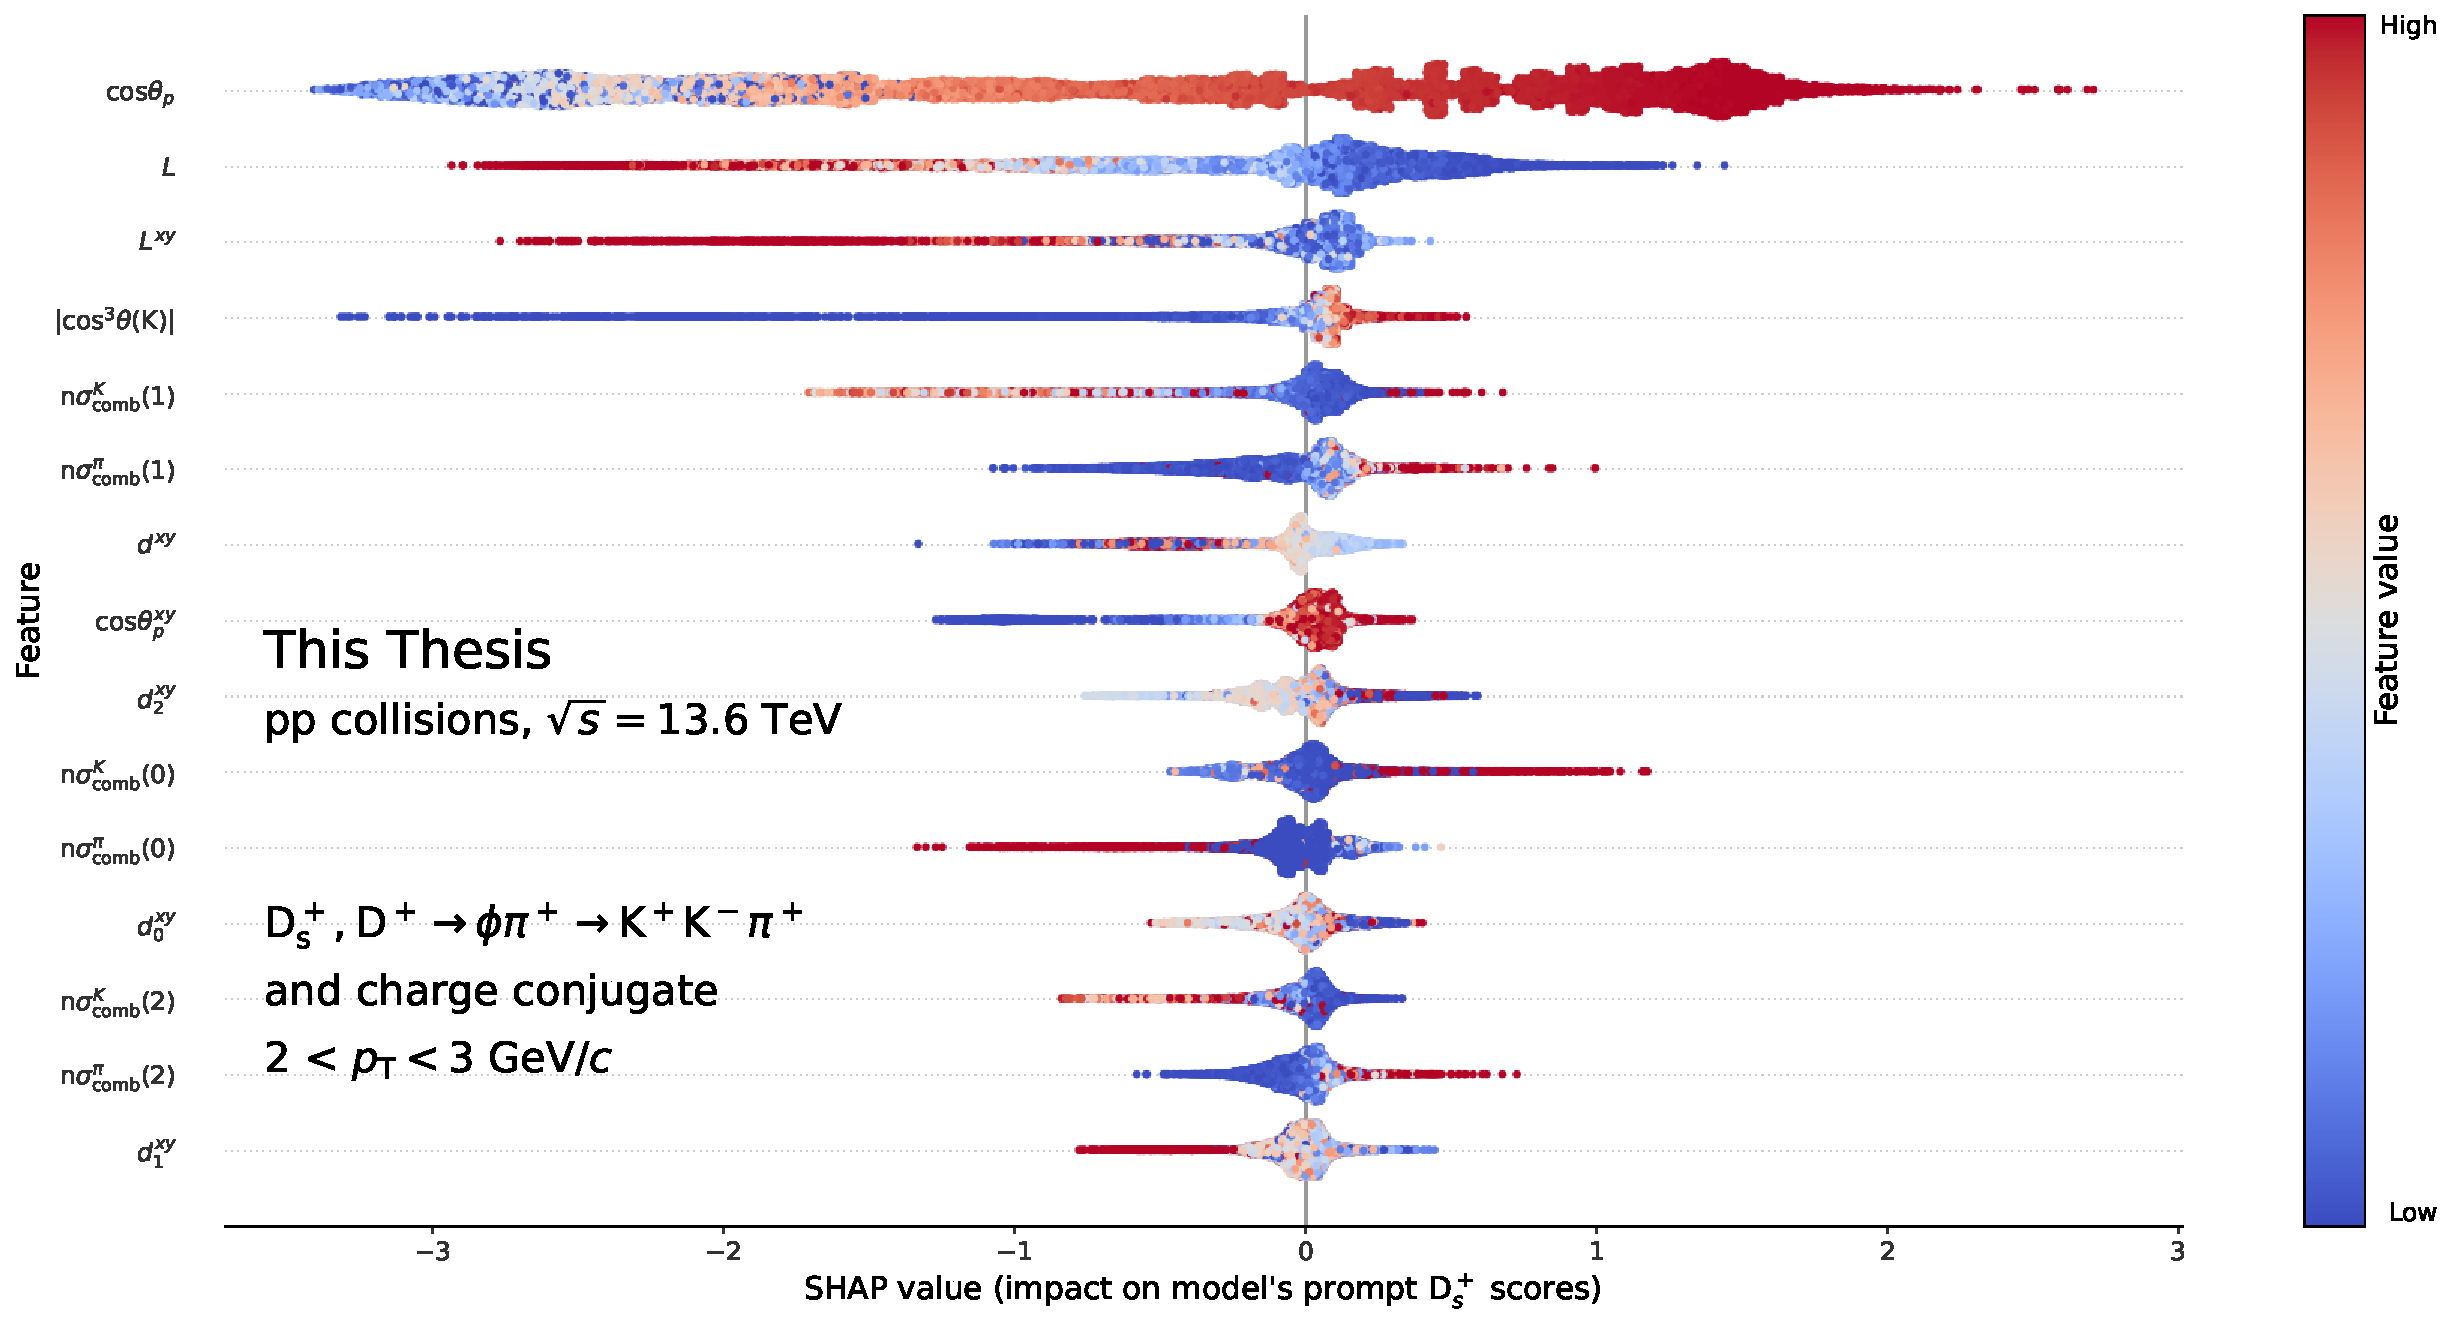
\includegraphics[width=\textwidth]{Figures/Chapter 5/shap.pdf}
    \caption{Beeswarm-style SHAP feature importance plot for the prompt \ds-meson score of the XGBoost model trained on the \mbox{$2<\pt<3$~\gevc} interval.}
    \label{fig:ml_feature_importance}
\end{figure}

For each \pt interval, the SHAP values for the different features employed in the model can be evaluated for the three classes. The overall feature impact on the model's decision can be evaluated by computing the average absolute SHAP value for each feature. The average $|\text{SHAP value}|$ feature importance for the BDT models trained on the $2<\pt<3$~\gevc and $8<\pt<12$~\gevc intervals are shown in Fig.~\ref{fig:ml_feature_importance_average}, providing insights on the evolution of the feature importance across the different \pt intervals. The features are ordered from top to bottom based on their importance, evaluated as the sum of the mean absolute SHAP values for the three classes. Consistently with Fig.~\ref{fig:ml_feature_importance}, in the \mbox{$2<\pt<3$~\gevc} interval the overall most impactful features are the cosine of pointing angle $\cos\theta_\mathrm{p}$, the decay length $L$ and the PID information on the prong 1. Differences in the feature importance order are due to the different importance for the classes other than the prompt \ds meson reported in Fig.~\ref{fig:ml_feature_importance}. In the \mbox{$8<\pt<12$~\gevc} interval, the decay length $L$ and its projection on the transverse plane acquire a significantly higher importance. This is due to the fact that at higher \pt, the decay length of the \ds mesons is larger owing to the higher Lorentz boost, and therefore the selection of both prompt and non-prompt based on their decay length becomes more effective.
\begin{figure}[htb]
    \centering
    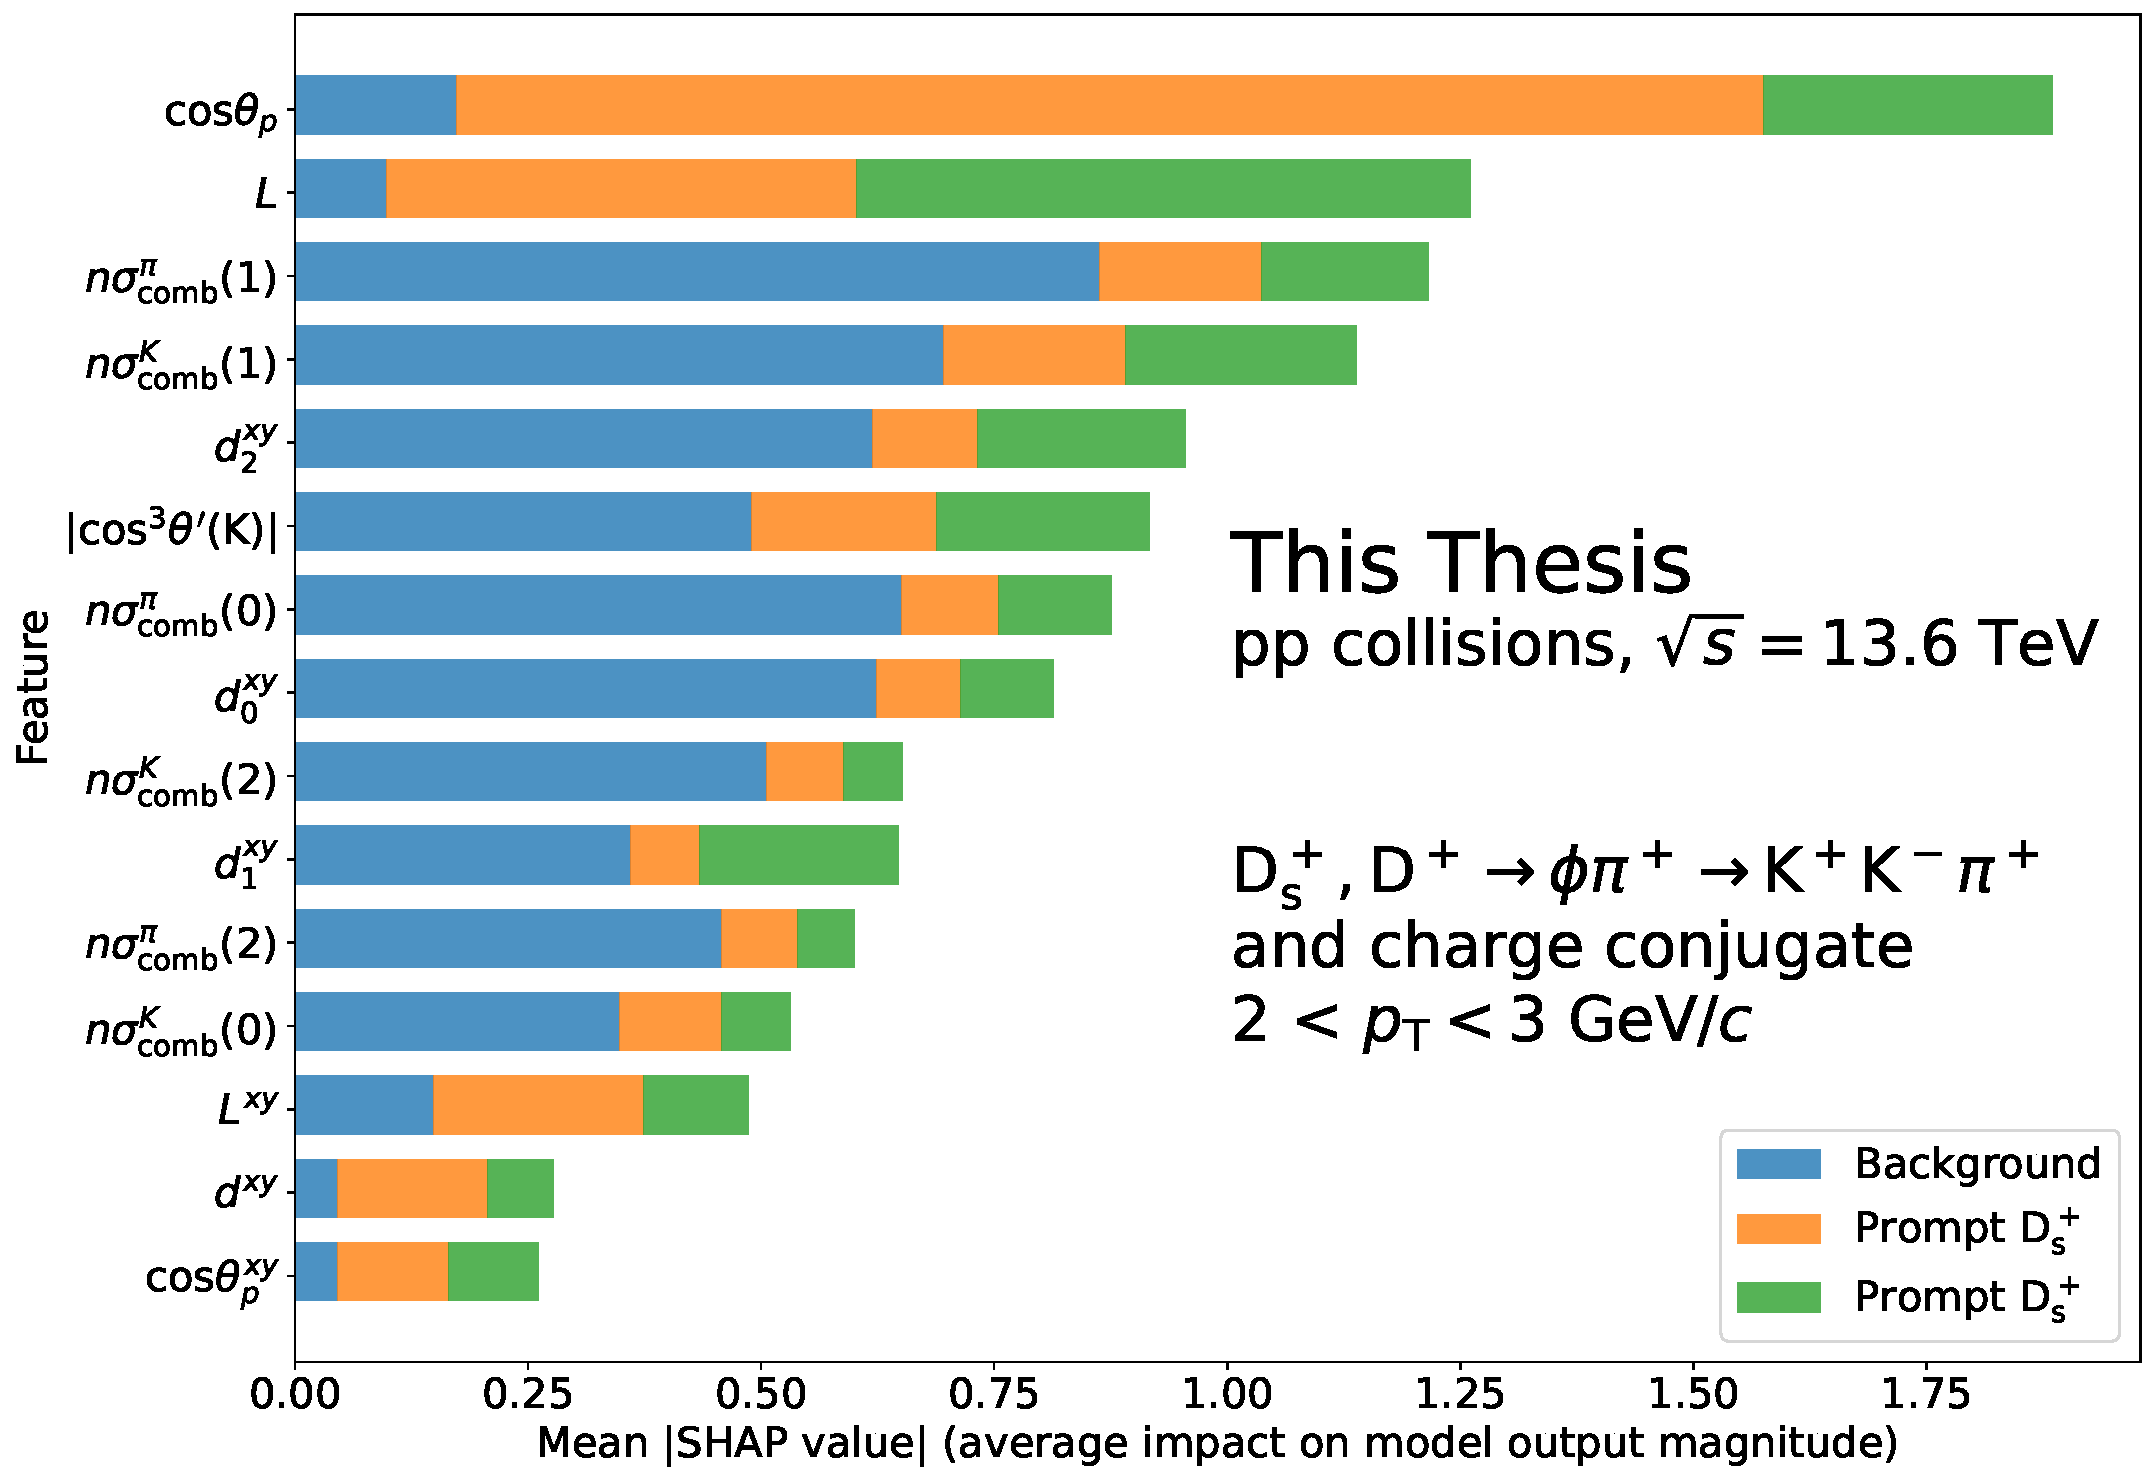
\includegraphics[width=0.48\textwidth]{Figures/Chapter 5/SHAP_summary2_3.pdf}
    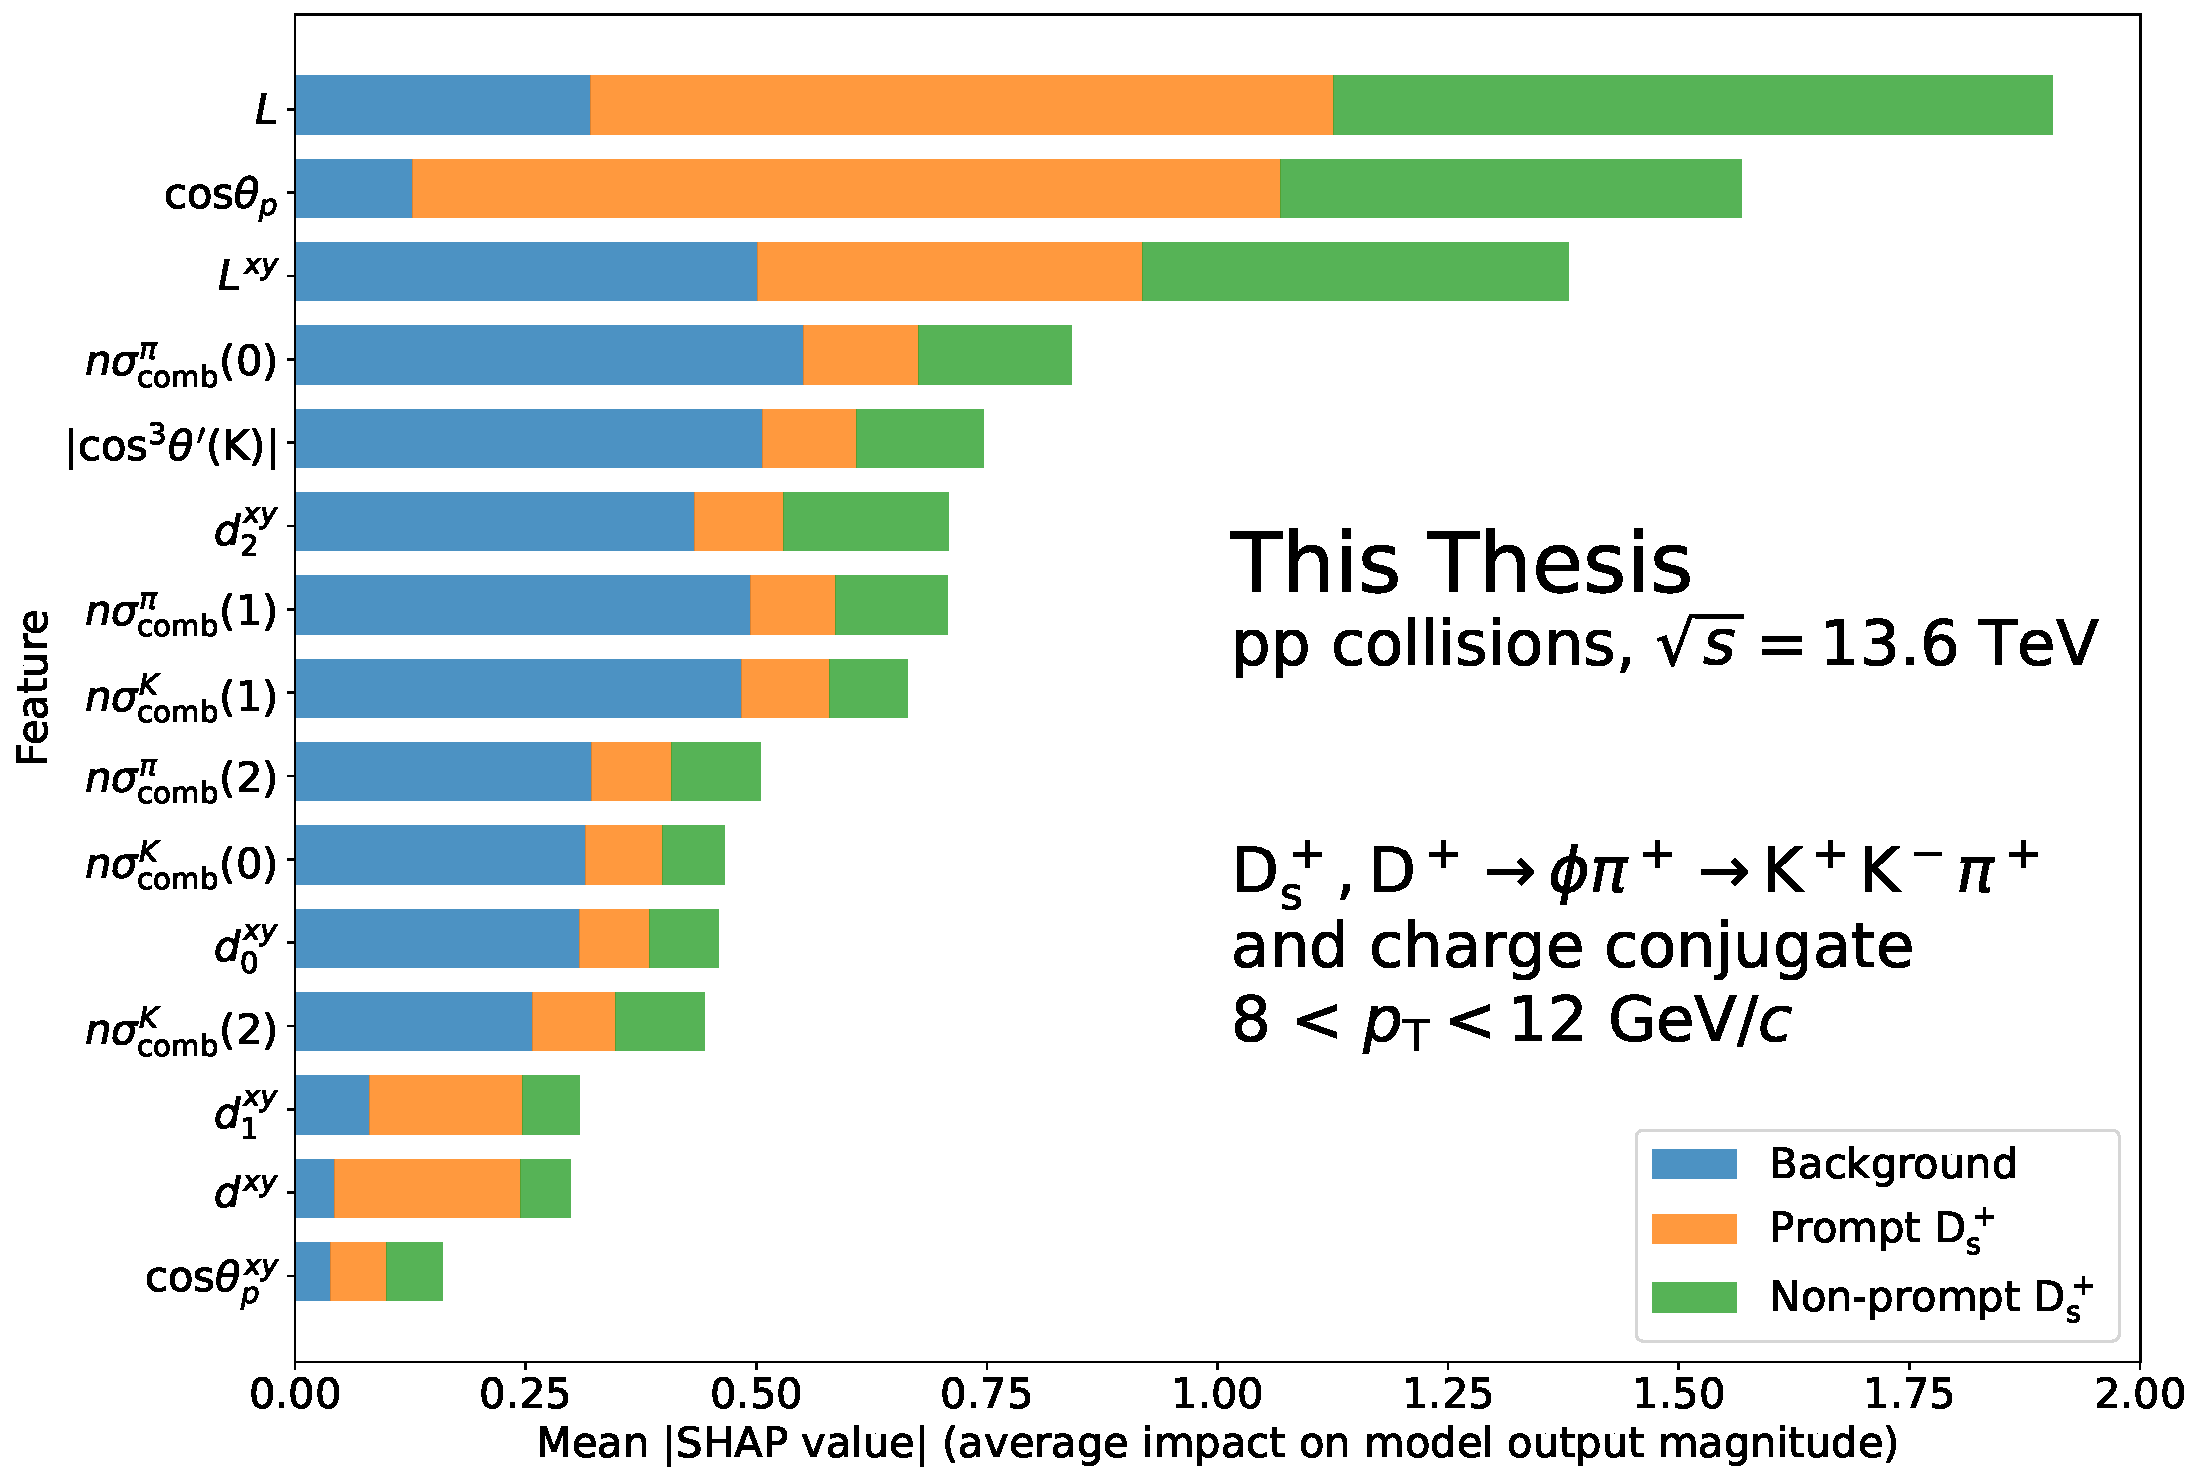
\includegraphics[width=0.48\textwidth]{Figures/Chapter 5/SHAP_summary8_12.pdf}
    \caption{Average $|\text{SHAP value}|$ feature importance for the XGBoost model trained on the \mbox{$2<\pt<3$~\gevc} (left panel) and \mbox{$8<\pt<12$~\gevc} (right panel) intervals. The feature importance for the background, prompt \ds-meson, and non-prompt \ds-meson classes are shown with blue, orange, and green bars, respectively.}
    \label{fig:ml_feature_importance_average}
\end{figure}

\subsection{Optimisation of the selection thresholds on the BDT scores}
Once the model performance has been validated, a set of selection criteria on the BDT output scores has to be chosen to select the candidates. This is a crucial step of the analysis, as it will define the signal selection efficiency and the background contamination. Since the model's output consists of a score related to the probability of belonging to each class, and the three probabilities sum up to unity, the selection criteria have a total of two degrees of freedom. A first selection is applied on the maximum probability to be a background candidate, and rejects most of the contamination from the combinatorial background. The second one is applied on the minimum probability of being a prompt \ds-meson candidate, and suppresses the signal contribution arising from non-prompt \ds-meson candidates. 

A first indication of the optimal selection criteria can be obtained by studying the model's output distributions, e.g., those reported in Fig.~\ref{fig:ml_score}. A good working point can be chosen as the point where a good separation between the three classes is achieved. For this analysis, however, the statistical significance of the extracted inclusive signal (i.e., of both prompt and non-prompt D mesons) is used to define the optimal selection criteria. For each \pt interval of the analysis, the signal $S$ and the background $B$ are evaluated by fitting the invariant mass distribution of candidates from the data passing the different ML selections considered in the optimisation process. Only a subset of the full dataset, corresponding to approximately 3\% of the available data sample is used in this process. The working point is chosen using different considerations. Firstly, the selection criteria are chosen to maximise the statistical significance of the signal, defined as $S/\sqrt{S+B}$. This definition of statistical significance is equivalent to the inverse of the relative statistical uncertainty on the signal, for a Poisson distribution of candidate counts. Thus, maximising the statistical significance corresponds to minimising the relative statistical uncertainty on the signal. In order to avoid an over-optimisation of the model to enhance the statistical significance (which could bias the results if statistical fluctuations are not properly taken into account), the considered threshold values on the BDT output scores are multiples of 0.05. Additionally, the efficiency of the selection is checked to ensure that it is kept at sufficiently high levels, to reduce possible biases in the final results due to possible imperfections in the MC description of the data. A smooth increasing trend with \pt of the efficiency is also ensured to provide consistency in the tightness of the selection criteria across the different \pt intervals. 

Usually, the maximisation of the statistical significance is avoided in the choice of the selection criteria, as it can lead to a bias in the final results. However, in this case, the optimisation is performed on a very small fraction of the data thanks to the large dataset available, and the bias is expected to be negligible. A different approach to select an optimal working point consists in the optimisation of a pseudo-significance, defined as the ratio of the expected signal and the square root of the sum of the expected signal and the expected background. For each considered selection criterion, the selection efficiency is evaluated on MC simulations, and the expected signal is estimated from the D-meson production cross section provided by FONLL~\cite{Cacciari:1998it} theoretical predictions. The expected background is estimated from a fit of the invariant mass distribution of the candidates in the sidebands of the signal region. This approach avoids the introduction of a bias in the final results, as it is blind to the candidates in the signal region. However, it relies on FONLL predictions and MC simulations. To avoid the introduction of biases in the optimisation due to shortcomings of FONLL predictions or MC simulations, the optimisation of the pseudo-significance is not performed in this analysis.

A result of the working point optimisation is presented in Fig.~\ref{fig:ml_significance} for the \mbox{$2.0<\pt<2.5$~\gevc} interval. The statistical significance of the signal is shown as a function of the BDT output score threshold for the probability of being a prompt \ds meson and a background candidate. The chosen set of selection criteria is shown with a green cross.

The optimal selection criteria for each \pt interval considered in the analysis are reported in Table~\ref{tab:working_point}. Because of the large combinatorial background and the small Lorentz boost of the \ds mesons, which results in a small decay length and a less effective selection based on the displaced topology, the selection criteria in the lowest \pt intervals are chosen to be stringent to extract the signal with a large enough signal-to-background ratio. At higher \pt, the selection criteria are loosened, as the larger decay length of the \ds mesons results in a more effective separation between signal and background candidates. In addition, at higher \pt the combinatorial background is reduced, and the selection criteria can be loosened to increase the signal efficiency. The threshold on the prompt \ds-meson probability is kept at around 0.2 for all \pt intervals. This selection allows a significant reduction of the contamination from non-prompt D mesons in the selected sample, while it does not considerably influence the statistical significance of the signal. In the \mbox{$5.5<\pt<6.0$~\gevc} interval, the threshold is increased to 0.25 to guarantee an increasing trend of the efficiency with \pt.

\begin{figure}
    \centering
    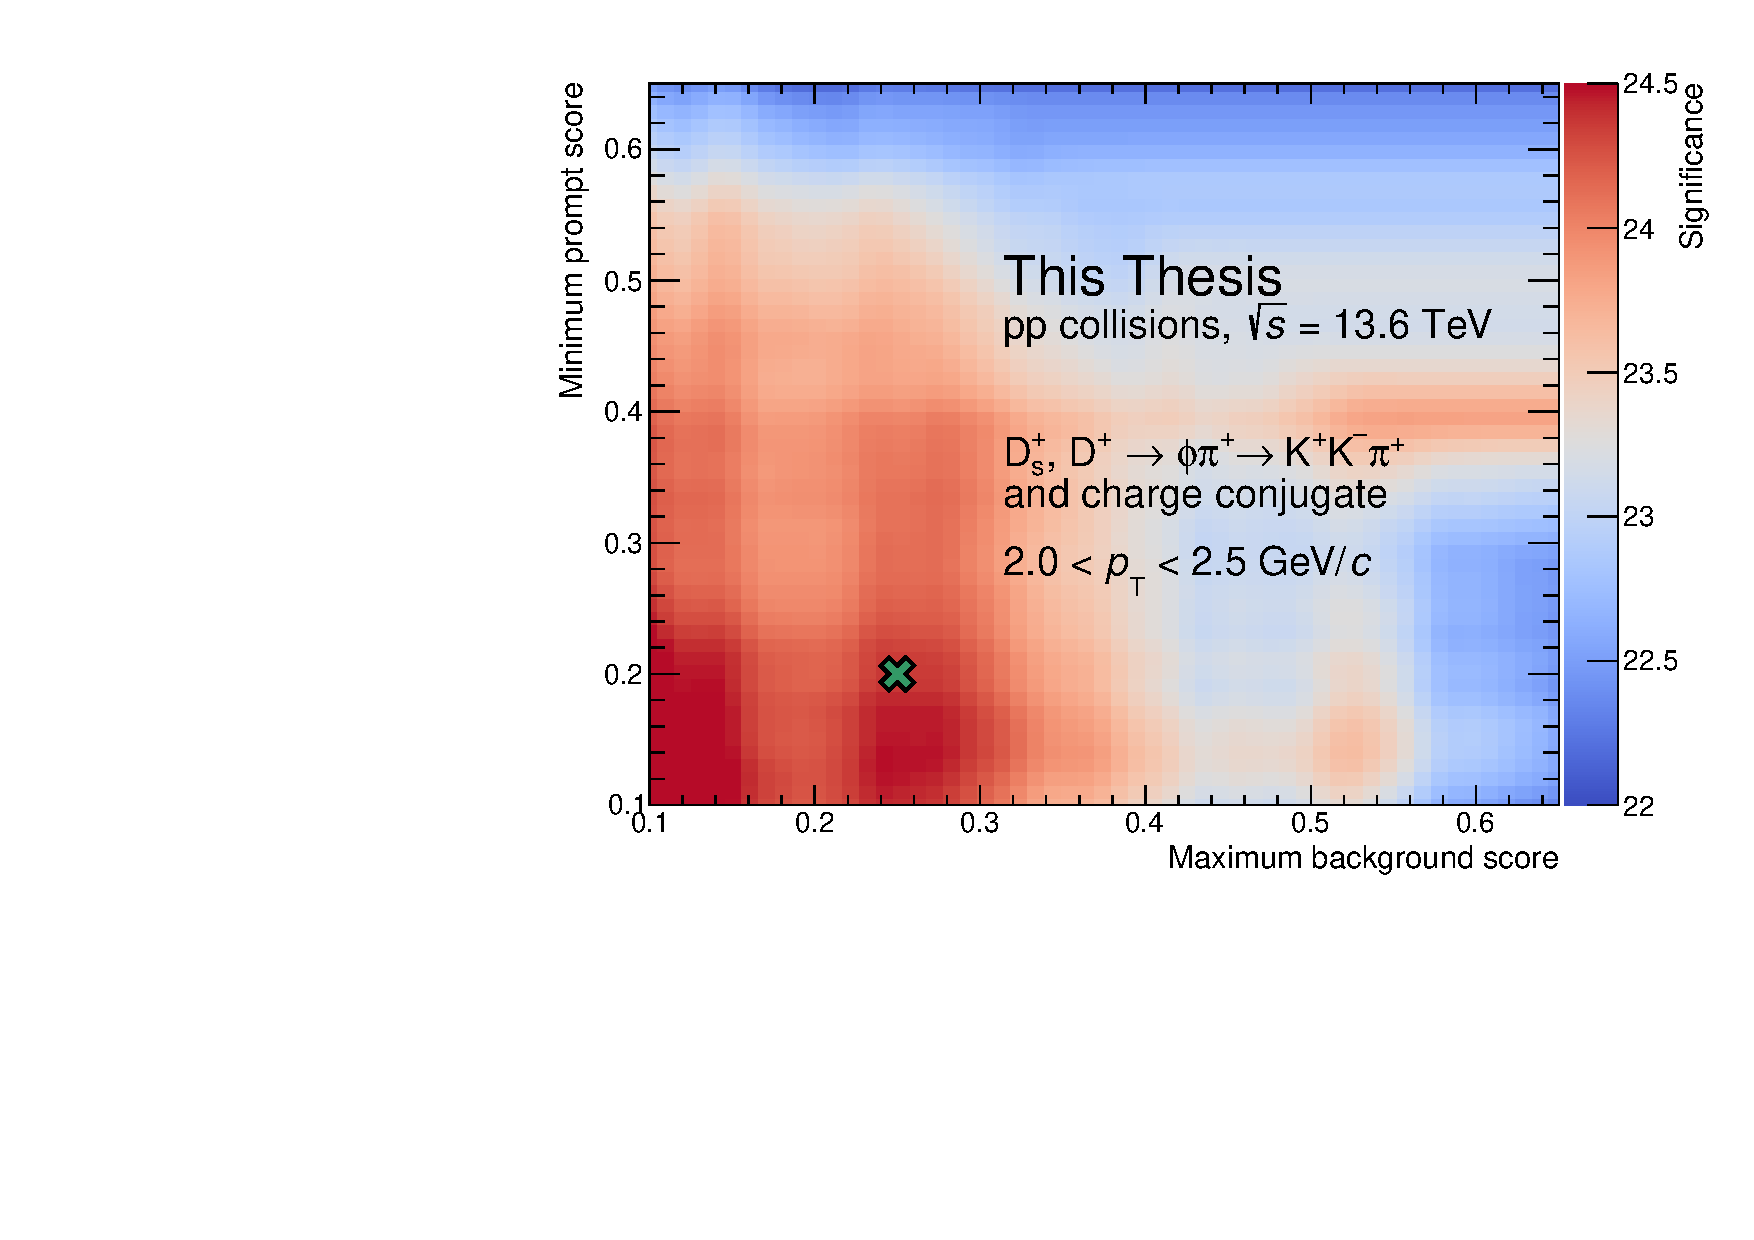
\includegraphics[width=0.7\textwidth]{Figures/Chapter 5/Significance_Scan_2_2p5.pdf}
    \caption{Statistical significance of the signal as a function of the selection criteria applied to the model output for the $2.0<\pt<2.5$~\gevc interval. The chosen set of selection criteria is shown with a green cross.}
    \label{fig:ml_significance}
\end{figure}

\begin{table}[b!]
    \centering
    \caption{Selection criteria applied to enhance the significance of the $\ds$ meson signal in the $\pt$ intervals considered for the analysis.}
    \label{tab:working_point}
    \vspace*{0.3cm}
    \resizebox{\columnwidth}{!}{%
    \begin{tabular}{c|cc}
    \toprule
         \pt interval (\gevc) & Probability to be background $<$ & Probability to be prompt \ds meson $>$  \\
         \midrule
         0.5$-$1.0 & 0.01 & 0.20 \\
         1.0$-$1.5 & 0.05 & 0.20 \\
         1.5$-$2.0 & 0.15 & 0.20 \\
         2.0$-$2.5 & 0.25 & 0.20 \\
         2.5$-$3.0 & 0.30 & 0.20 \\
         3.0$-$3.5 & 0.20 & 0.20 \\
         3.5$-$4.0 & 0.20 & 0.20 \\
         4.0$-$4.5 & 0.20 & 0.20 \\
         4.5$-$5.0 & 0.20 & 0.20 \\
         5.0$-$5.5 & 0.30 & 0.20 \\
         5.5$-$6.0 & 0.30 & 0.25 \\
         6$-$8   & 0.45 & 0.20 \\
         8$-$12  & 0.50 & 0.20 \\
         12$-$24 & 0.55 & 0.20 \\
        \bottomrule
    \end{tabular}%
    }
\end{table}

\section{\texorpdfstring{\ds and \dpl raw-yield extraction}{Ds+ and D+ mesons raw-yield extraction}}

After the working point for the BDT algorithm has been defined, the raw yields of \ds and \dpl mesons are extracted in each \pt interval. They are defined as the sum of particles and antiparticles and are measured in 14 \pt intervals in the range $0.5<\pt<24$~\gevc. The raw yield is extracted by fitting the invariant mass distribution of the selected candidates. 

In several analyses performed by the ALICE Collaboration during the Run~2 data-taking period~\cite{ALICE:2021mgk,ALICE:2023sgl,ALICE:2021kfc}, the raw yield of \ds mesons was extracted by fitting the invariant mass distribution of selected candidates with a probability density function constructed as the sum of a function describing the shape of the combinatorial background (usually an exponential function or a low-order ($<3$) polynomial) and of two Gaussian distributions to model the \ds- and \dpl-meson peaks. The raw yields for the two D-meson species are then obtained by integrating the signal function. 

Figure~\ref{fig:old_fit} shows the fit to the invariant mass distribution of the selected candidates in the \mbox{$1.5<\pt<2.0$~\gevc} interval using the approach described above. Due to the concavity-changing shape of the background, the function chosen to describe the background is a third-order polynomial. This change in the concavity of the background invariant-mass distribution was not observed in previous analyses performed on pp collisions data collected during the LHC Run~2 data-taking period. With the upgrade of the ALICE experimental apparatus, the amount of data collected during the ongoing LHC Run~3 data-taking period is significantly larger than that collected during Run~2, as described in Chapter~\ref{chap:ALICE}. With the increased number of candidates available, the statistical precision of the data sample is higher, and the concavity-changing shape of the background becomes more evident. The small number of candidates available in the Run~2 data sample did not allow for the observation of this feature, as statistical uncertainties covered the shape of the background. On top of the previously-unobserved peculiar shape of the background, the fitting function is not able to describe the data accurately between the two peaks, overestimating the data in this invariant mass region.

\begin{figure}[htb]
    \centering
    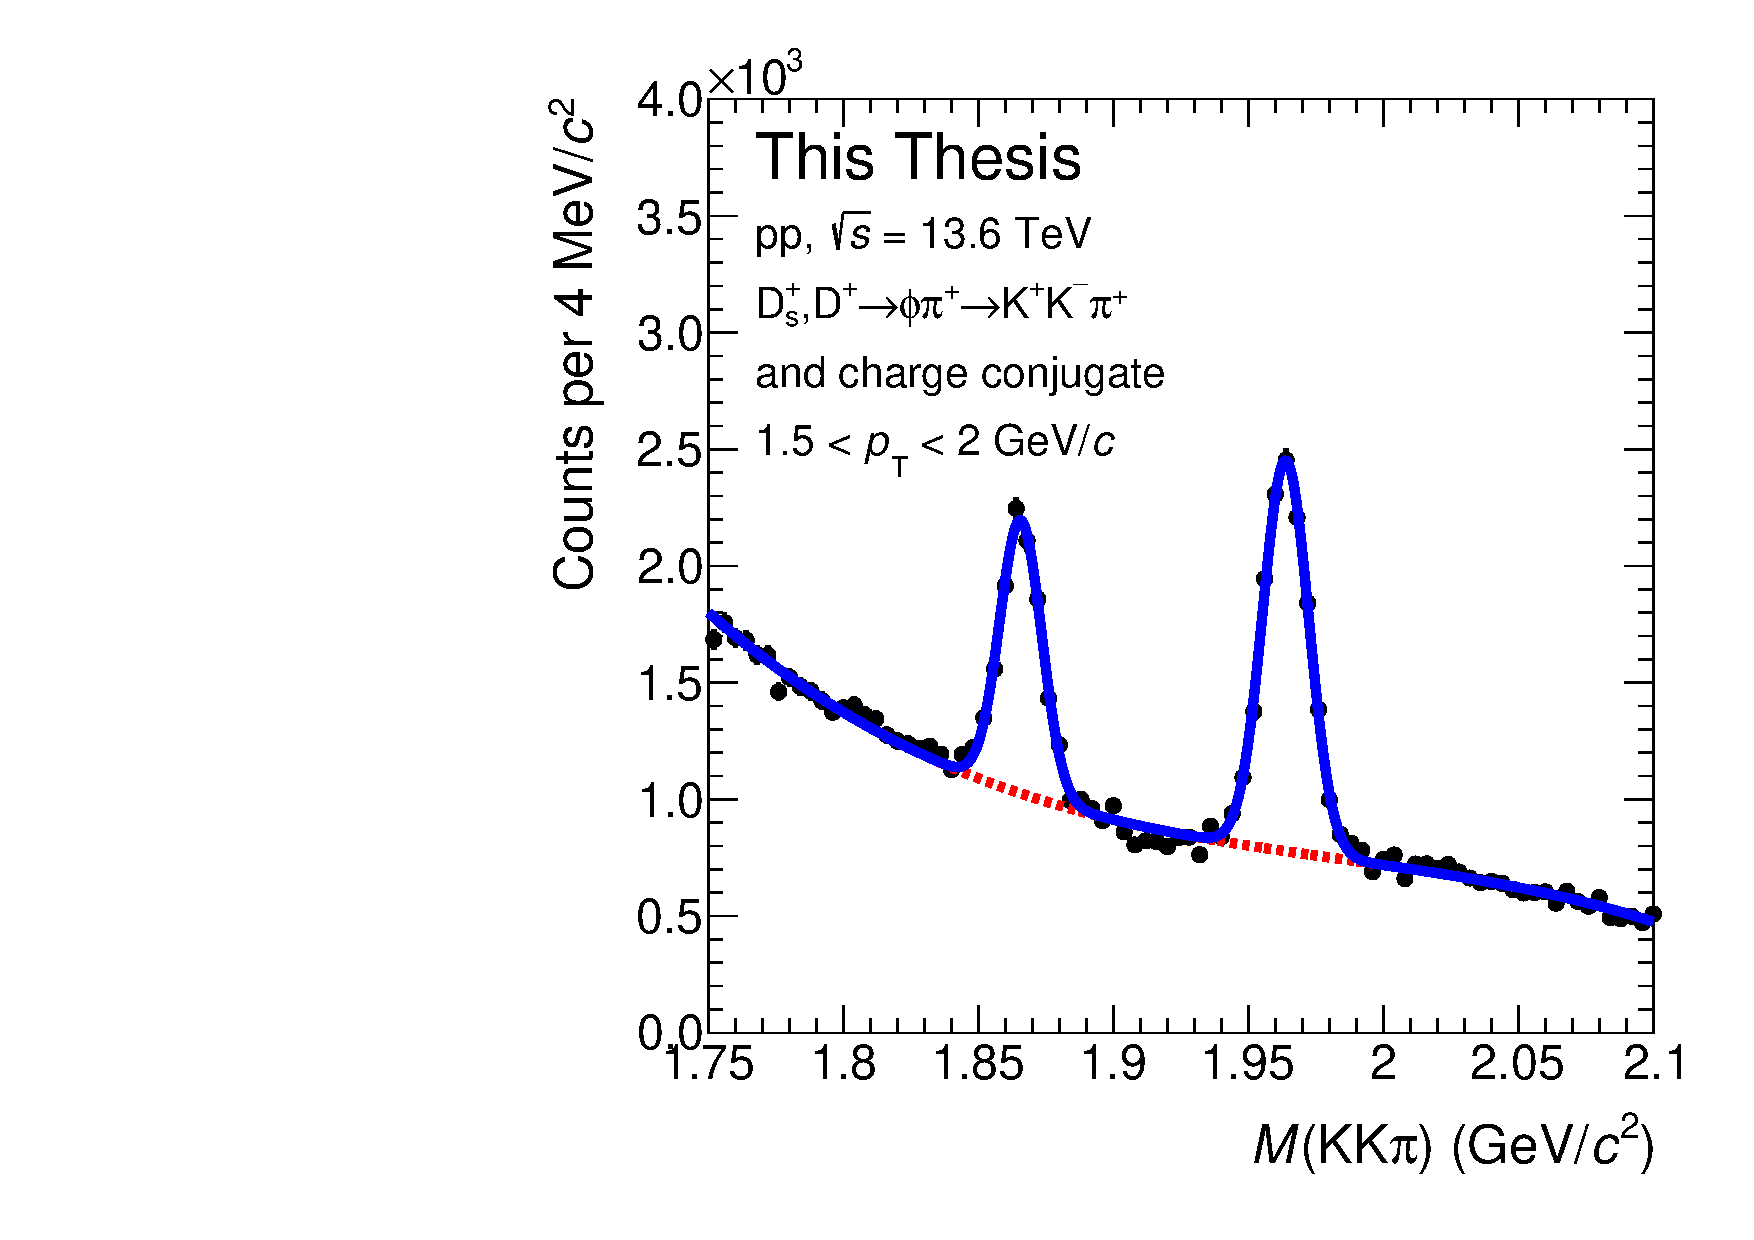
\includegraphics[width=0.7\textwidth]{Figures/Chapter 5/InvMassFitDs1p5_2.pdf}
    \caption{Fit to the invariant mass distribution of selected candidates in the \mbox{$1.5<\pt<2.0$~\gevc} interval. The fit function is shown as a solid line, while the signal and background components are shown as dashed lines. The background is modelled with a third-order polynomial function.}
    \label{fig:old_fit}
\end{figure}

These two features can be understood as due to the fact that the background does not solely arise from the combination of independent tracks, i.e., the combinatorial background. Other physics processes can contribute to the contamination of the data sample, giving rise to a \emph{correlated background}. One such process is the decay of \dpl mesons into the $\dpl\rightarrow\mathrm{\pi^+K^-\pi^+}$ decay channel, where one of the pions is misidentified as a kaon. Despite being suppressed by the applied PID and ML selections, this contribution can give rise to a noticeable contribution due to the large BR of $9.38\%$~\cite{pdg}.

\begin{sloppypar}
To validate this hypothesis, a simulation of \dpl-meson decays into \mbox{$\dpl\rightarrow\mathrm{\pi^+K^-\pi^+}$} was run using \textsc{Pythia}~8~\cite{Bierlich:2022pfr}. Ten billion \dpl mesons were produced with a uniformly distributed \pt spectrum in the $0<\pt<24$~\gevc interval. The \dpl mesons were then forced to decay into the $\dpl\rightarrow\mathrm{\pi^+K^-\pi^+}$ decay channel. For each decay, two invariant masses were evaluated, by assigning the kaon mass to one of the two pions to simulate the misidentification of one pion, while the correct masses were assigned to the other two prongs. The invariant mass distributions obtained from the simulation are shown in Fig.~\ref{fig:DplusSimulations} for different \pt intervals. The distribution is characterised by a peak at $\sim 2$~\gevcc, well inside the fit range used to extract the raw yield of \ds and \dpl mesons in Fig~\ref{fig:old_fit}. In addition, the invariant mass distribution evolves with the \pt of the \dpl meson, with a tail towards higher invariant masses for higher \pt values. This follows naturally from the kinematic properties of the decay. Other sources of correlated background can be present (e.g., from \lc decays), but their contribution was found to be negligible.
\end{sloppypar}

\begin{figure}[htbp]
    \centering
    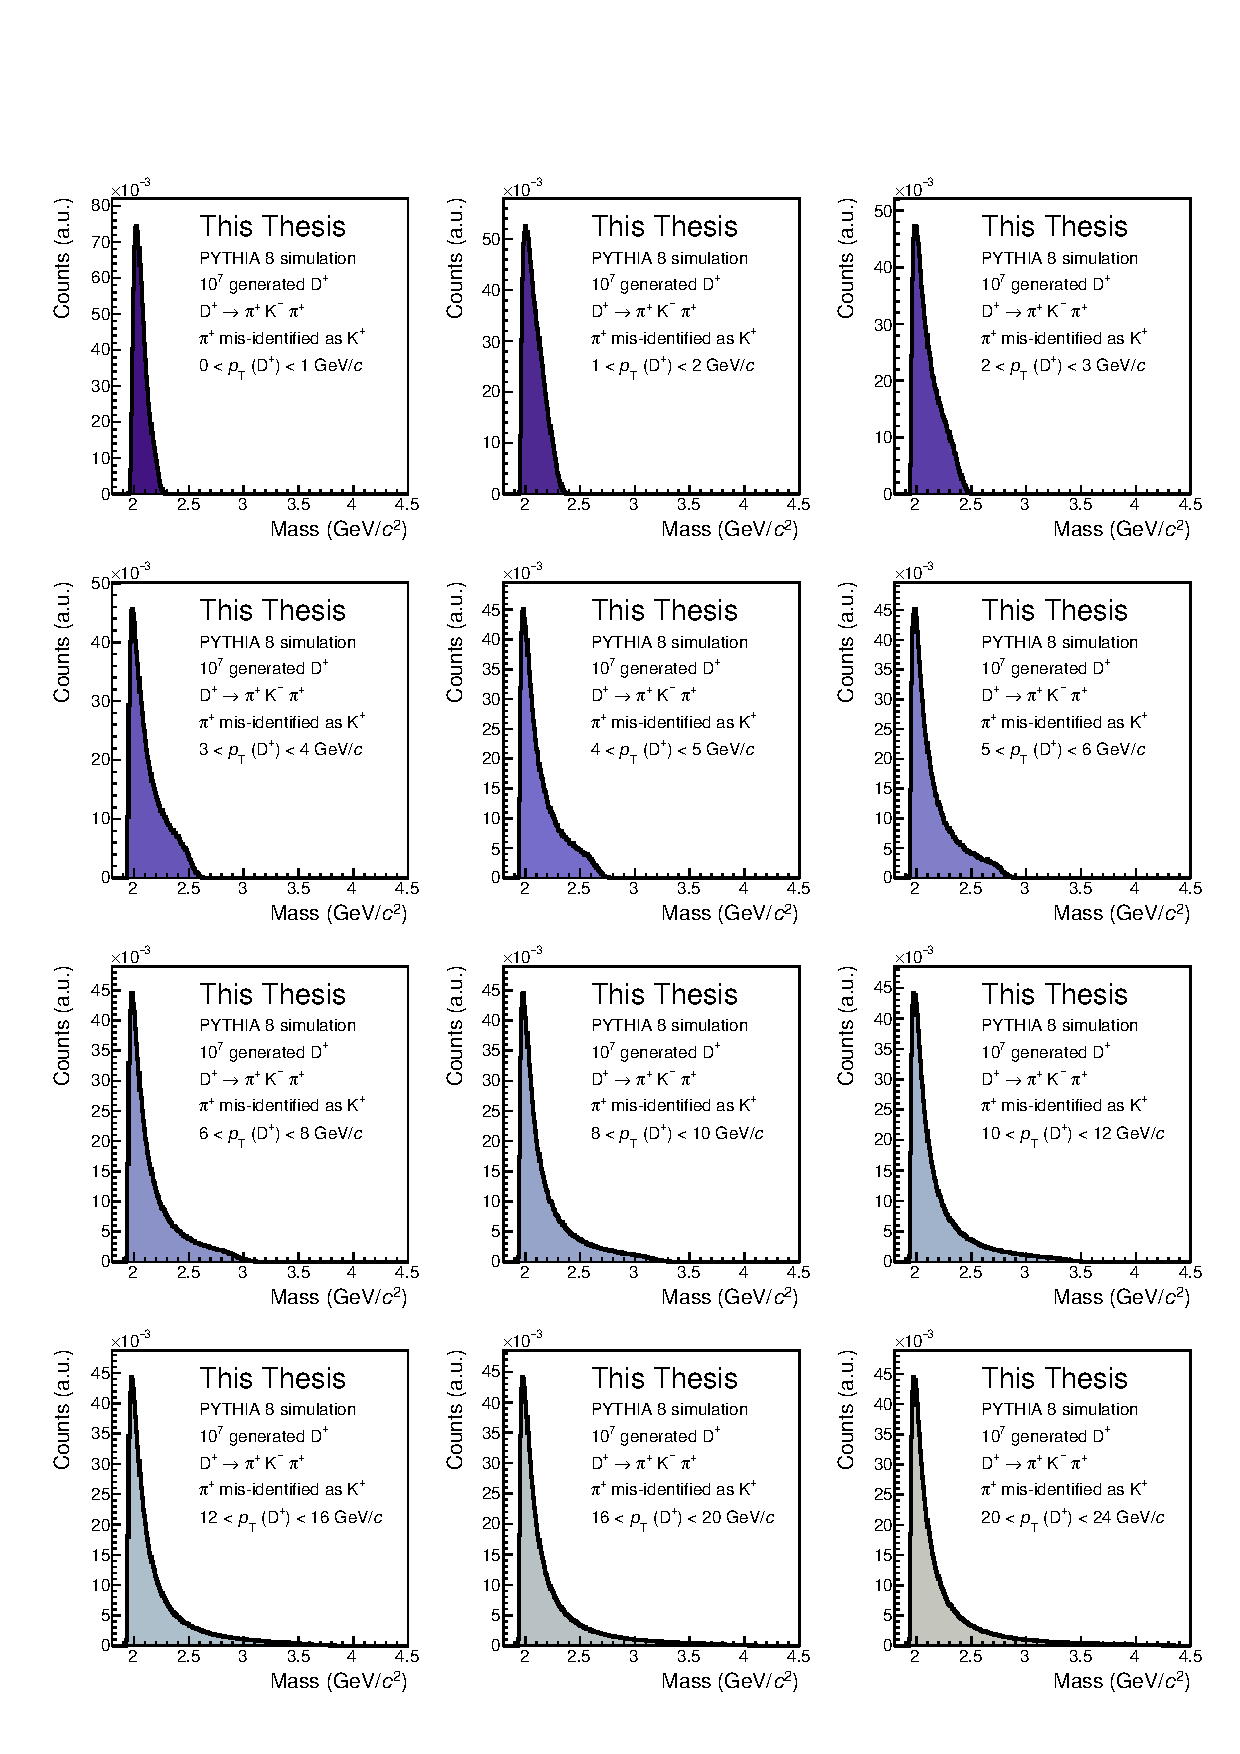
\includegraphics[width=\textwidth]{Figures/Chapter 5/Dplus_Corr_Bkg_simulation.pdf}
    \caption{Invariant-mass distribution of simulated decays of \dpl mesons into \mbox{$\dpl\rightarrow\mathrm{\pi^+K^-\pi^+}$}, where one of the pions produced in the decay is misidentified as a kaon. Distributions for different \pt intervals are shown. }
    \label{fig:DplusSimulations}
\end{figure}

To account for this contribution, a template contribution is included in the fit function, in addition to the combinatorial background and the two signal peaks. This method involves fitting the invariant mass distribution using a predefined template to model the misidentified $\dpl\rightarrow\mathrm{\pi^+K^-\pi^+}$ decay, whose shape is fixed, and the only adjustable parameter is the normalisation. The shape of the template is taken from the same simulation used to train the BDT model, as described in Sec.~\ref{sec:ml_data_preparation}, where $\dpl\rightarrow\mathrm{\pi^+K^-\pi^+}$ mesons reconstructed as $\dpl\rightarrow\mathrm{K^+K^-\pi^+}$, passing PID selections as $\mathrm{K^+K^-\pi^+}$, are selected. The distribution is fixed to that obtained before applying any ML model, as it was studied that the applied ML selections do not affect the shape of the correlated background. This allows for reducing statistical fluctuations in the template shape. The final fit function is then constructed as the sum of a parabolic function to describe the combinatorial background, the template function described above for the correlated $\dpl\rightarrow\mathrm{\pi^+K^-\pi^+}$ background source, and two Gaussian functions to describe the \ds- and \dpl-meson peaks. The signal parameters (mean, width, normalisation), as well as the parameters of the combinatorial background and the normalisation of the template fit are left free in the fit in the \pt intervals below 8~\gevc. Because of the observed momentum resolution worsening at higher \pt, and because of the smaller number of candidates available in the high-\pt intervals, for the $\pt>8$~\gevc range the widths of the \dpl-meson signal peaks are fixed to those of the \ds meson divided by a factor 1.2, which is the observed ratio of the peak widths at low \pt, with a flat trend with \pt, as illustrated in Fig.~\ref{fig:sigma_ratio}. In the left panel, the evolution of the peak widths of the \ds and \dpl mesons as a function of \pt is shown for both data and MC simulations. A clear increasing trend of the peak widths with \pt is observed because of the degrading momentum resolution due to the decreasing track curvature. MC simulations underestimate the peak widths extracted from the data for both \ds and \dpl mesons, across the studied \pt range. In the right panel of Fig.~\ref{fig:sigma_ratio}, the ratio between the peak widths of the \ds and \dpl mesons is shown as a function of \pt, for both data and MC simulations. The ratio is observed to be almost constant across the analysed \pt range, with a value of $\sim 1.2$. The ratio is underestimated by the MC simulations, which predict a value of $\sim 1.1$ across the studied \pt range.

In the \pt interval above 8~\gevc, where the peak width of the \dpl meson is fixed to that of the \ds meson divided by a factor of 1.2, a first fit is performed by keeping both peak widths as free parameters. Then, the \dpl-meson peak width is fixed to that of the \ds divided by 1.2, and the fit is repeated, keeping the remaining parameters free. Additionally, in order to correctly describe the background shape, the fit is performed in the invariant mass range \mbox{$1.73<M(\mathrm{KK\pi})<2.15$~\gevcc} for \mbox{$\pt>5$~\gevc}, while a narrower invariant mass window, \mbox{$1.75<M(\mathrm{KK\pi})<2.1$~\gevcc}, is used at lower \pt. The invariant-mass bin width has been fixed to 2~\mevcc. The fits to the invariant mass distributions of selected D-meson candidates are performed using the \code{flarefly} package~\cite{grosa_2023_7579657}, which provides a flexible Python interface for performing fits. 

\begin{figure}[htb]
    \centering
    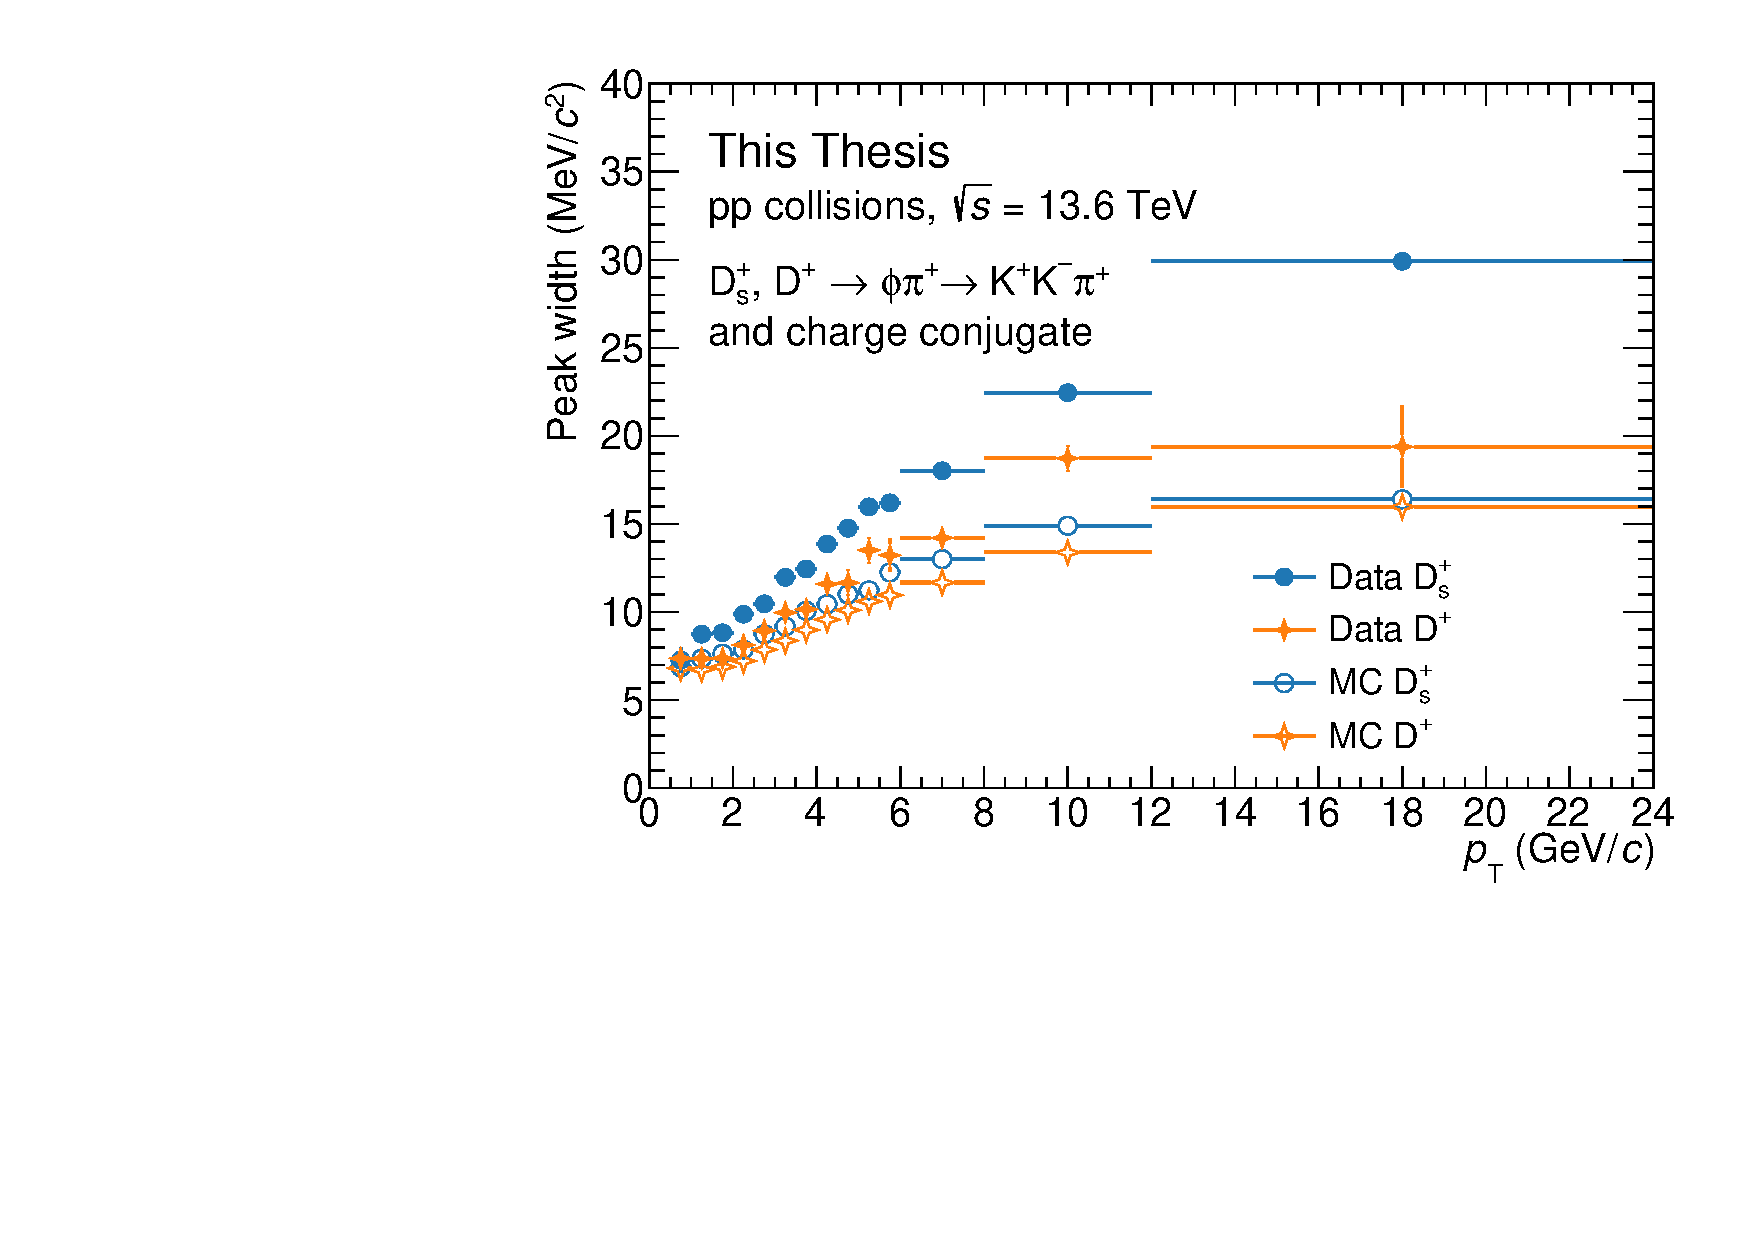
\includegraphics[width=0.48\textwidth]{Figures/Chapter 5/SigmaDs_Dplus.pdf}
    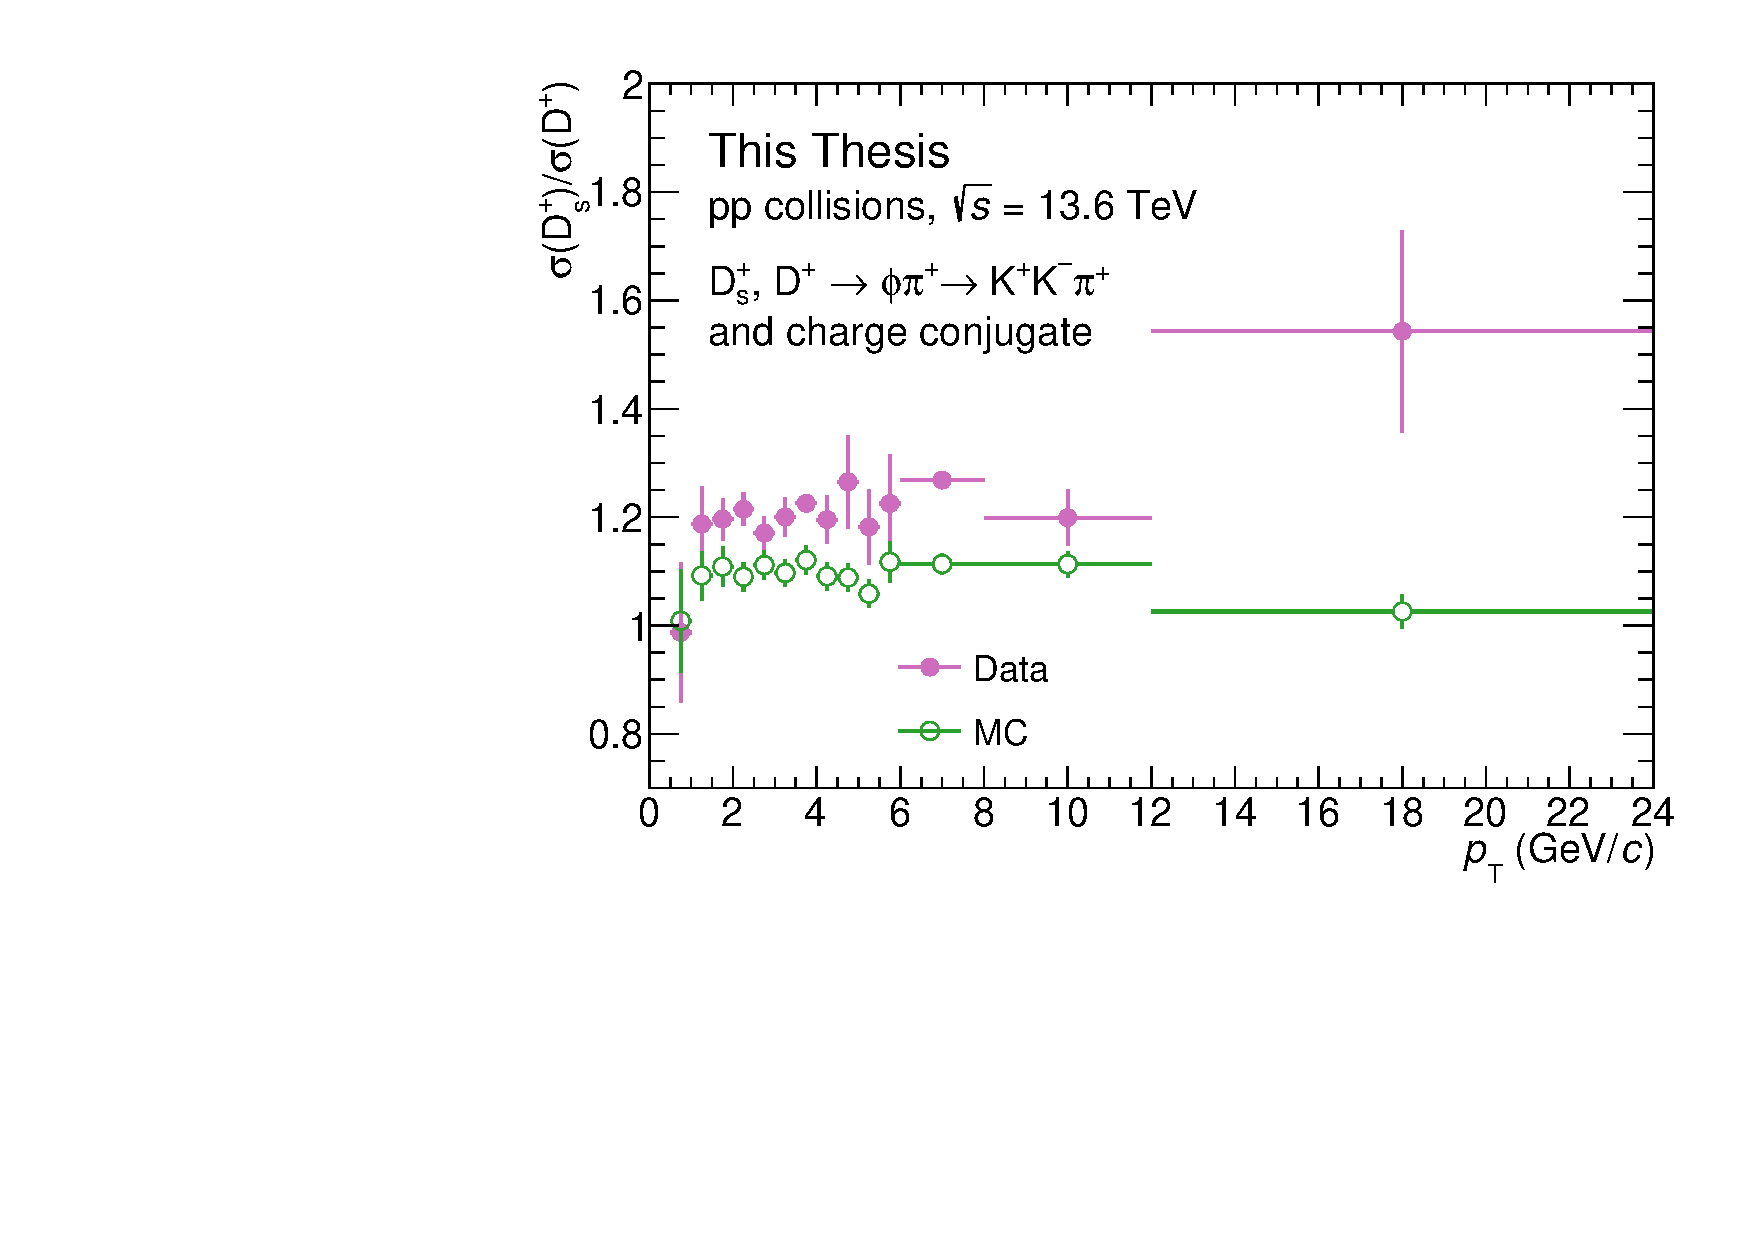
\includegraphics[width=0.48\textwidth]{Figures/Chapter 5/SigmaDsOverDplusMC.pdf}
    \caption{Left panel: peak width of the \ds and \dpl mesons as a function of \pt, before fixing the width of the \dpl meson to that of the \ds meson divided by a factor of 1.2 for $\pt>8~\gevc$. Both the peak widths from fits to data and MC simulations are reported. Right panel: ratio of the peak widths of the \ds and \dpl mesons as a function of \pt, for both data and MC simulations.}
    \label{fig:sigma_ratio}
\end{figure}


The fit to the invariant mass distribution of candidates passing the ML selections is shown in Fig.~\ref{fig:new_fit} for one representative \pt interval of $2.0<\pt<2.5$~\gevc. The total fit function is shown as a solid blue line, the signal contributions are shown as filled green and azure areas for \dpl and \ds mesons, respectively, the combinatorial background is represented with a solid red line, while the correlated background is shown as a dashed violet line. The fit is able to describe the data accurately, as can be deduced from the distribution of the difference between the data and the background fit function, shown in the bottom panels for the two \pt bins. 

\begin{figure}[htb]
    \centering
    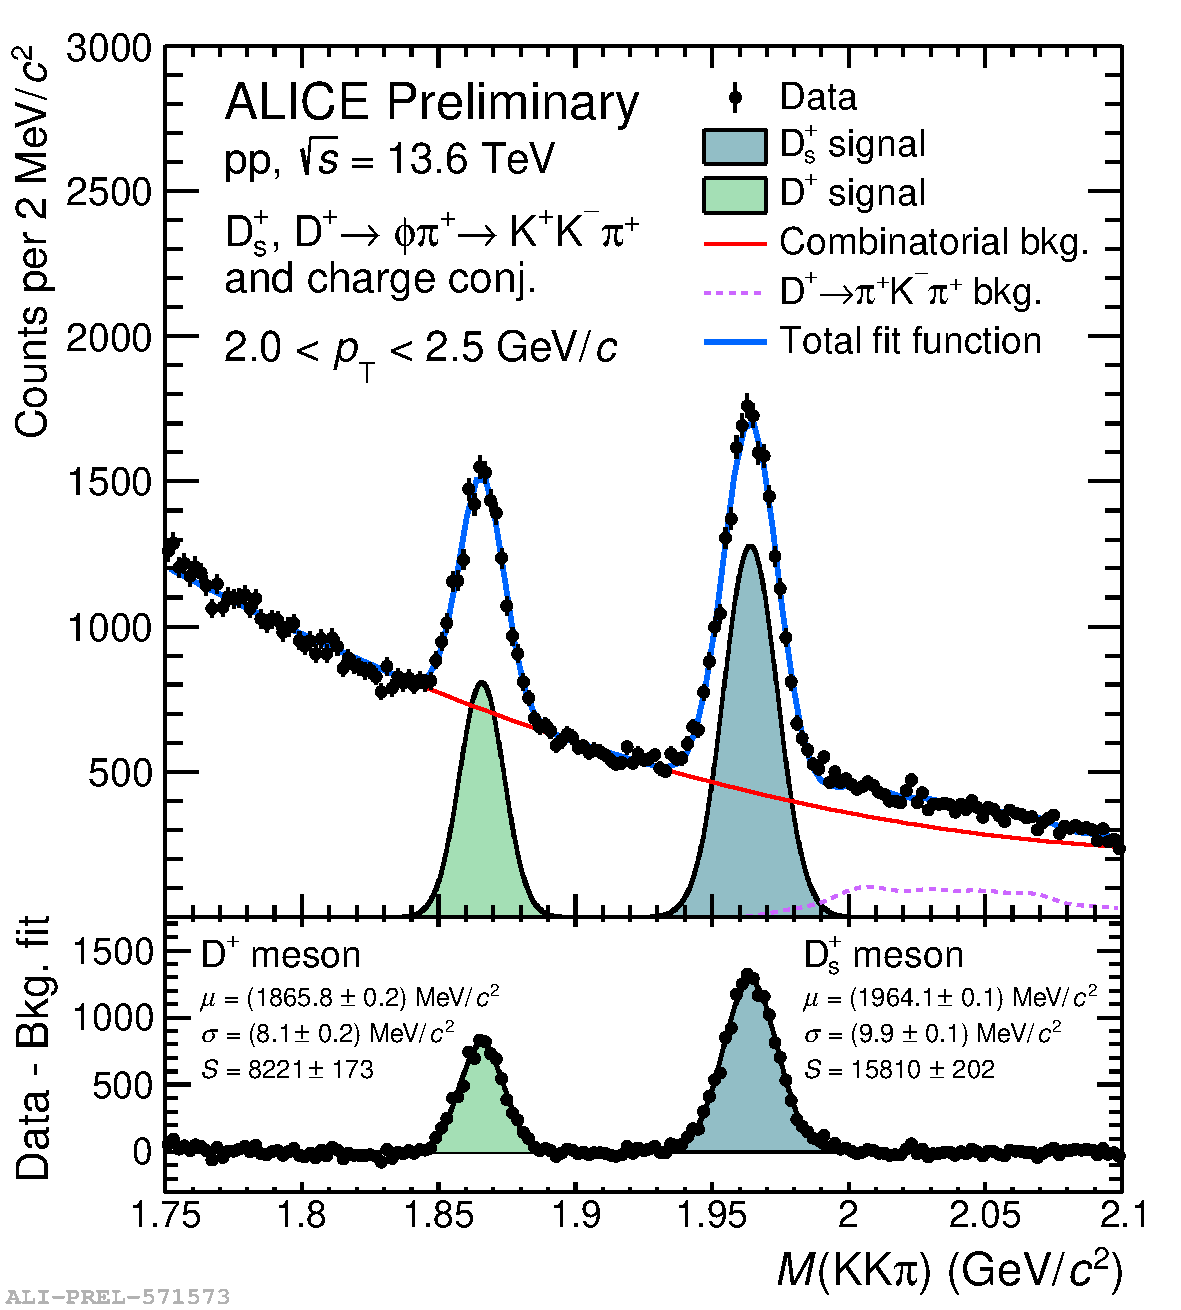
\includegraphics[width=0.7\textwidth]{Figures/Chapter 5/invmassfit_2_2p5.pdf}
    \caption{Fit to the invariant mass distribution of selected candidate in the \mbox{$2.0<\pt<2.5$~\gevc} interval. The total fit function is shown as a solid blue line, while background components are shown as solid red lines (correlated background) and dashed violet lines (dashed violet lines). The signal contributions are shown as filled green and azure areas for \dpl and \ds mesons, respectively. The bottom panels show the distribution of the difference between the data and the background fit function.}
    \label{fig:new_fit}
\end{figure}

The complete set of fits to the invariant mass distributions in the 14 studied \pt intervals is shown in Fig.~\ref{fig:new_fit_all}. All the fits present a good level of agreement between the data and the fit function. Figure~\ref{fig:new_fit_all} also shows that the contribution of the correlated $\dpl\rightarrow\mathrm{\pi^+K^-\pi^+}$ background evolves with \pt, with a larger contribution at lower \pt values. The raw yield of \ds and \dpl mesons is then extracted by integrating the signal function.

\begin{sidewaysfigure}[p]
    \centering
    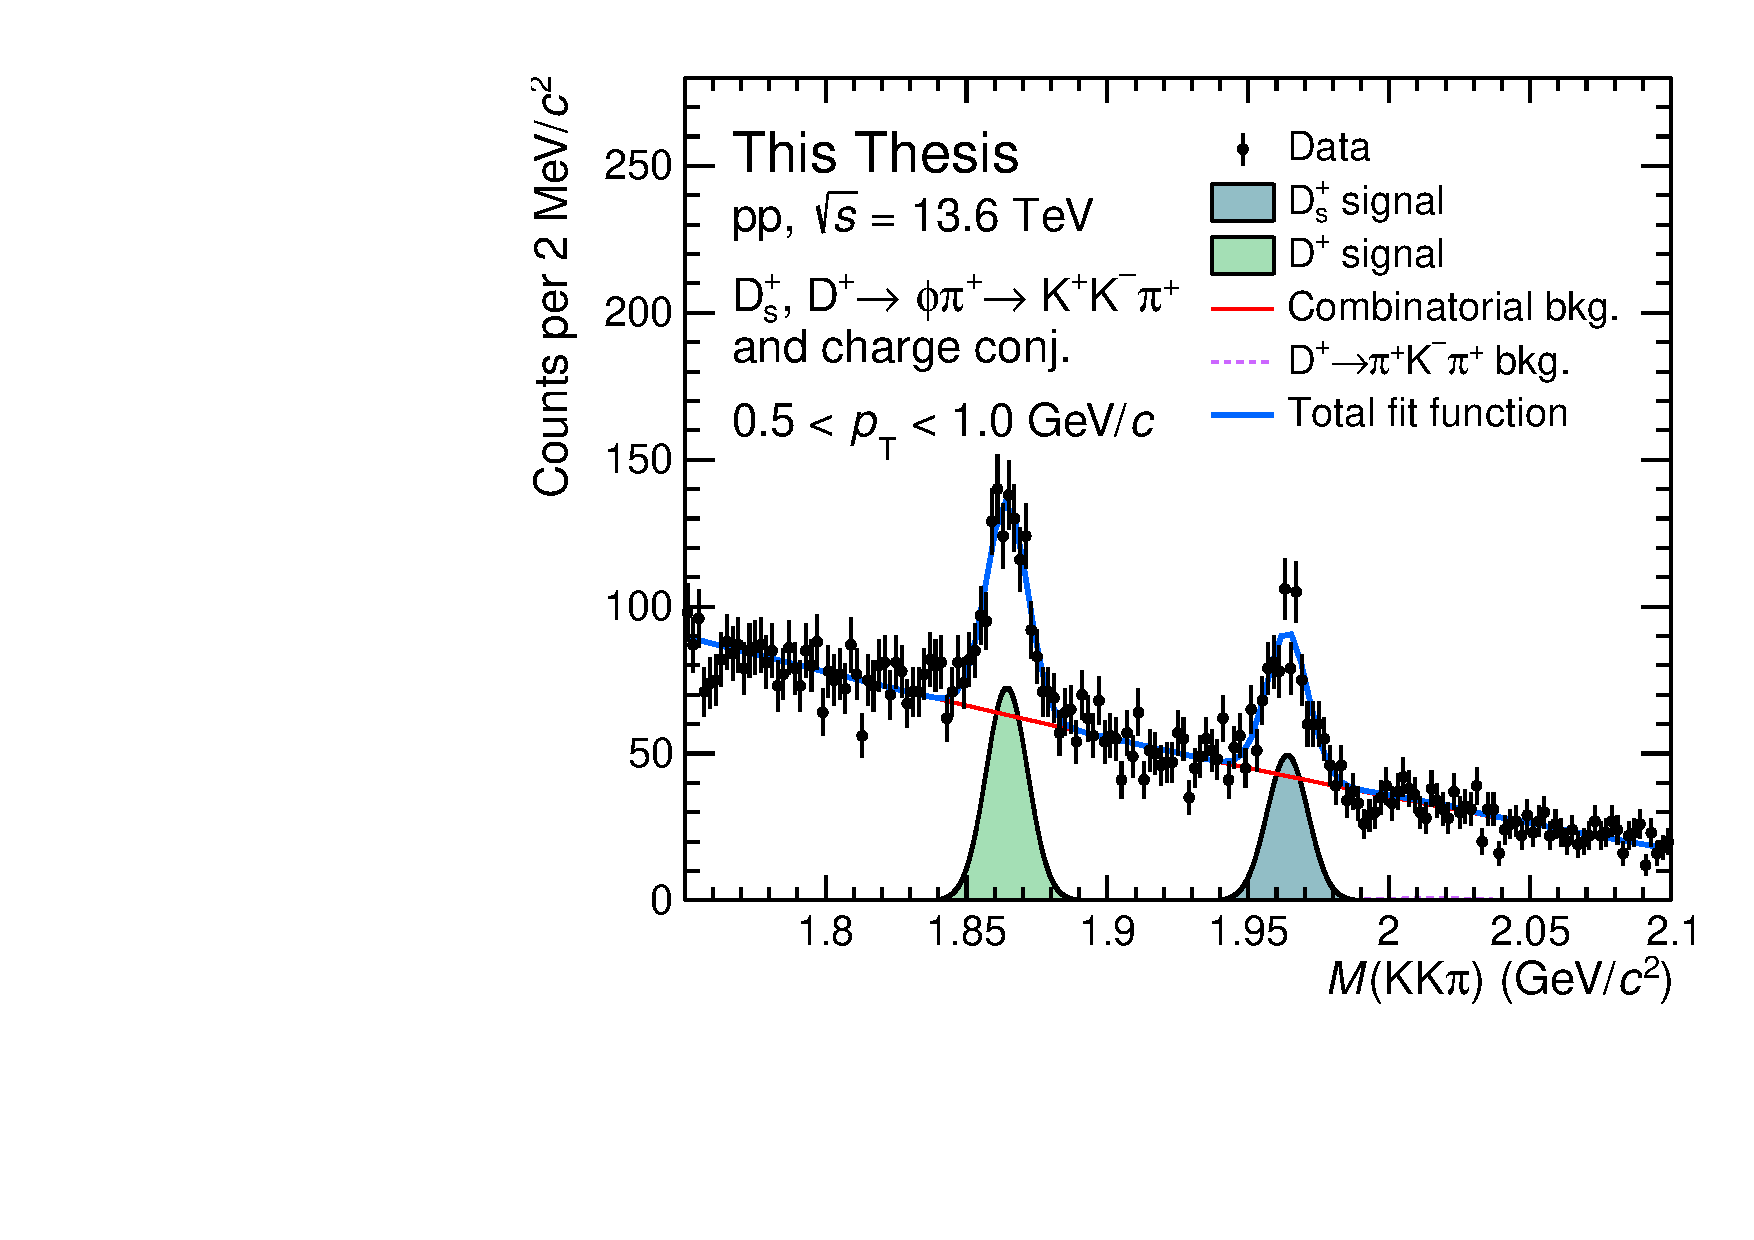
\includegraphics[width=0.2\textwidth]{Figures/Chapter 5/inv_mass/pt_0.5_1.0.pdf}
    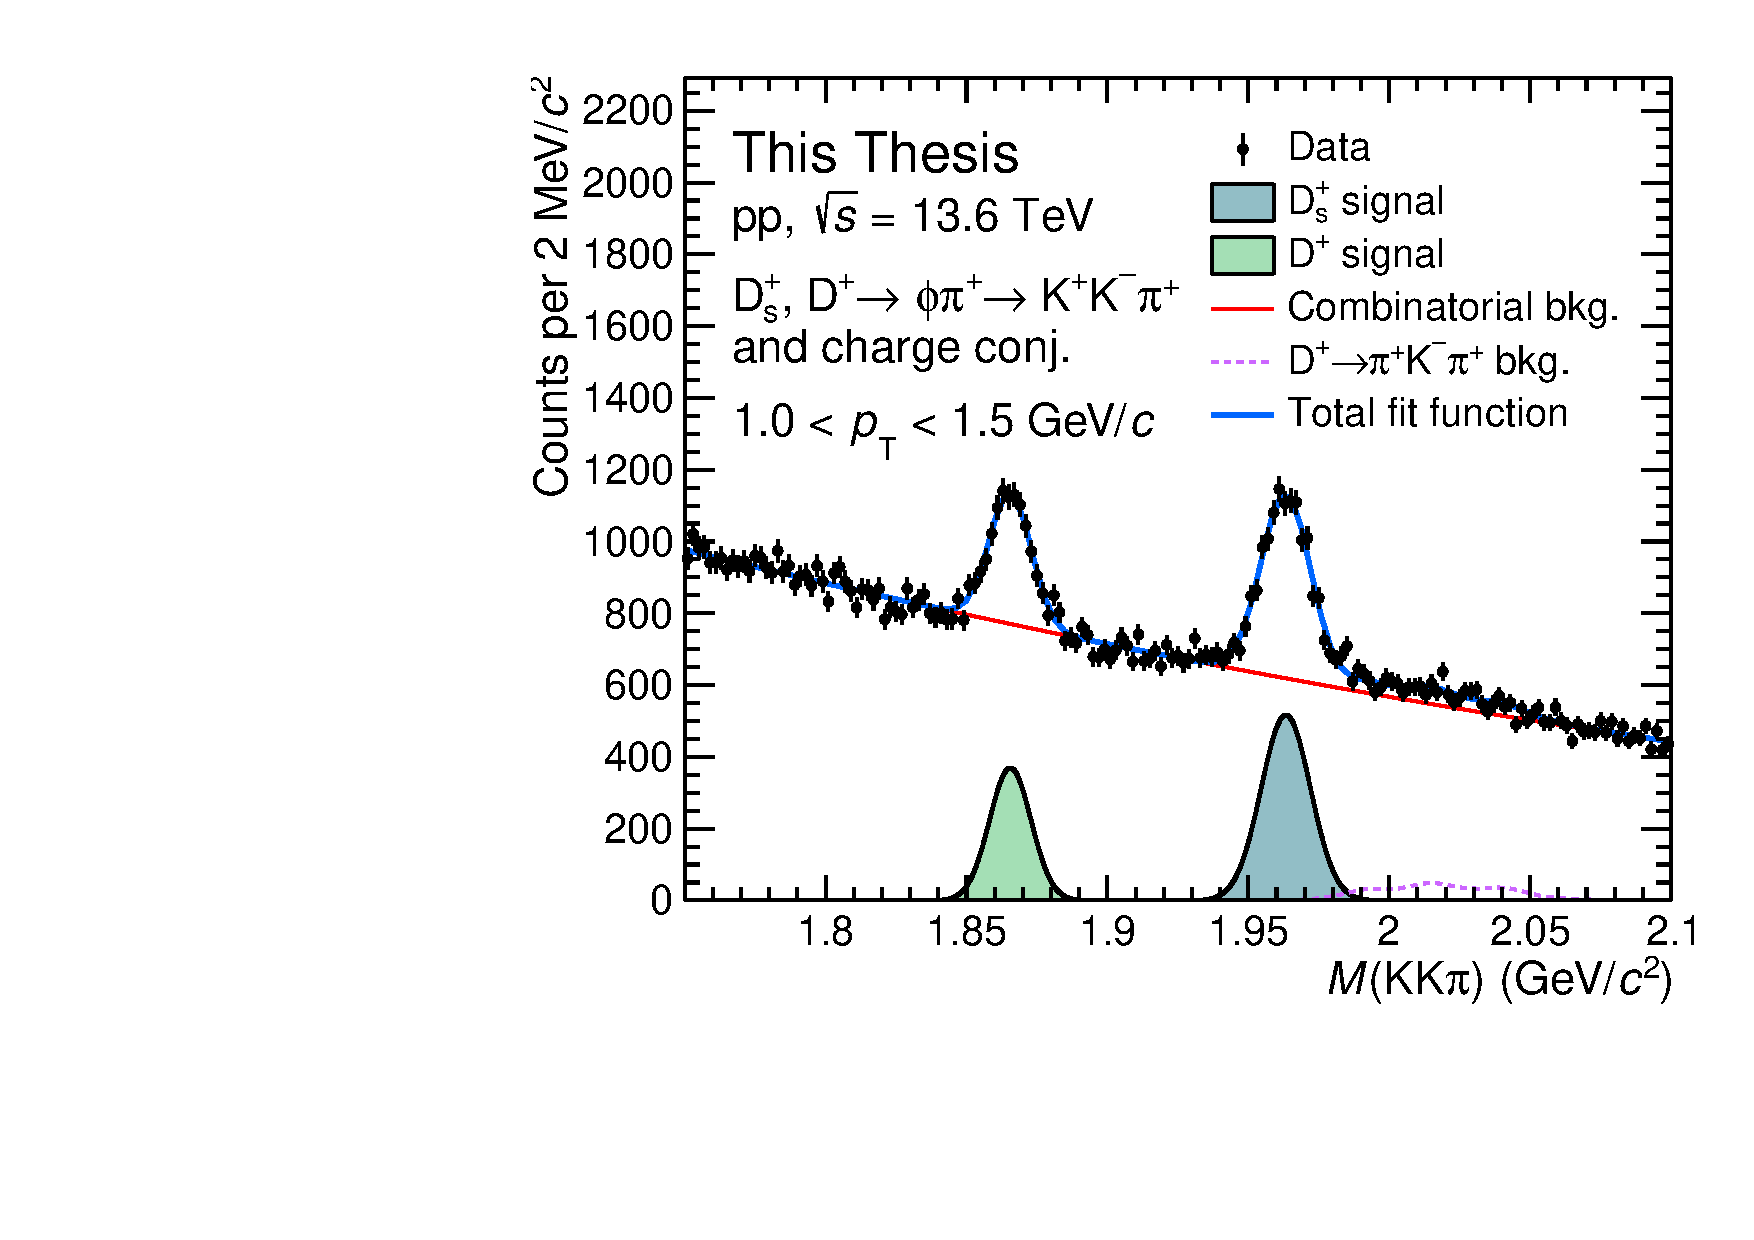
\includegraphics[width=0.2\textwidth]{Figures/Chapter 5/inv_mass/pt_1.0_1.5.pdf}
    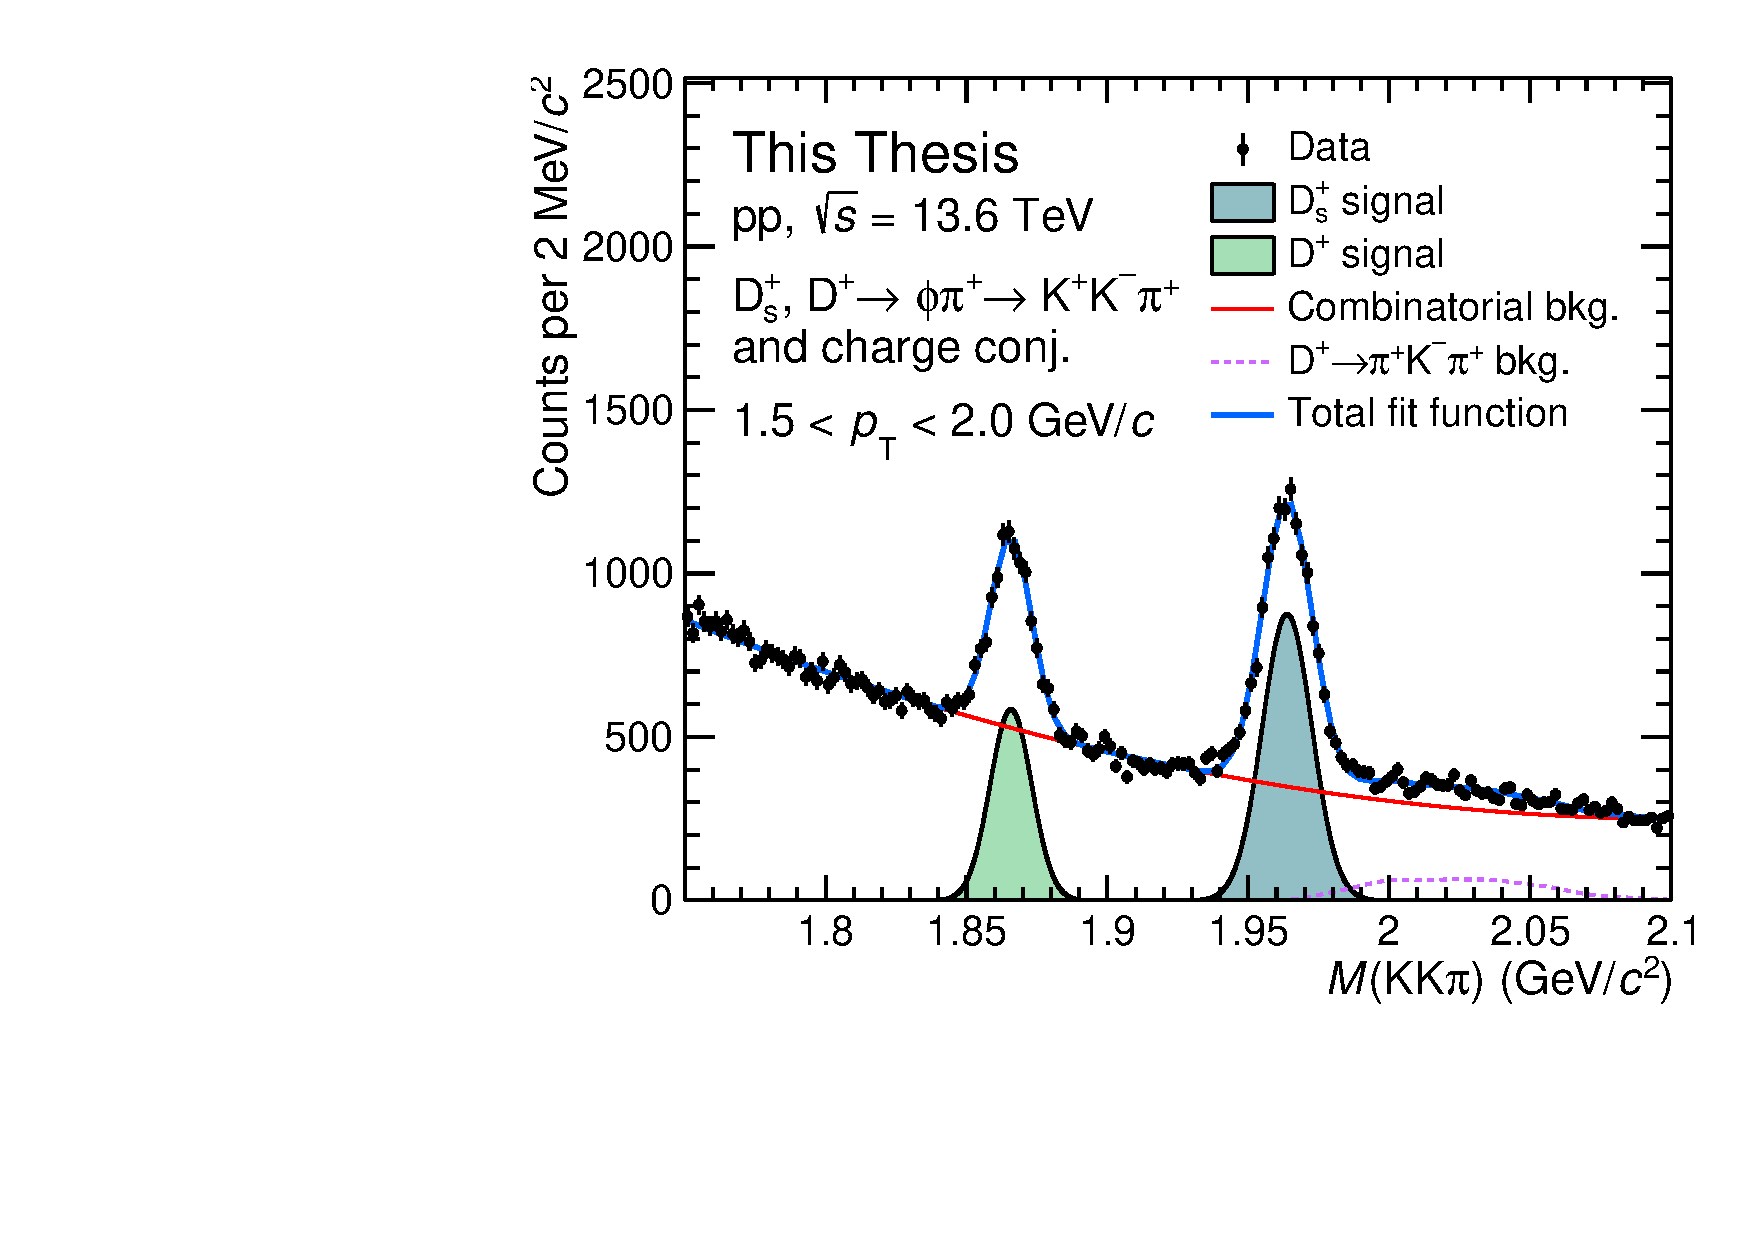
\includegraphics[width=0.2\textwidth]{Figures/Chapter 5/inv_mass/pt_1.5_2.0.pdf}
    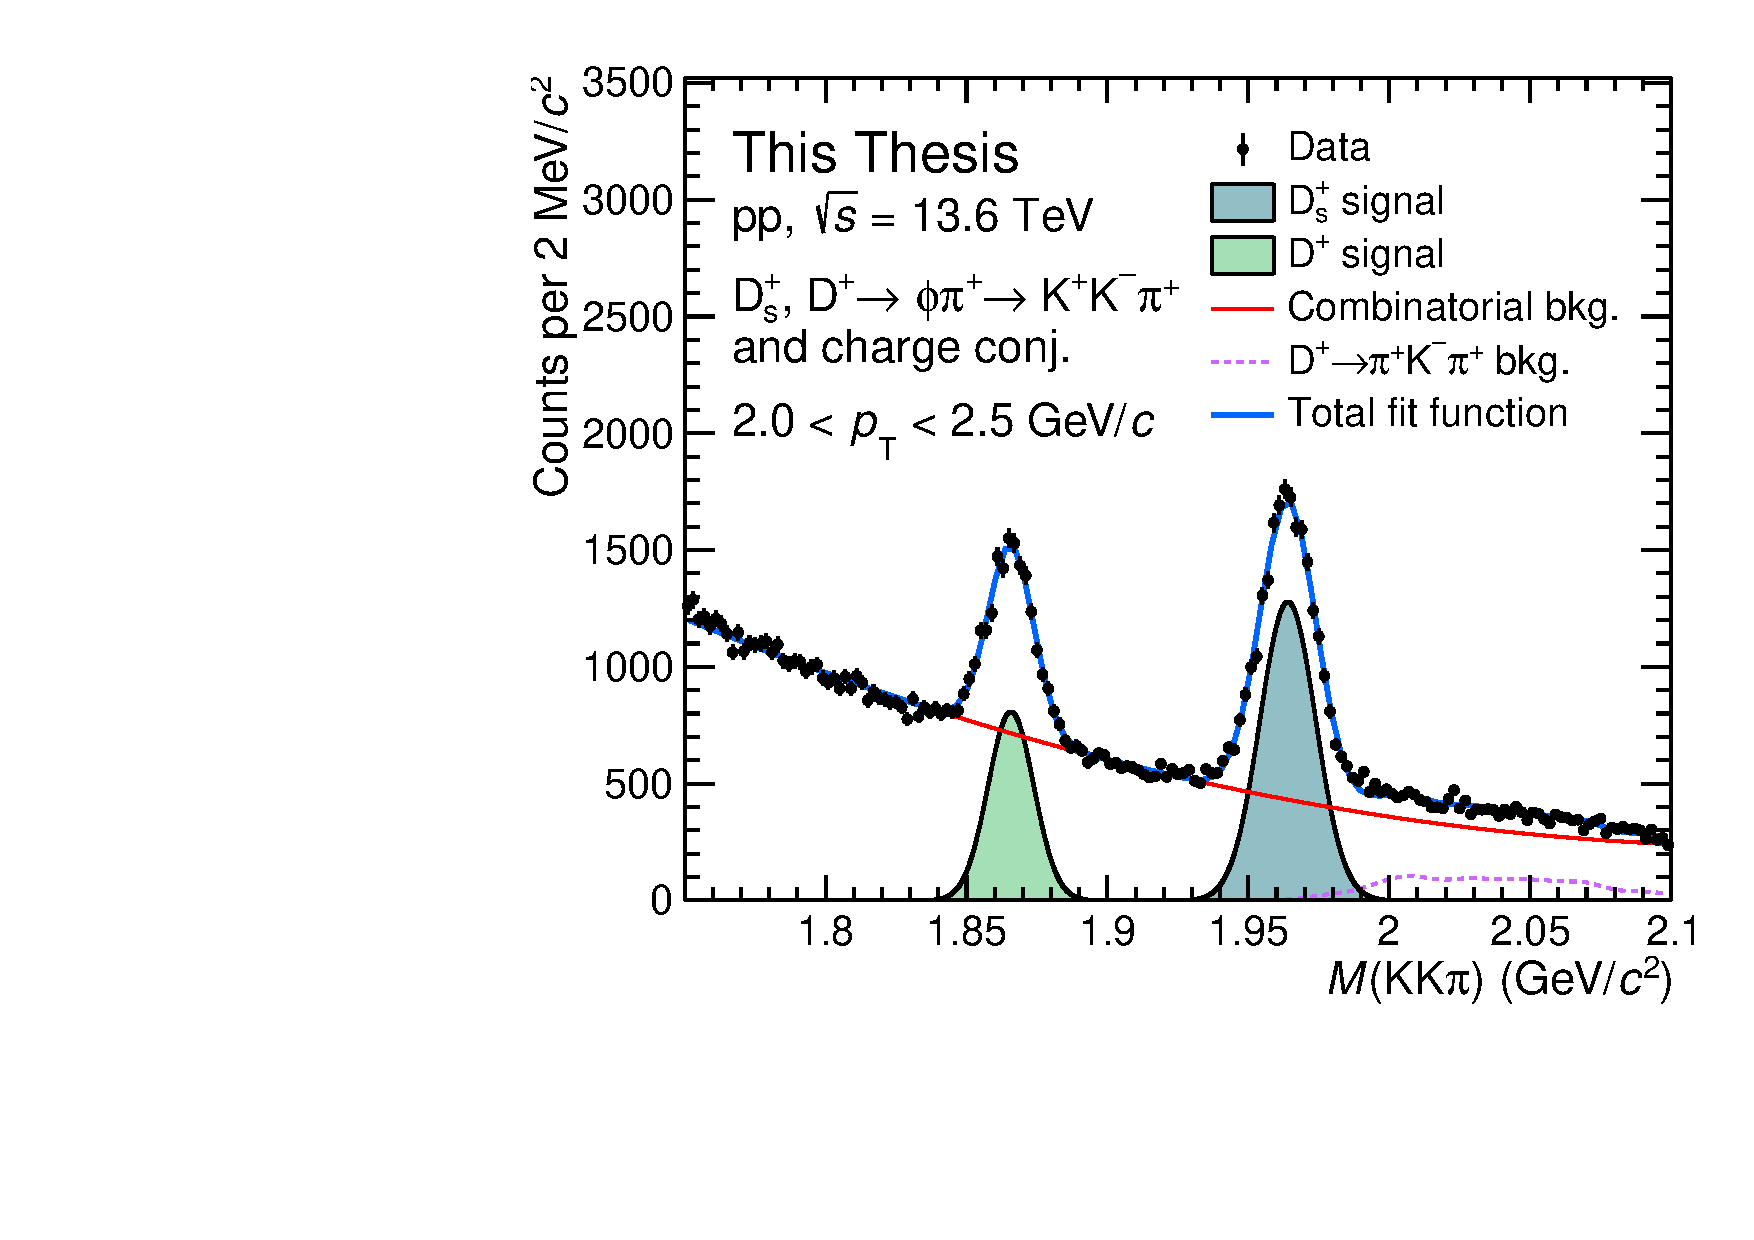
\includegraphics[width=0.2\textwidth]{Figures/Chapter 5/inv_mass/pt_2.0_2.5.pdf}
    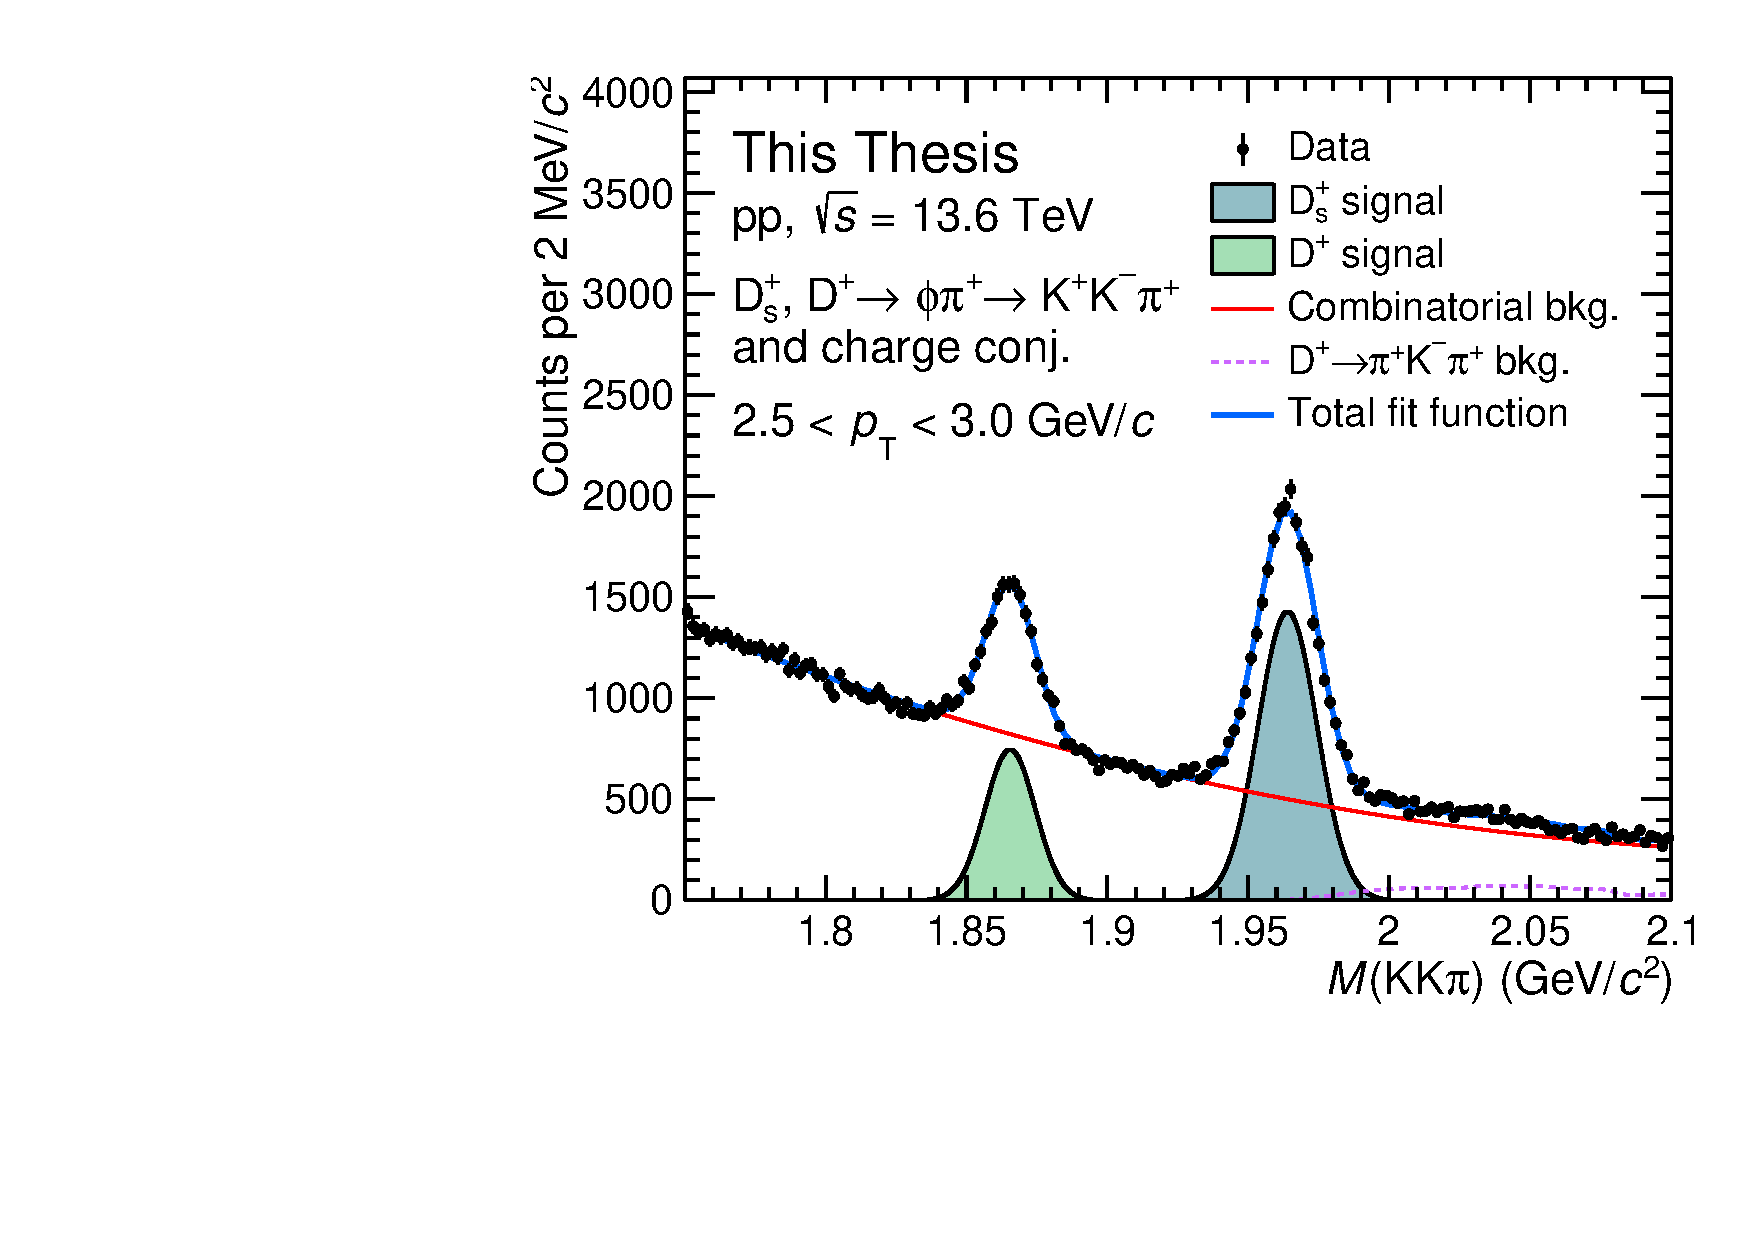
\includegraphics[width=0.2\textwidth]{Figures/Chapter 5/inv_mass/pt_2.5_3.0.pdf}
    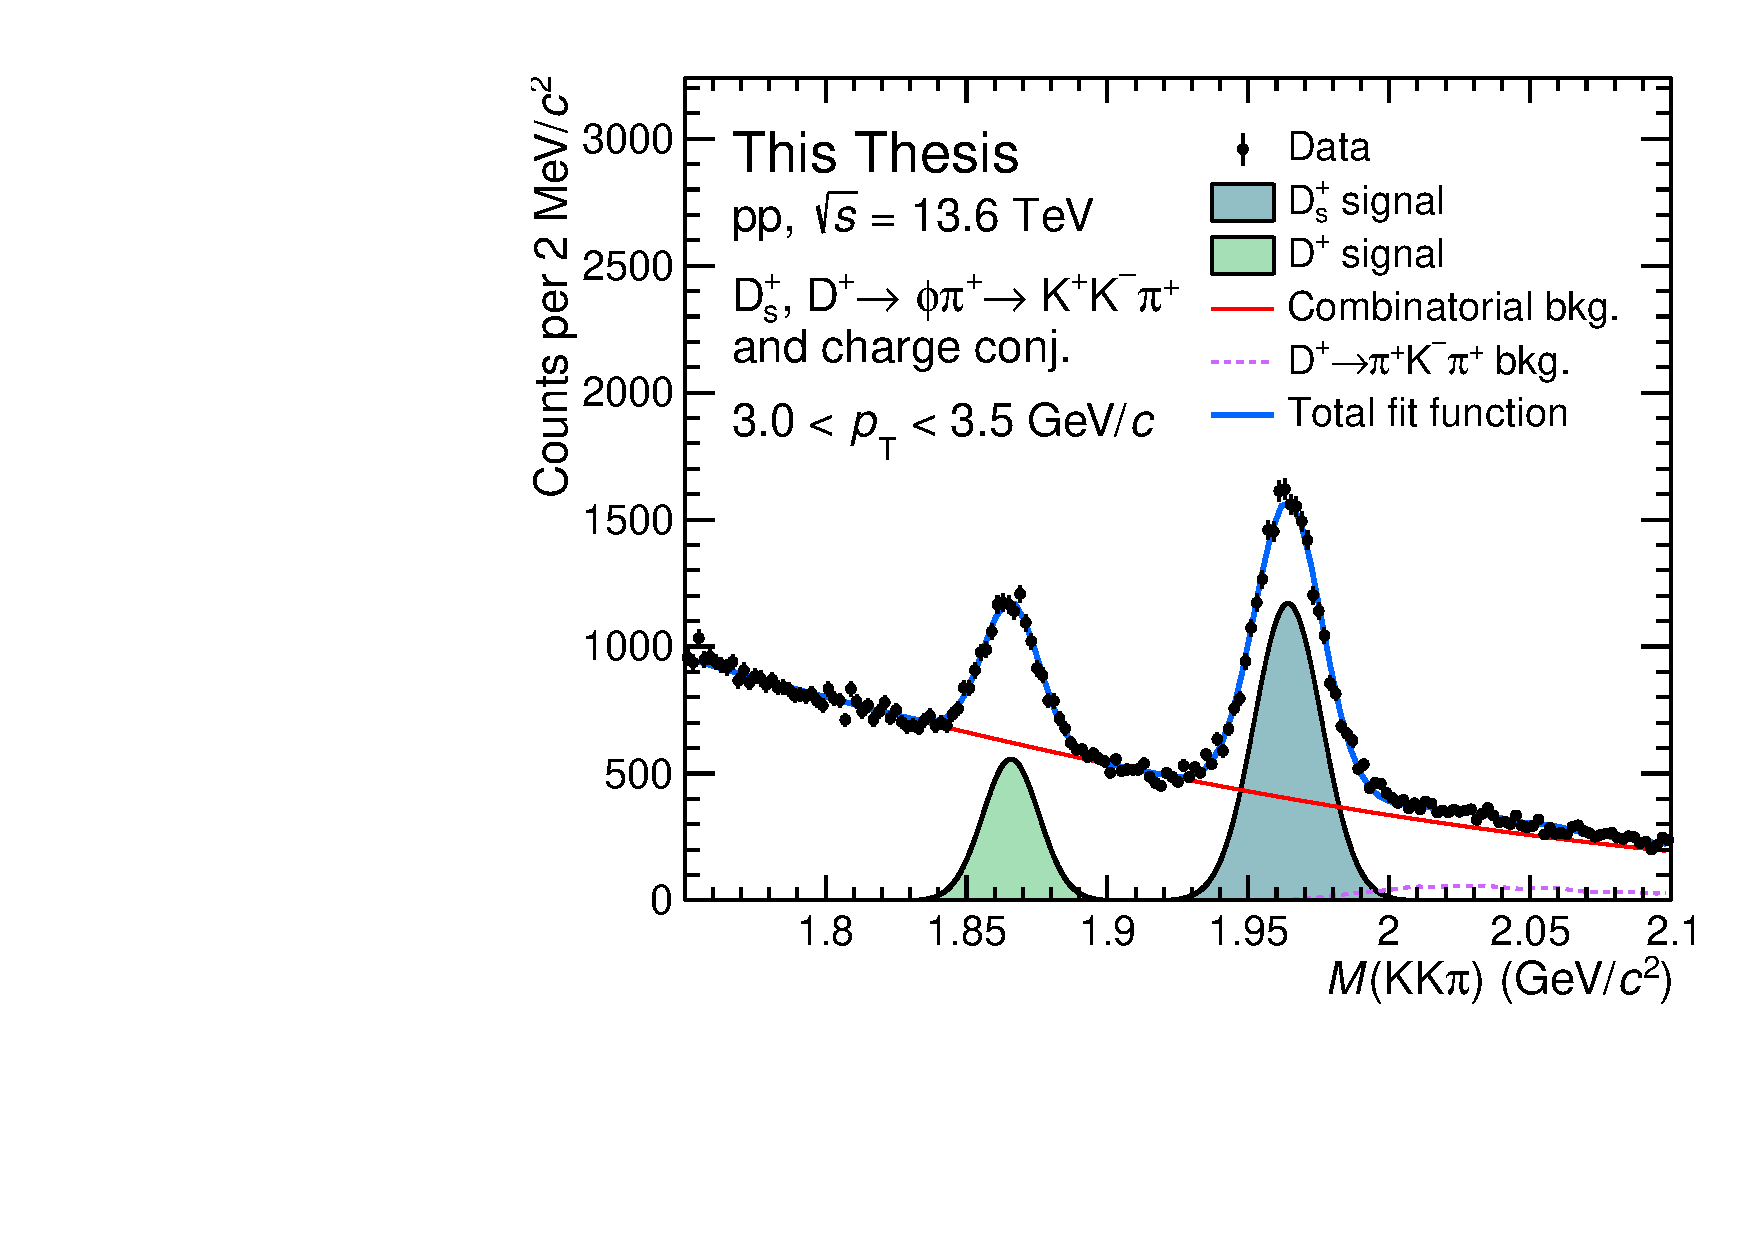
\includegraphics[width=0.2\textwidth]{Figures/Chapter 5/inv_mass/pt_3.0_3.5.pdf}
    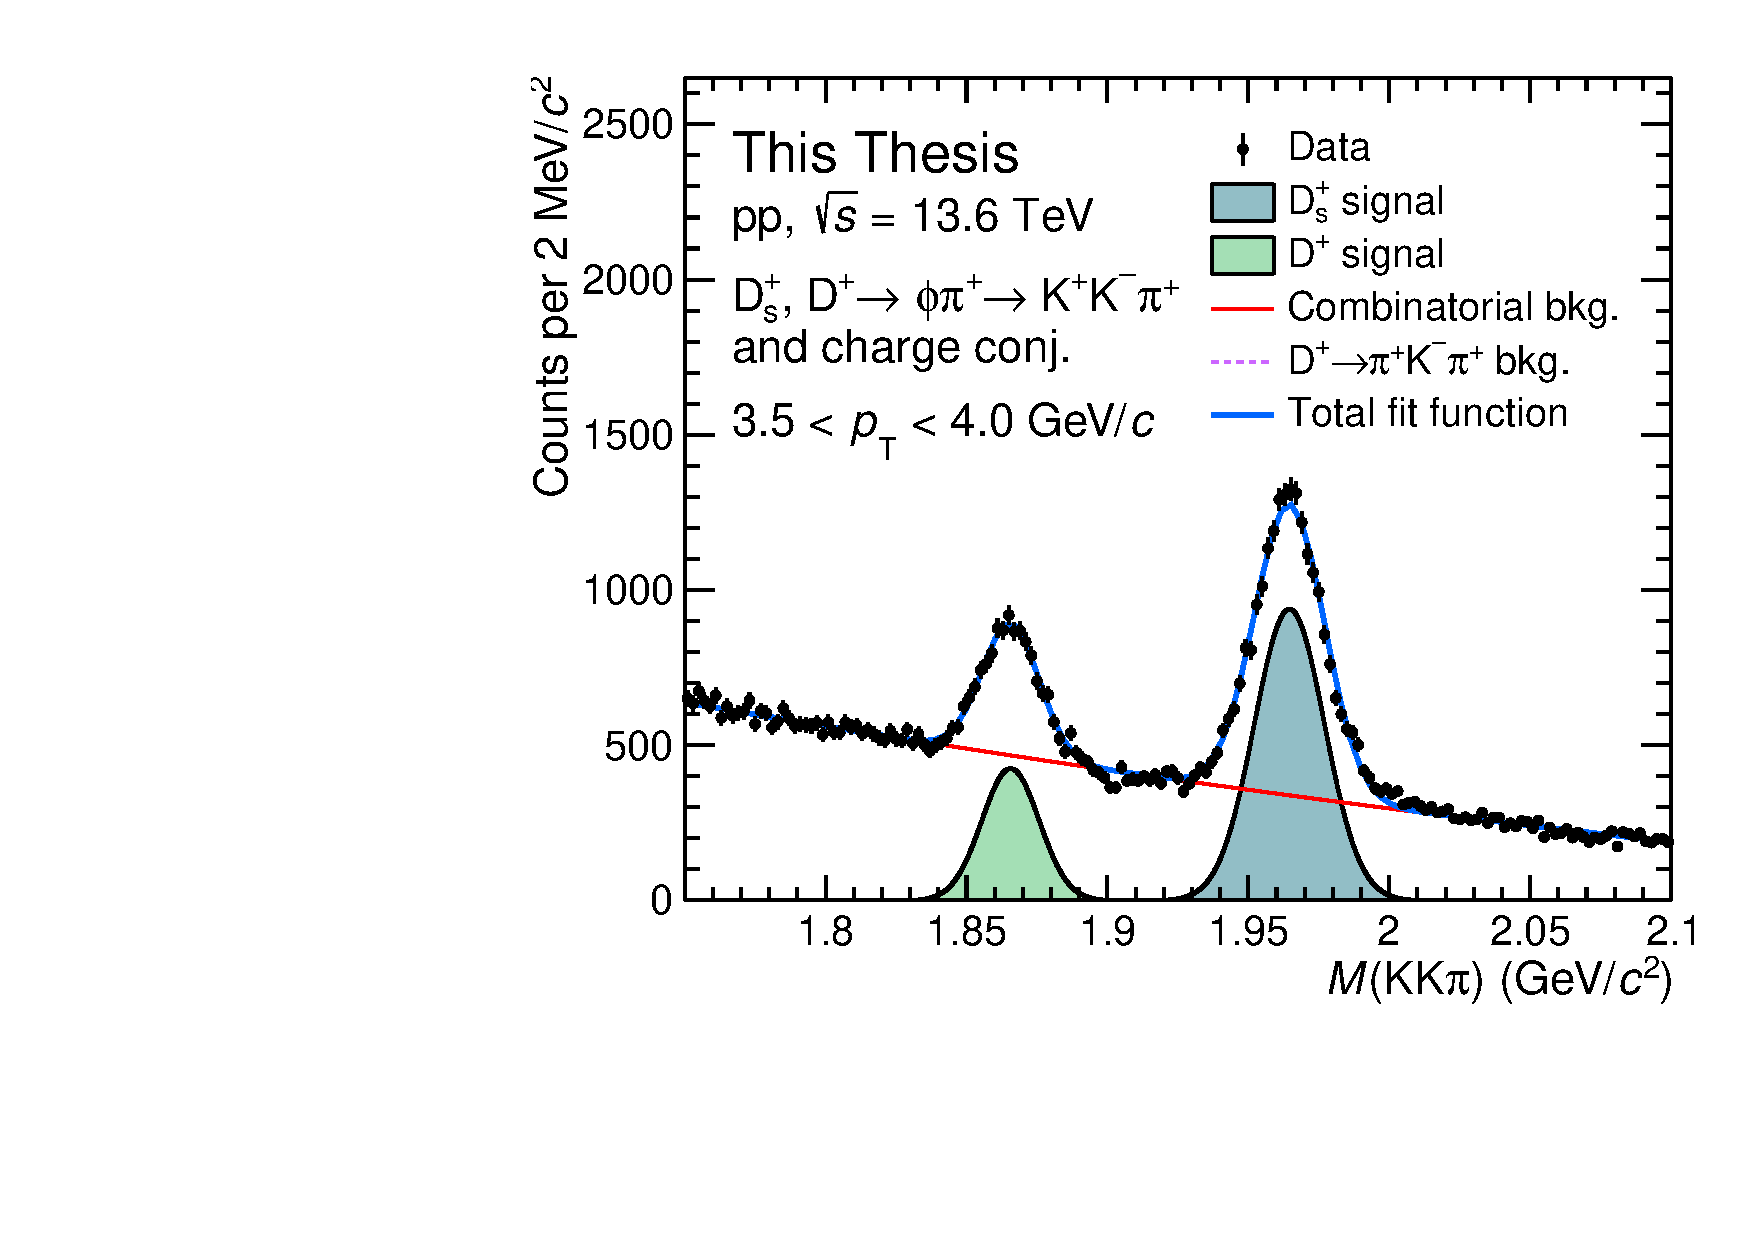
\includegraphics[width=0.2\textwidth]{Figures/Chapter 5/inv_mass/pt_3.5_4.0.pdf}
    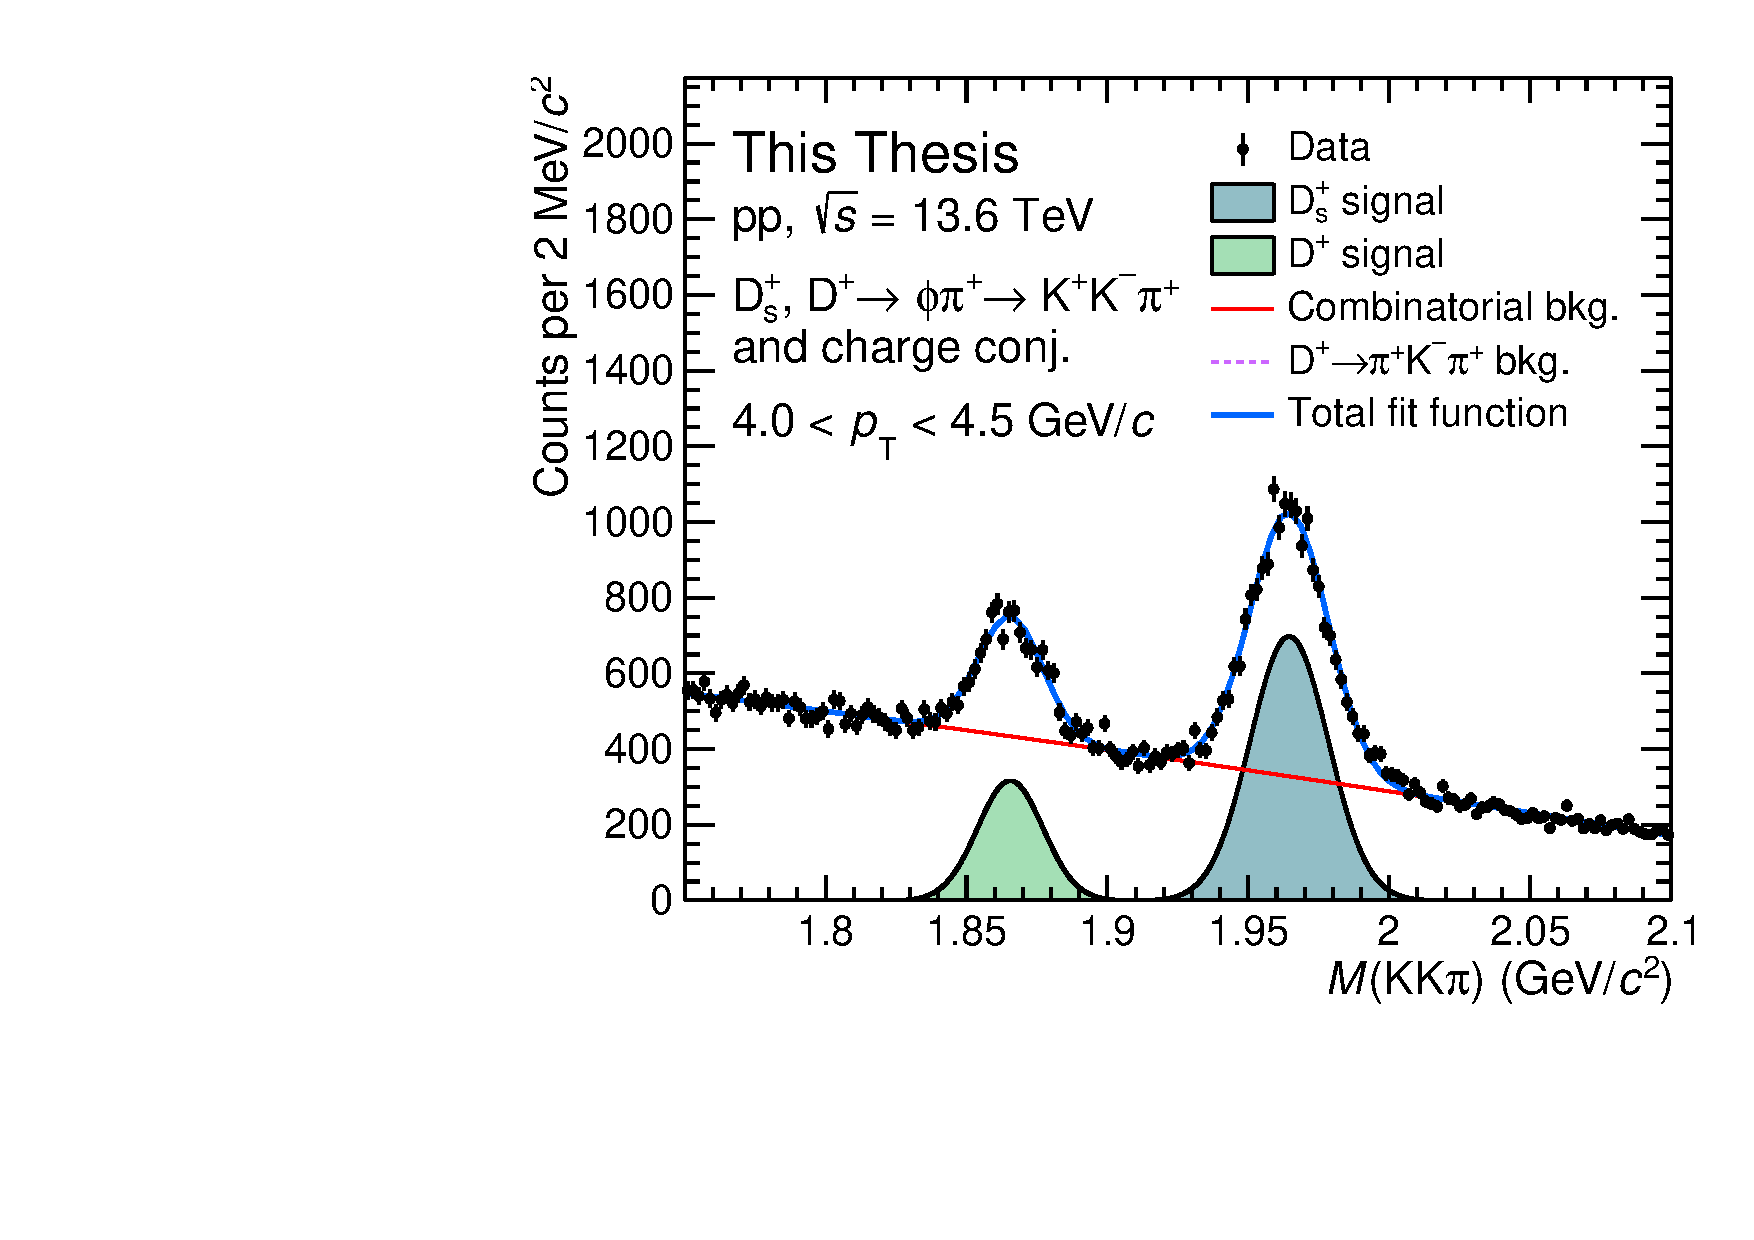
\includegraphics[width=0.2\textwidth]{Figures/Chapter 5/inv_mass/pt_4.0_4.5.pdf}
    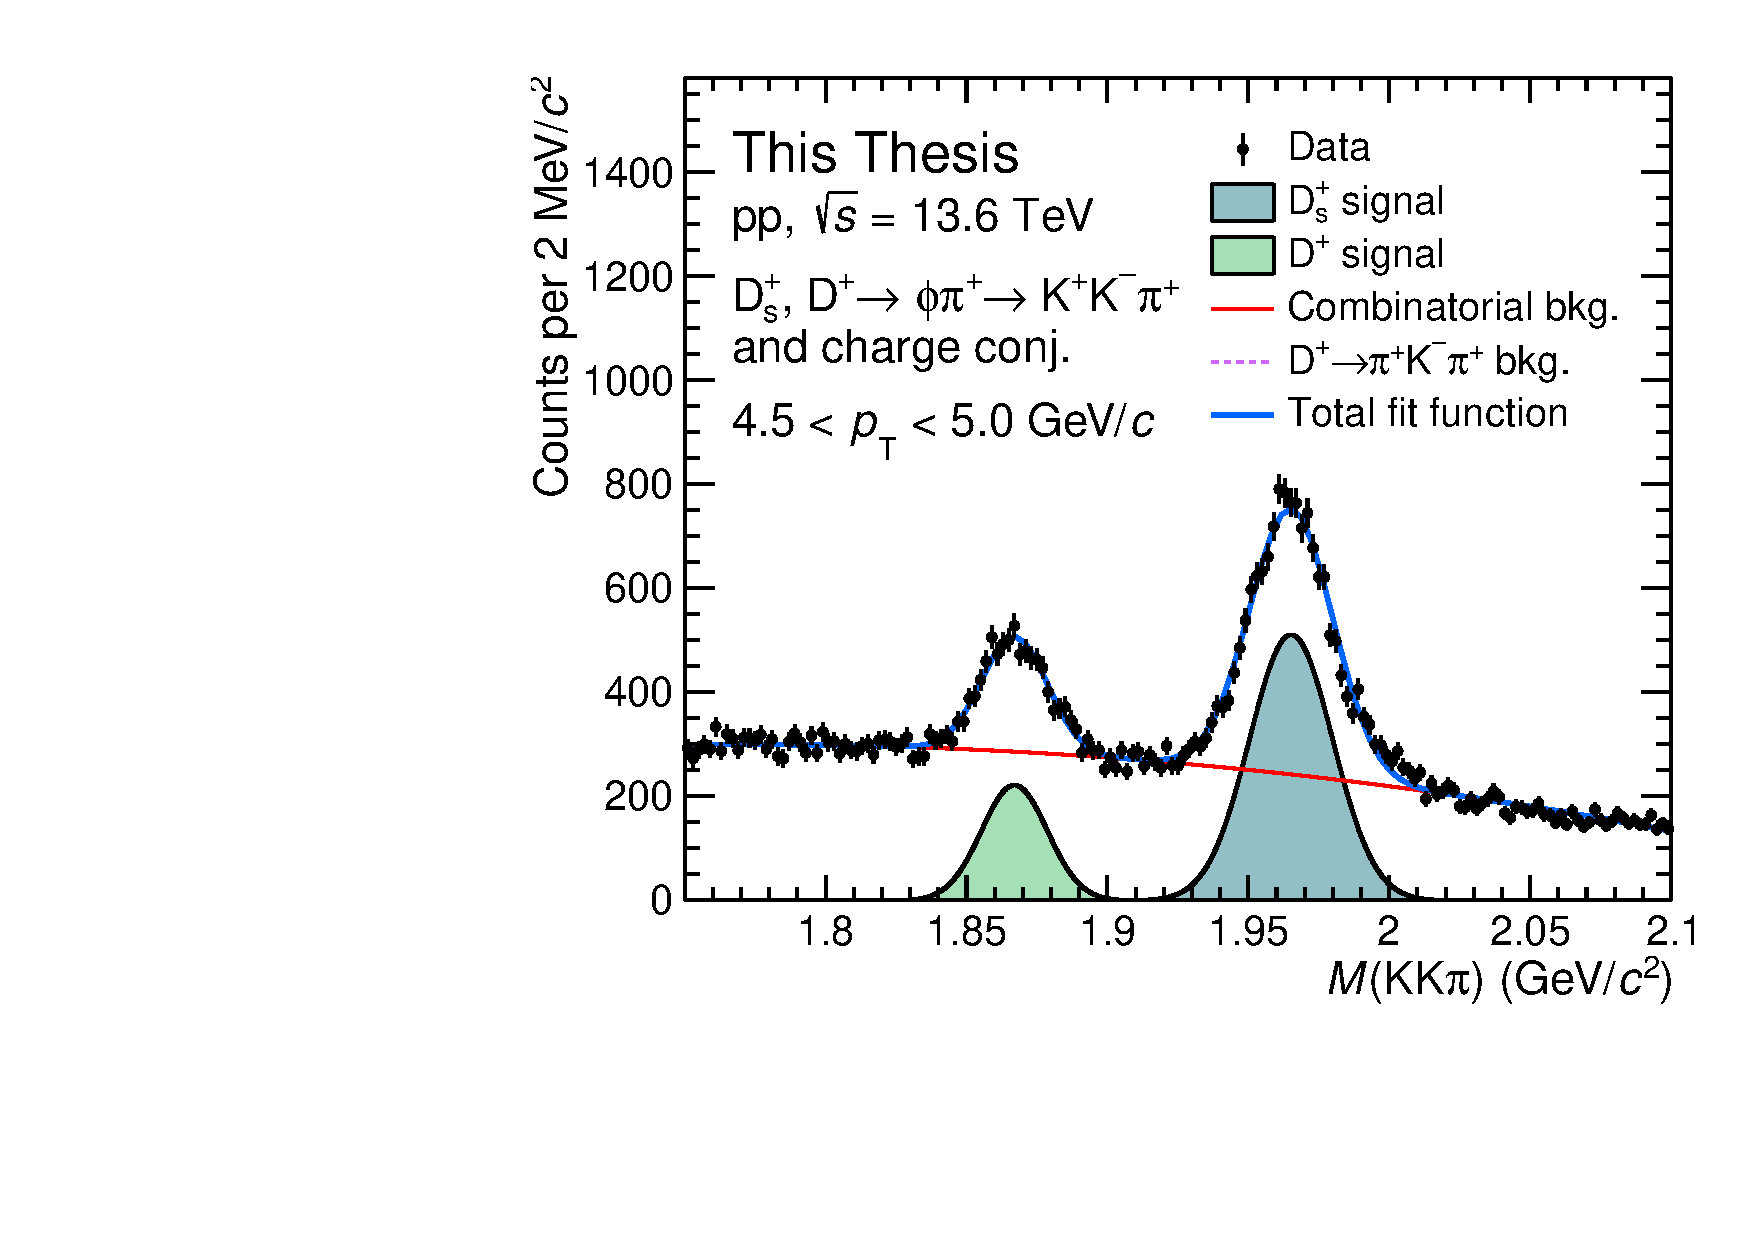
\includegraphics[width=0.2\textwidth]{Figures/Chapter 5/inv_mass/pt_4.5_5.0.pdf}
    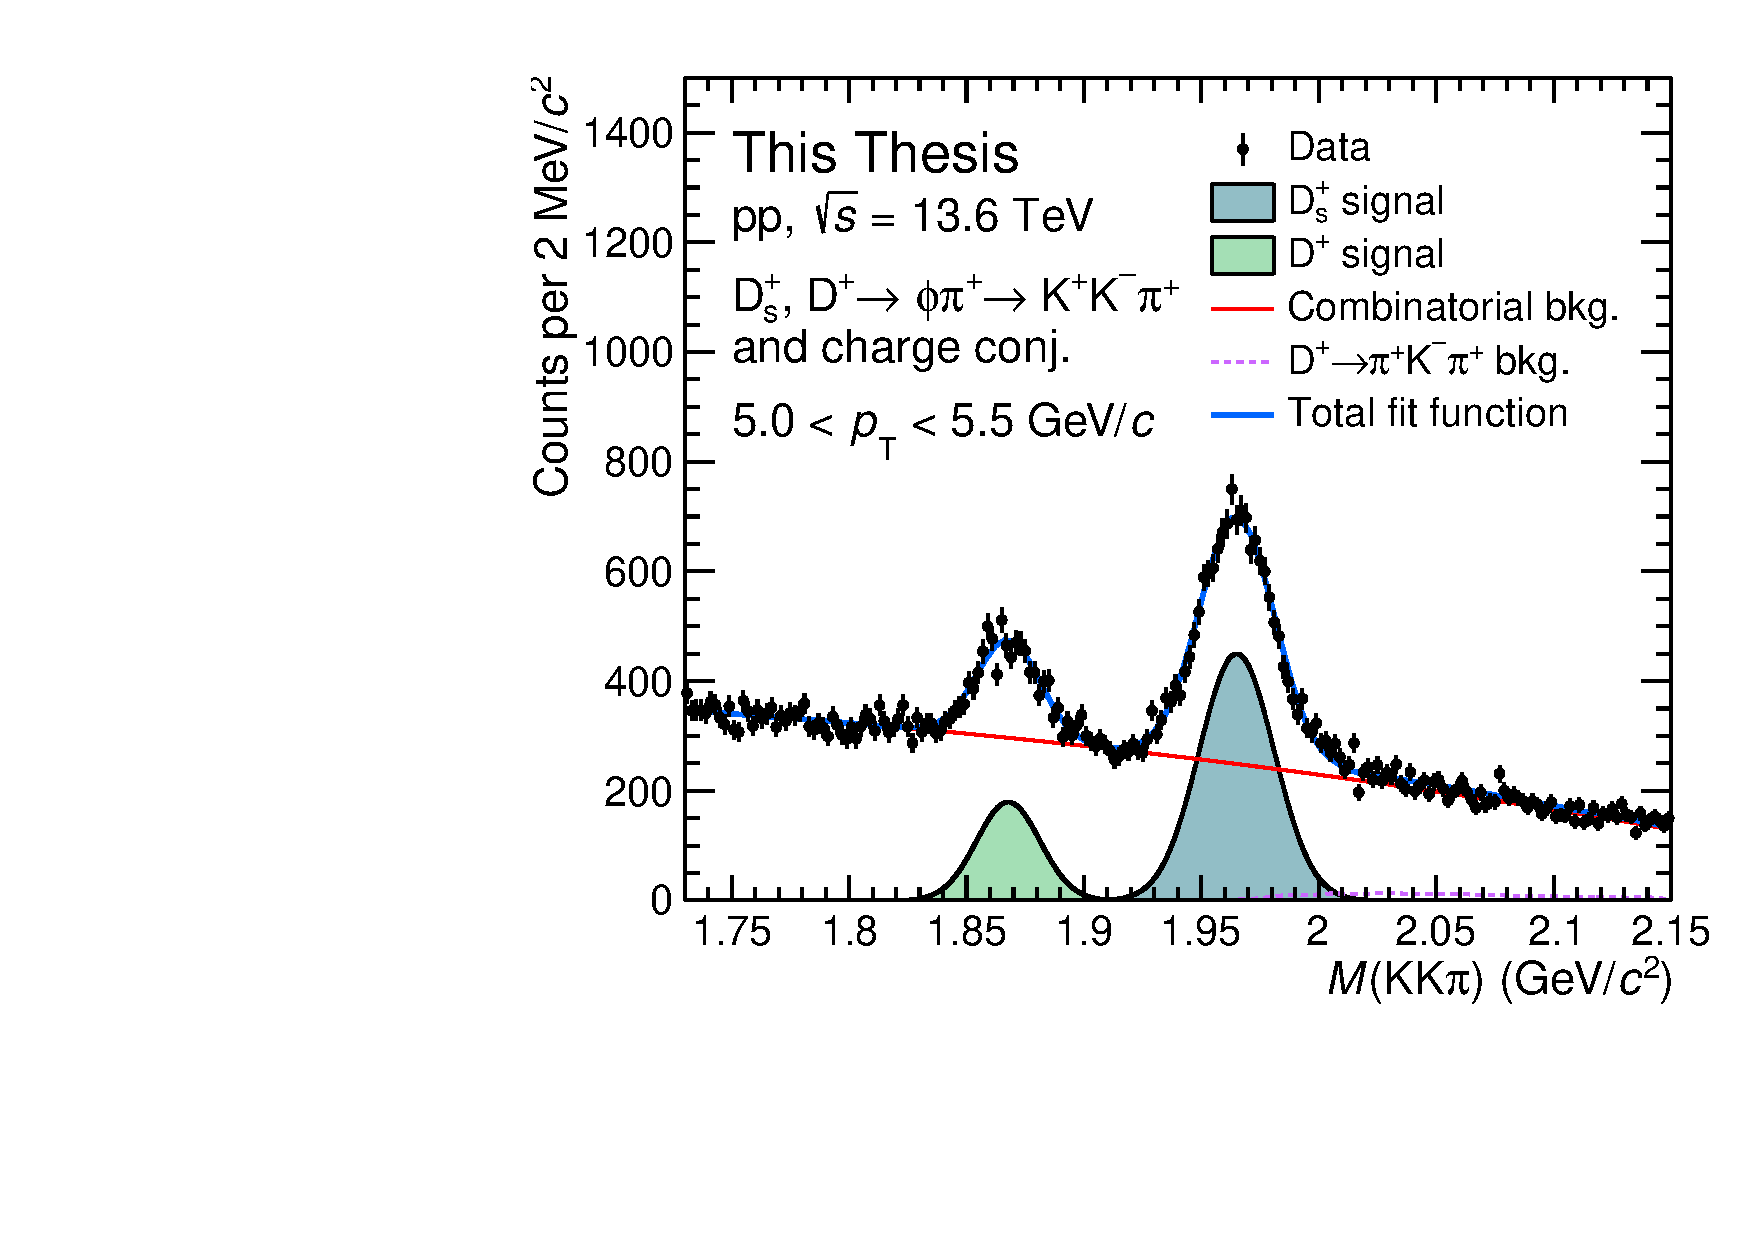
\includegraphics[width=0.2\textwidth]{Figures/Chapter 5/inv_mass/pt_5.0_5.5.pdf}
    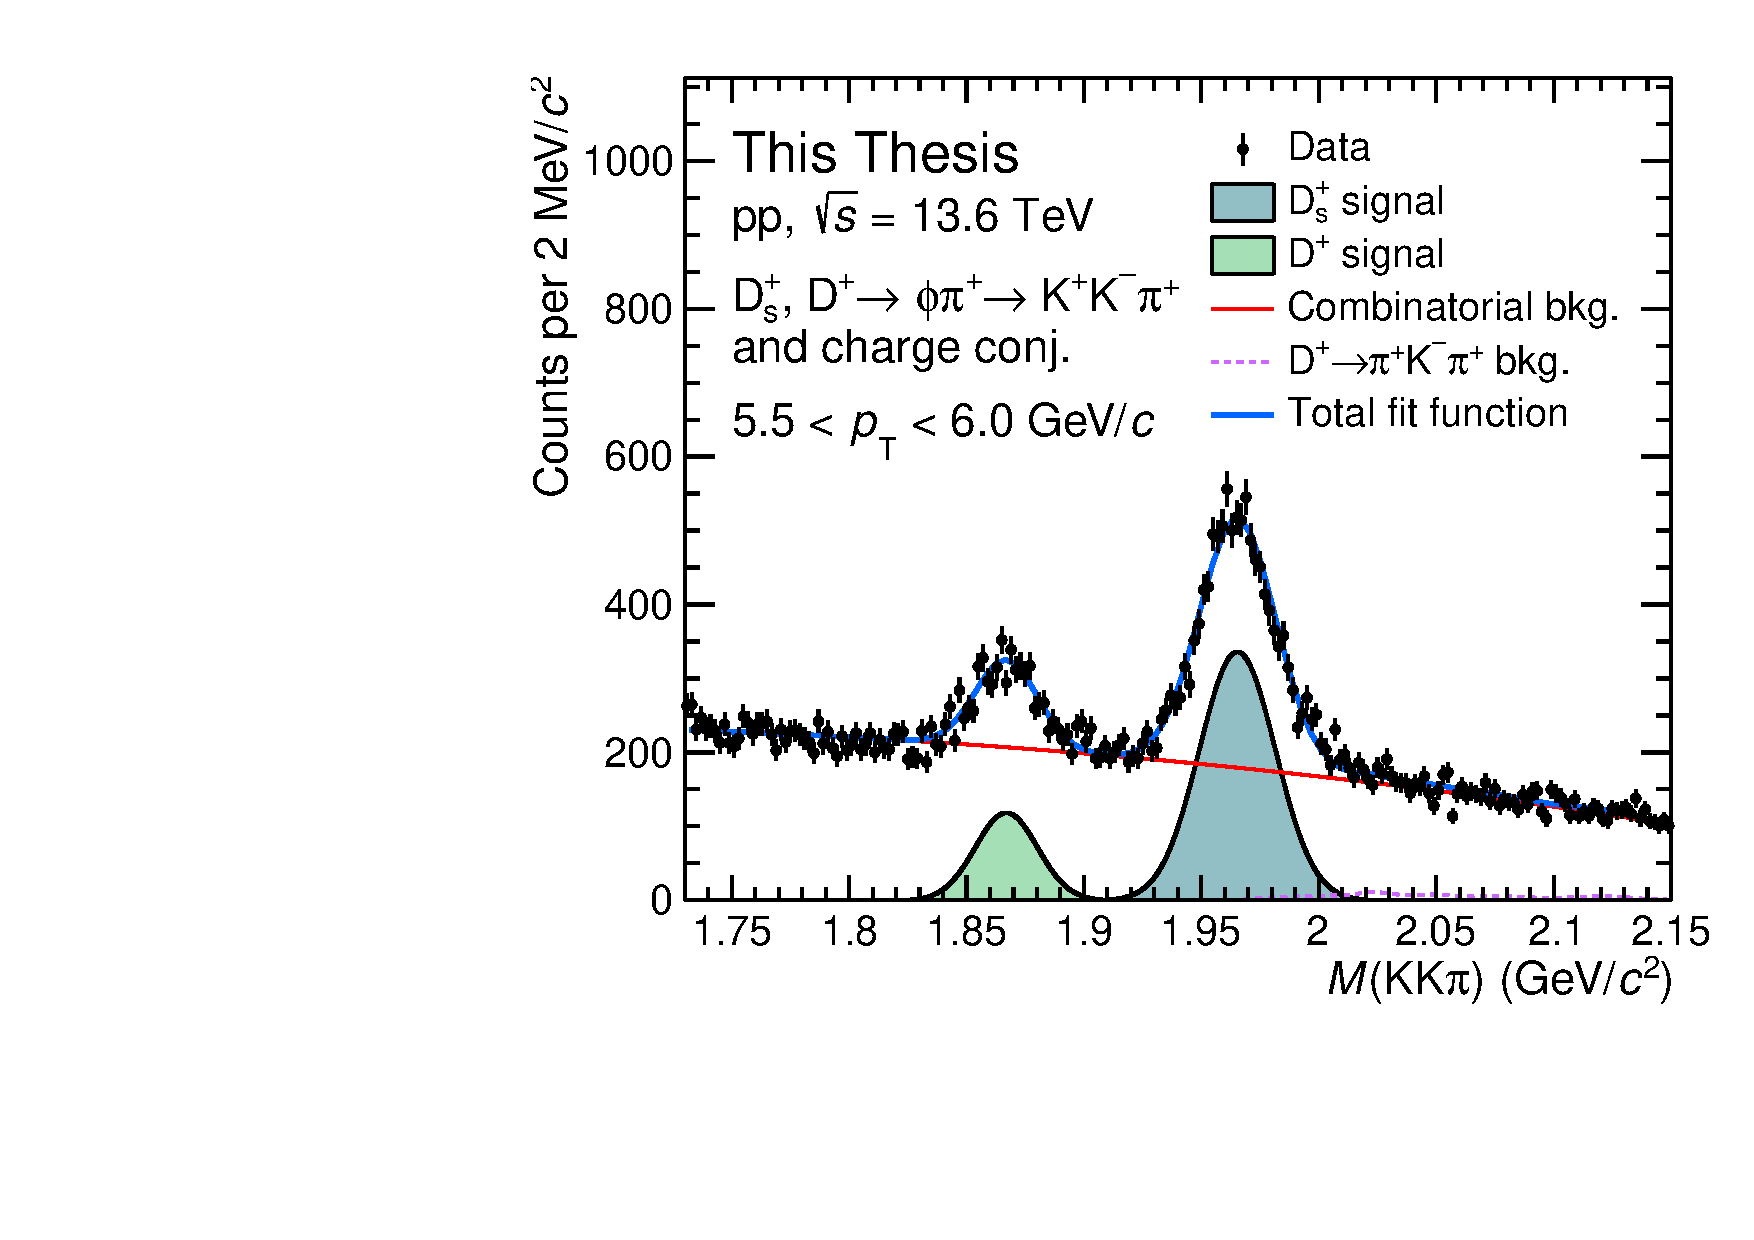
\includegraphics[width=0.2\textwidth]{Figures/Chapter 5/inv_mass/pt_5.5_6.0.pdf}
    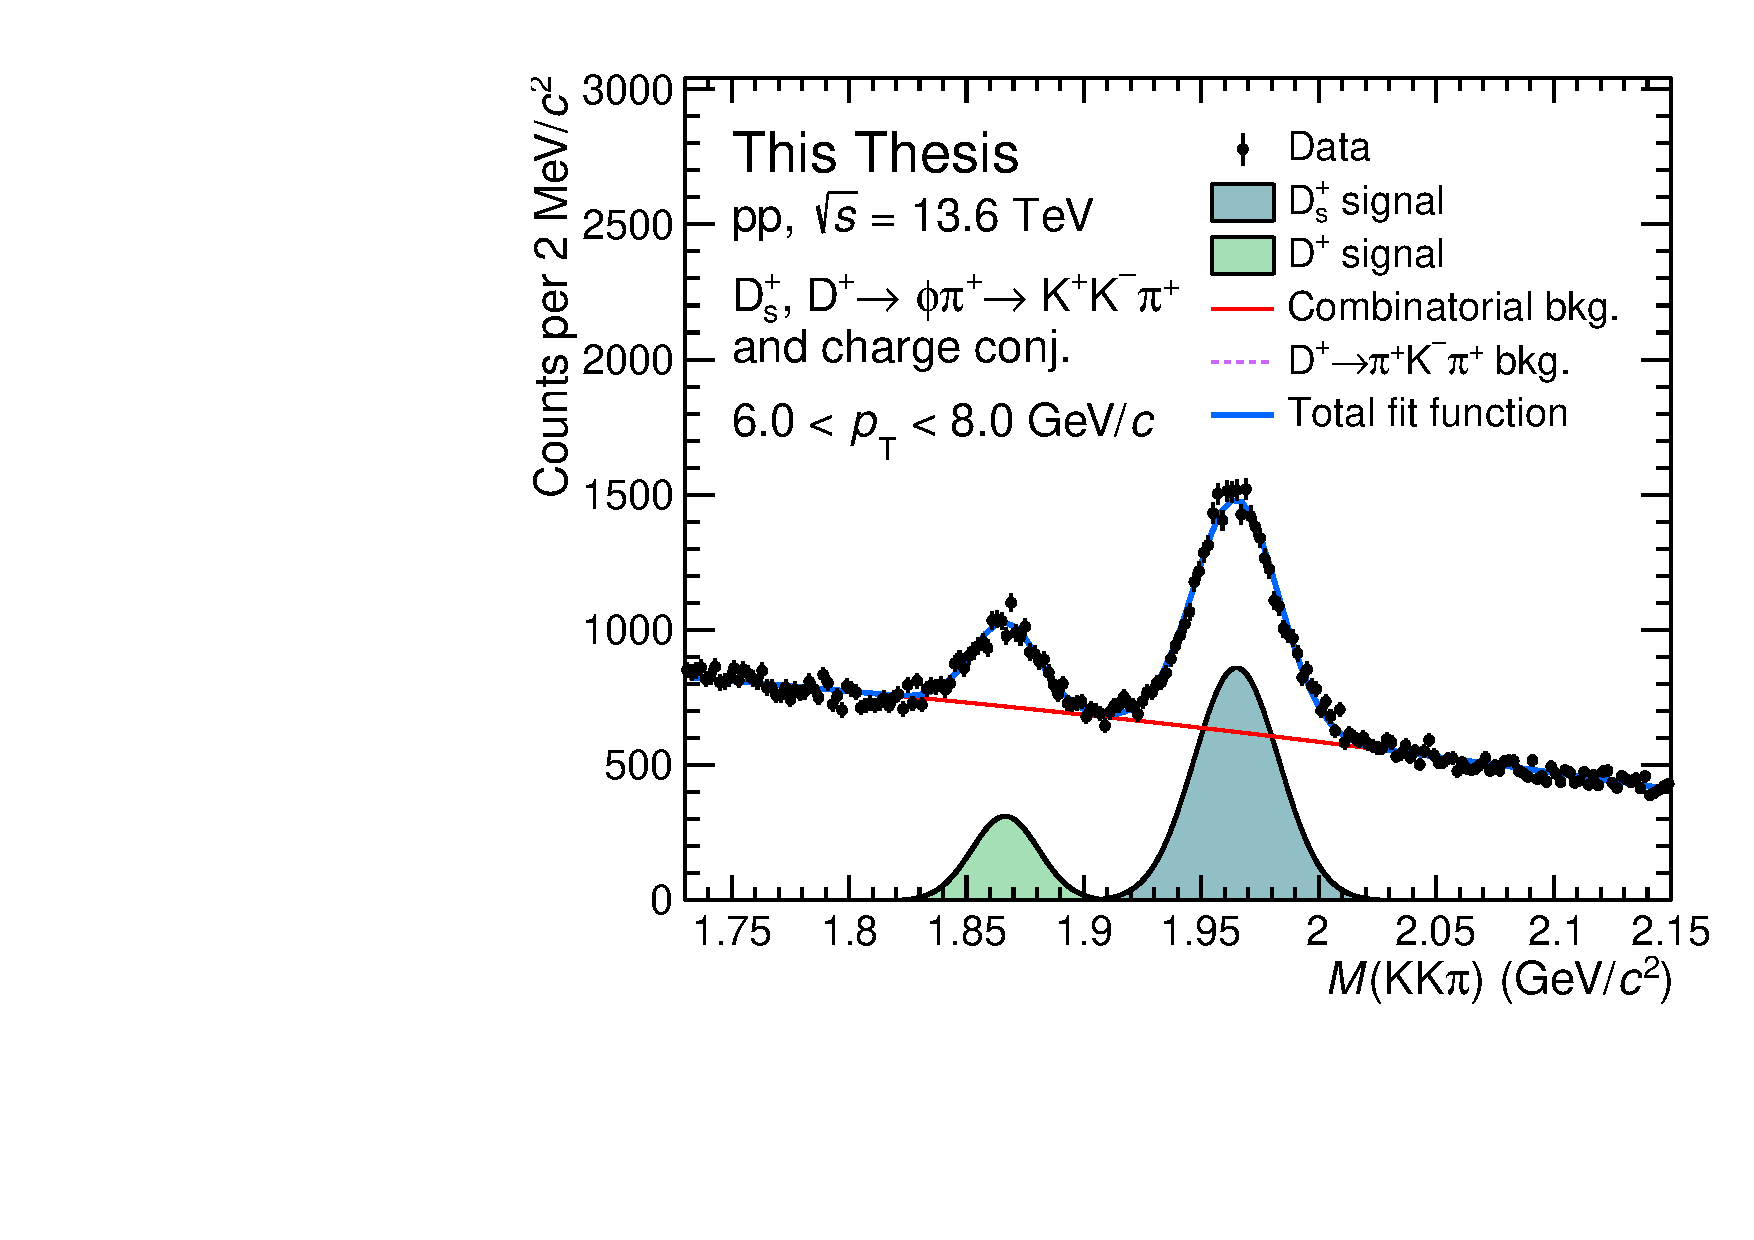
\includegraphics[width=0.2\textwidth]{Figures/Chapter 5/inv_mass/pt_6.0_8.0.pdf}
    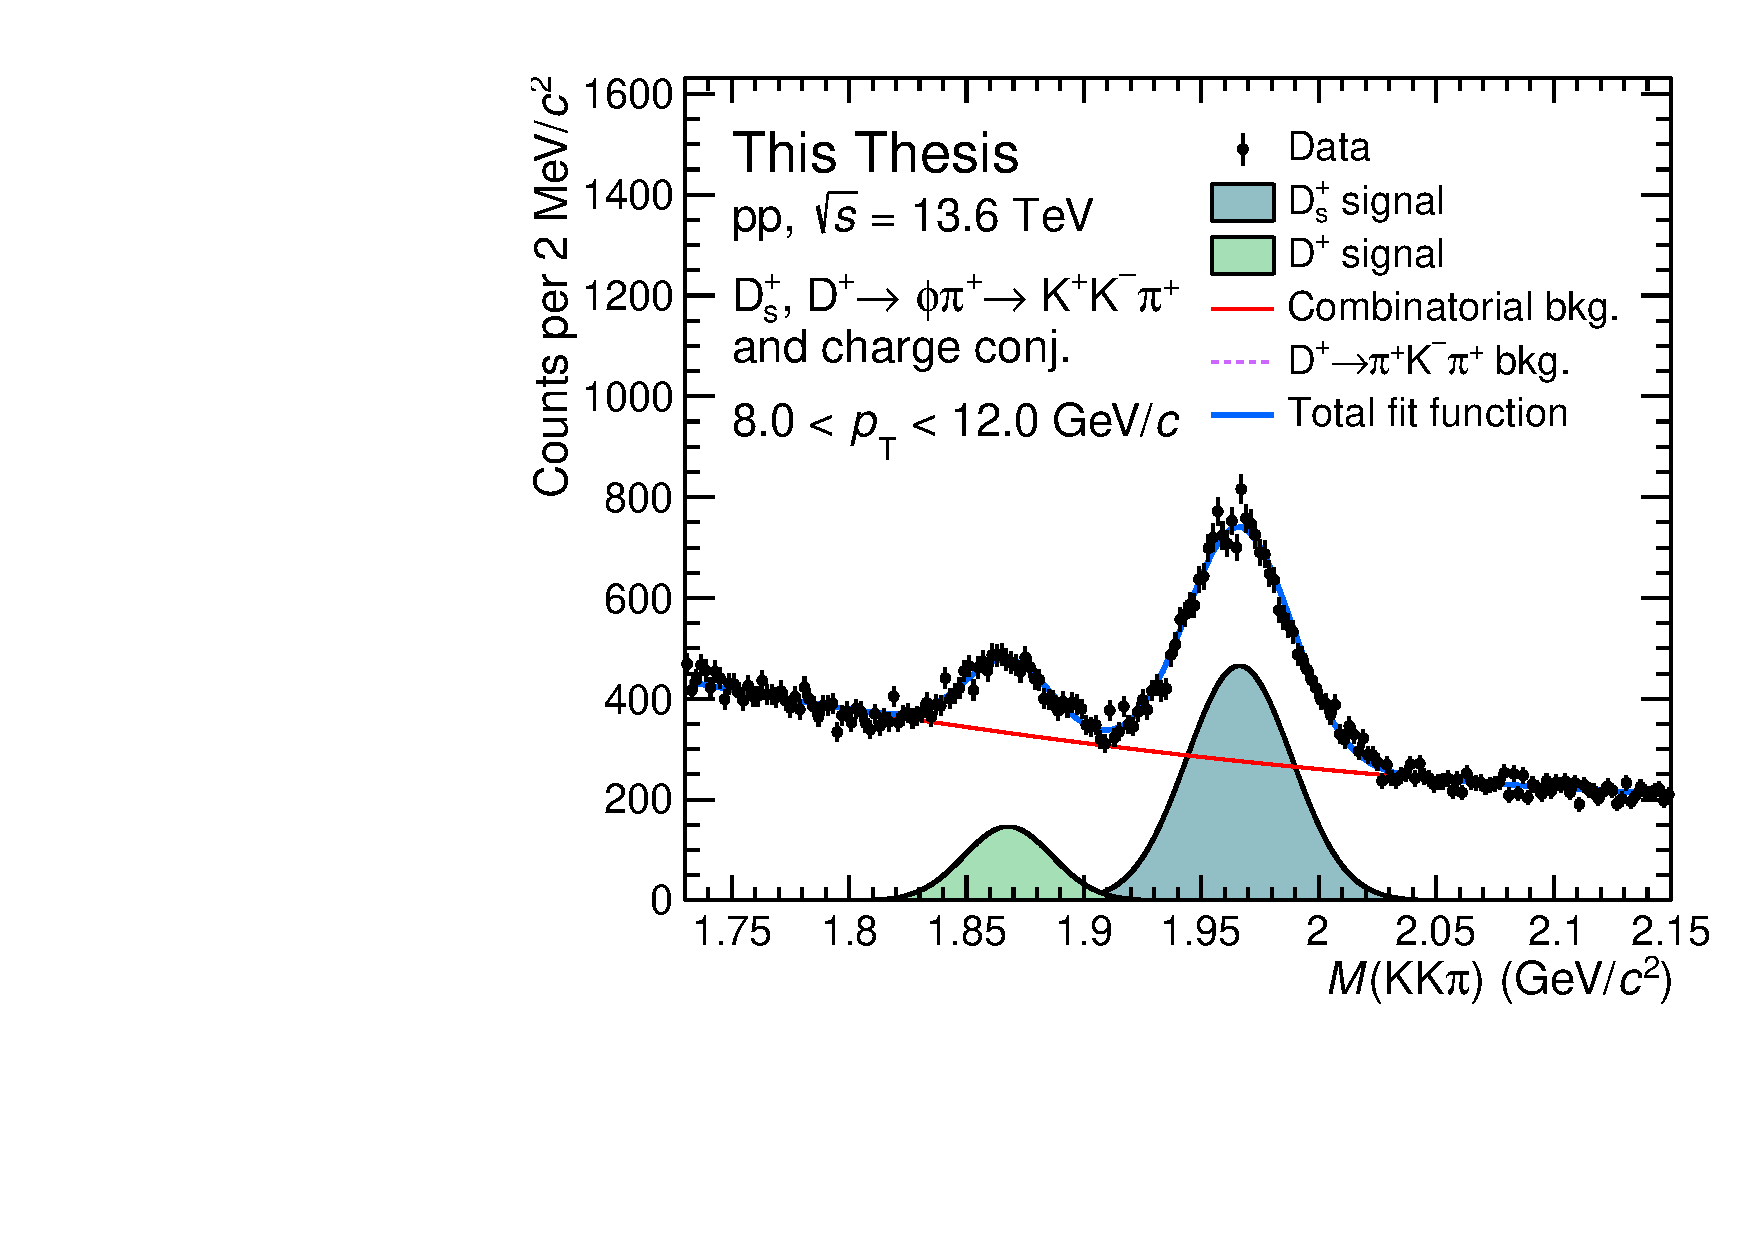
\includegraphics[width=0.2\textwidth]{Figures/Chapter 5/inv_mass/pt_8.0_12.0.pdf}
    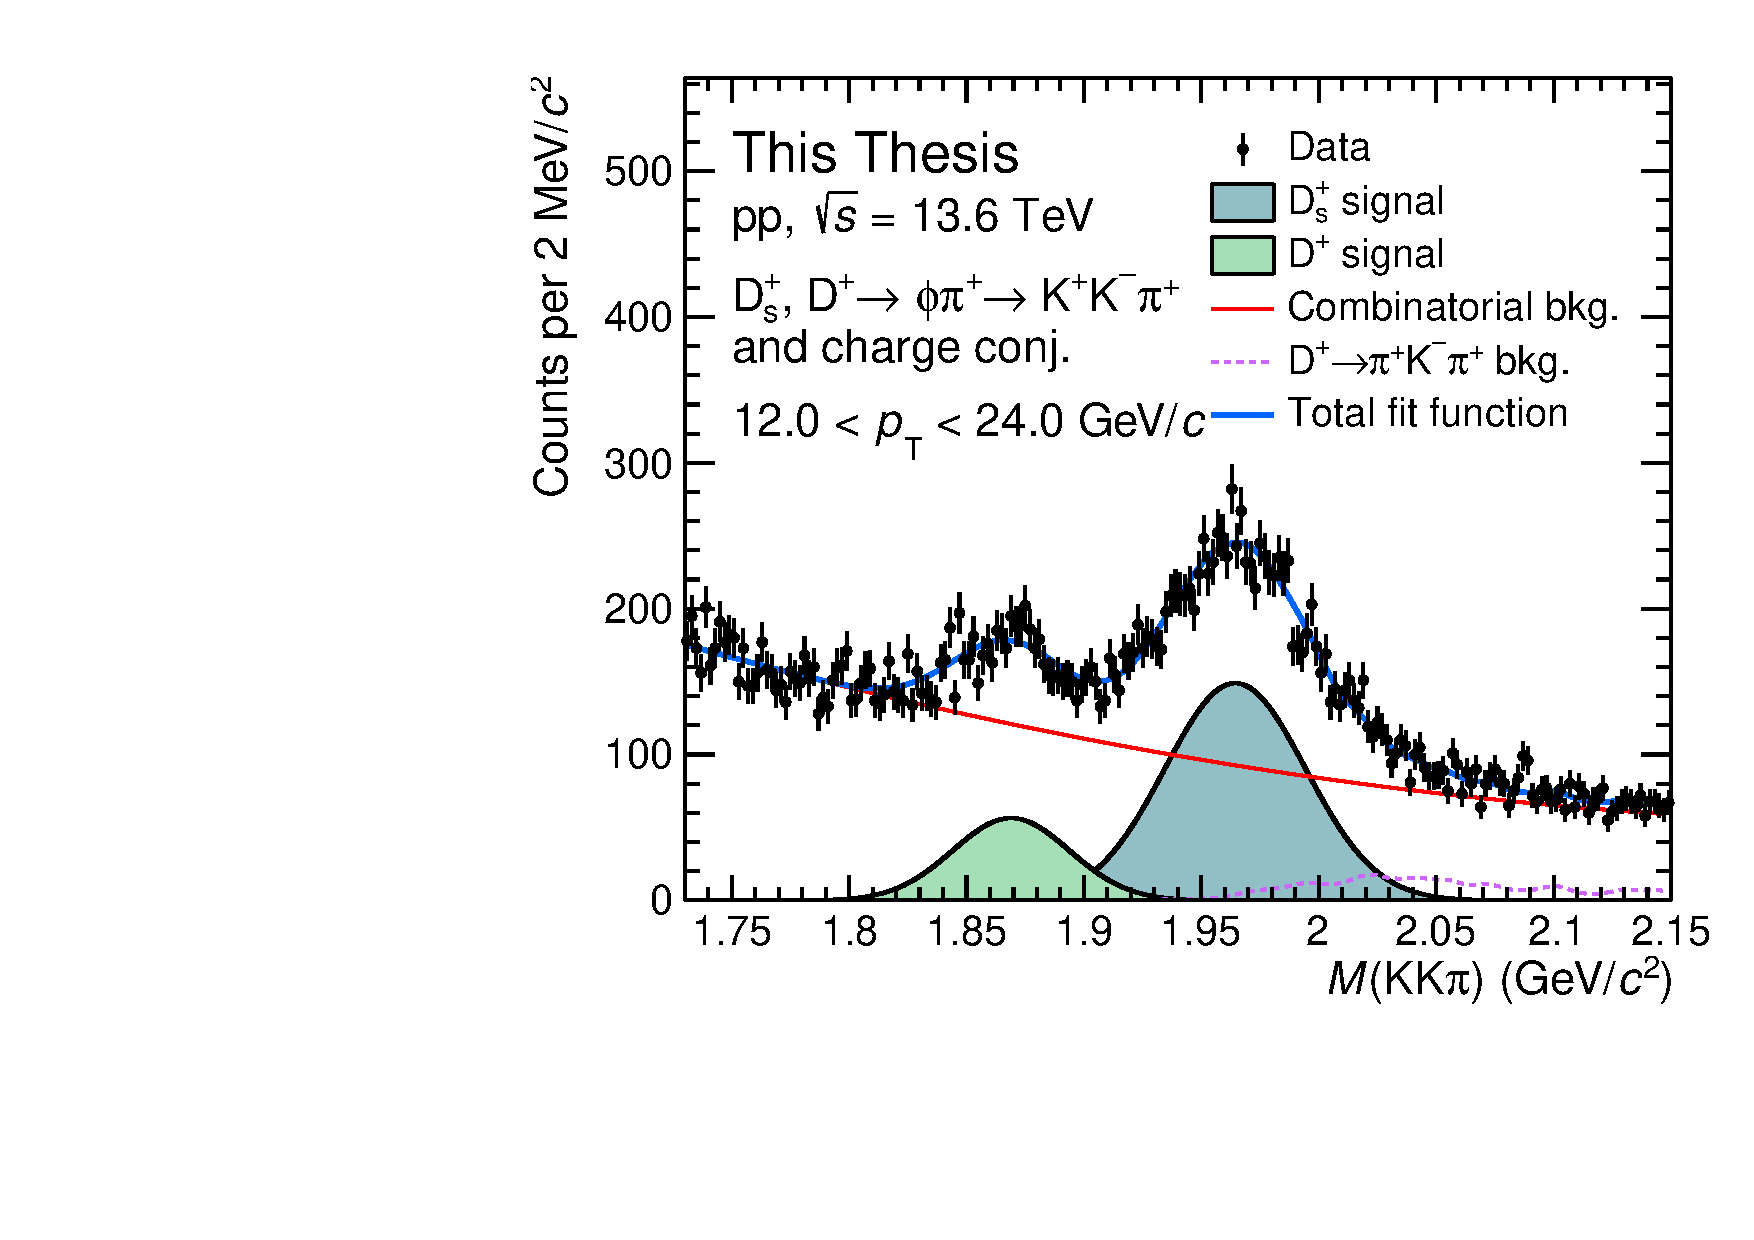
\includegraphics[width=0.2\textwidth]{Figures/Chapter 5/inv_mass/pt_12.0_24.0.pdf}
    \caption{Fit to the invariant mass distribution of selected candidate in the 14 studied \pt intervals in the \mbox{$0.5<\pt<24$~\gevc} range. The total fit function is shown as a solid blue line, while background components are shown as solid red lines (correlated background) and dashed violet lines (dashed violet lines). The signal contributions are shown as filled green and azure areas for \dpl and \ds mesons, respectively.}
    \label{fig:new_fit_all}
\end{sidewaysfigure}

The evolution of the mean and width of the \ds and \dpl meson peaks as a function of \pt is shown in Fig.~\ref{fig:mean_width}. In the left panel, the means of the Gaussian functions used to describe the \ds- and \dpl-meson peaks are shown as a function of \pt. They present an increasing trend with \pt lying below the values reported in the PDG~\cite{pdg}, represented with dashed lines. The shift of the mass values observed in data from those reported in the PDG is common to all analyses of D mesons due to an imperfect description of the detector misalignments in MC simulations. In the right panel, the peak widths of the \ds and \dpl mesons, defined as the standard deviation of the Gaussian functions used to describe their invariant mass distributions, are shown as a function of \pt. An increasing trend with \pt is observed for both mesons, as detailed above for Fig.~\ref{fig:sigma_ratio}, with the peak width of the \ds meson being larger than that of the \dpl meson across the studied \pt range.

\begin{figure}[htb]
    \centering
    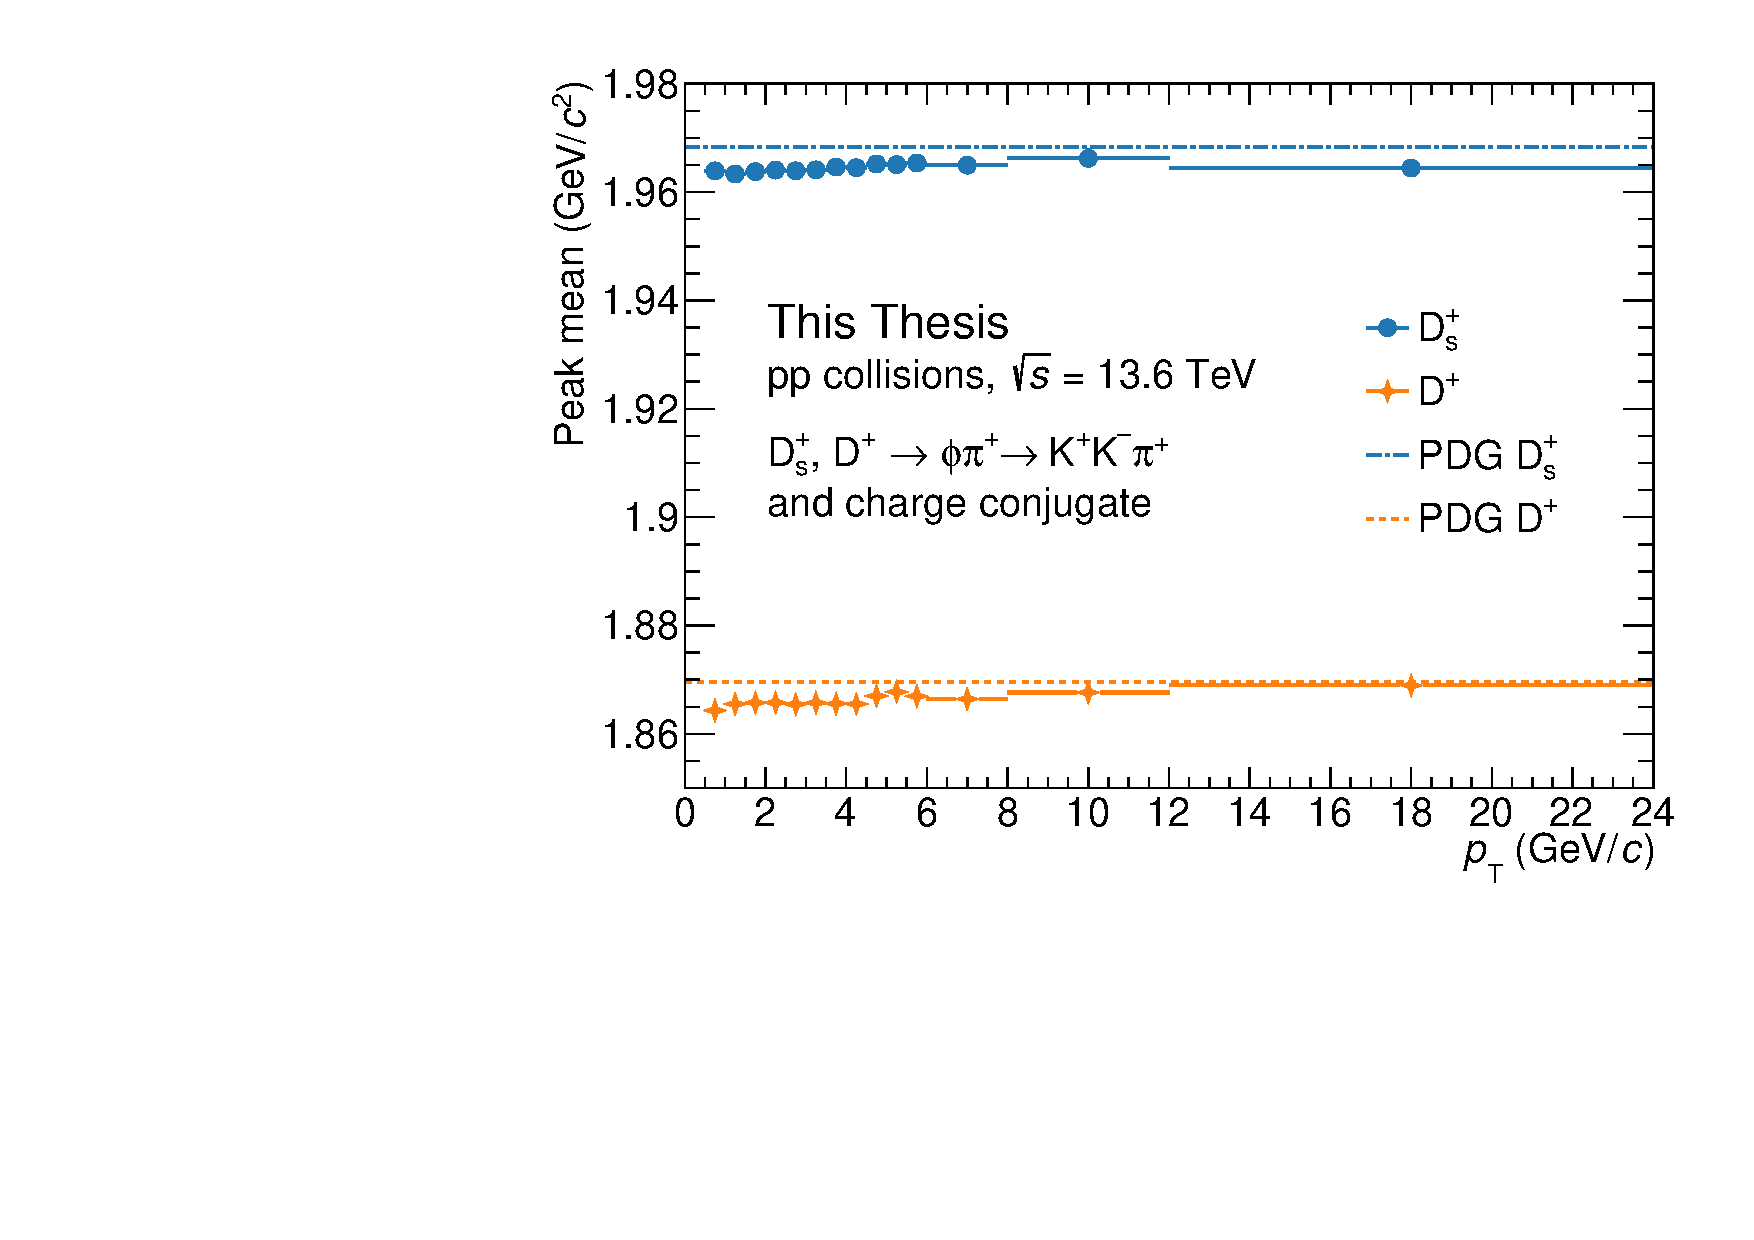
\includegraphics[width=0.48\textwidth]{Figures/Chapter 5/Mean.pdf}
    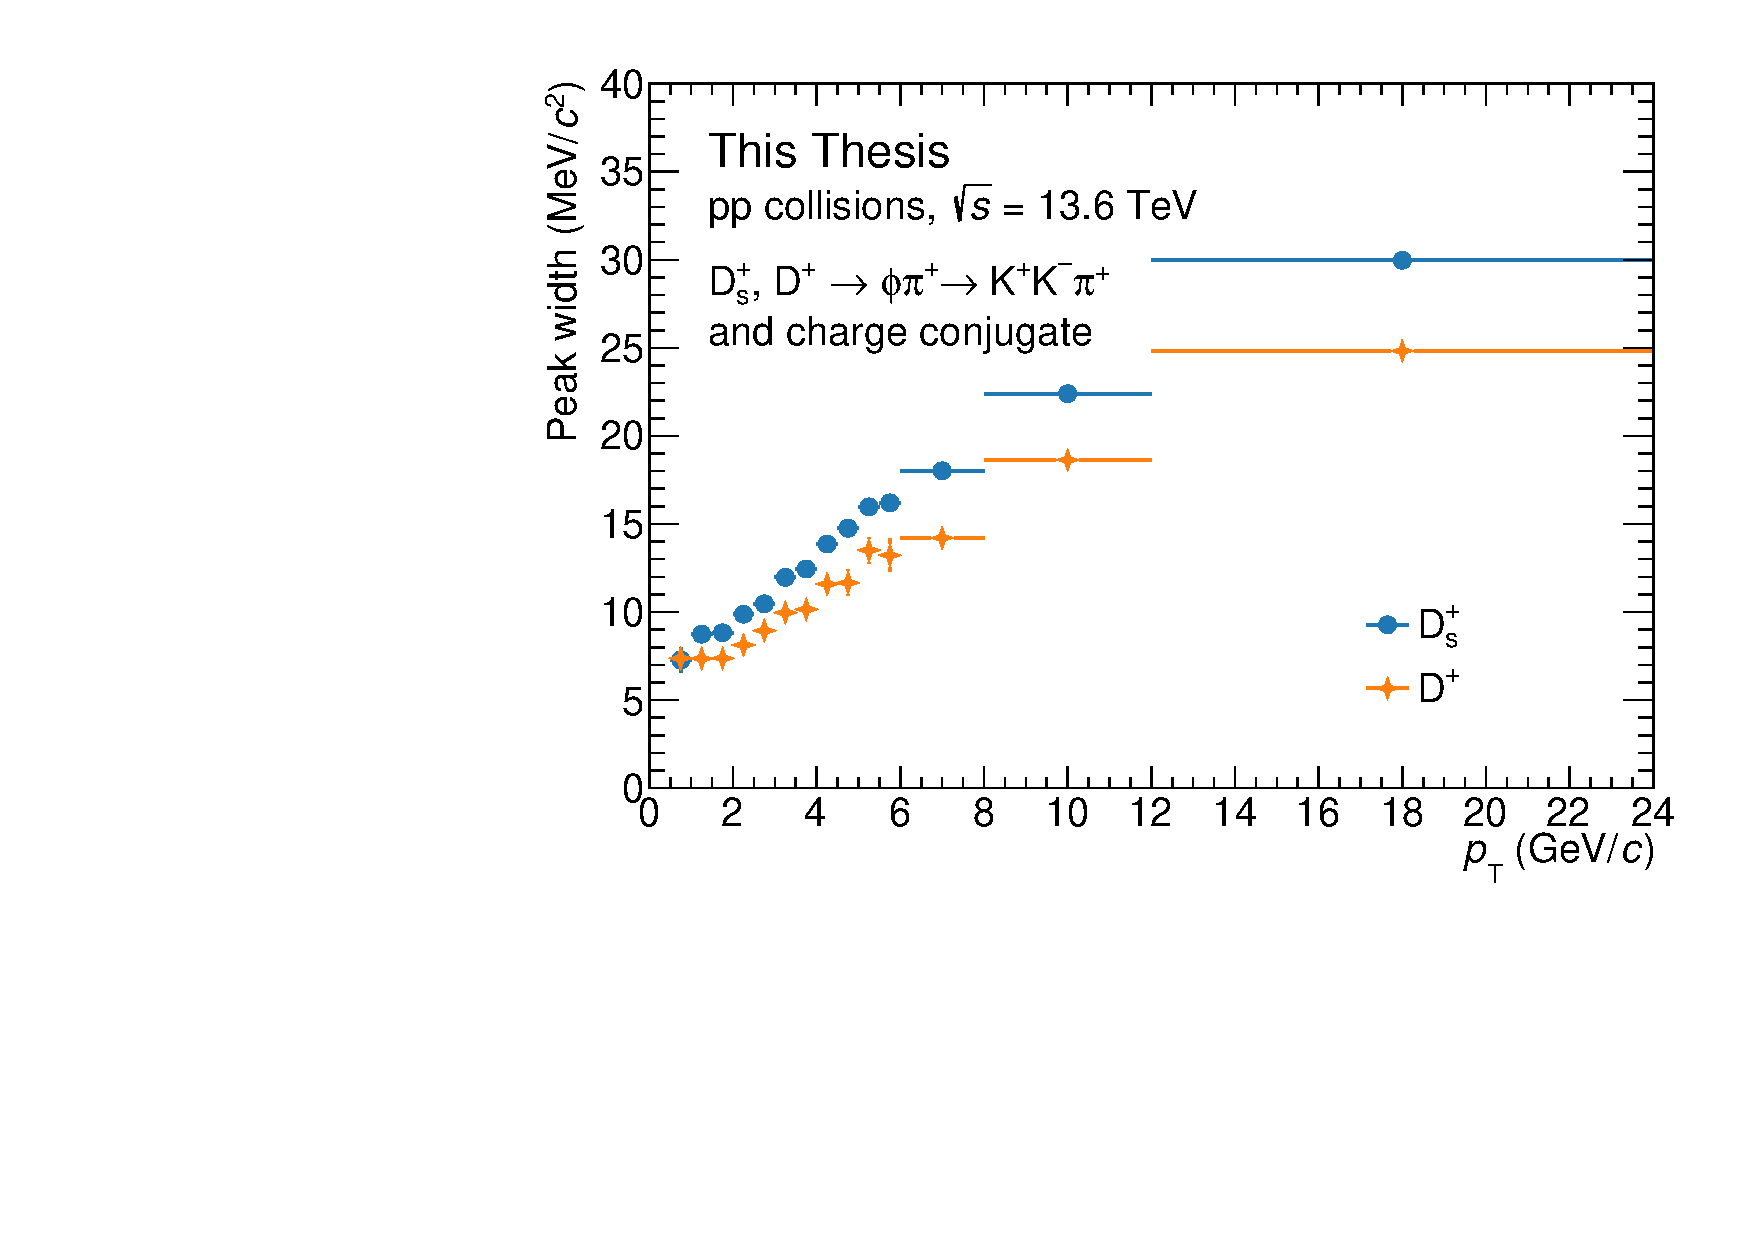
\includegraphics[width=0.48\textwidth]{Figures/Chapter 5/Sigma.pdf}
    \caption{Evolution of the mean (left panel) and width (right panel) of the Gaussian functions used to describe the \ds and \dpl meson peaks as a function of \pt. The dashed lines in the left panel represent the mass values reported in the PDG~\cite{pdg} for the two D-meson species.}
    \label{fig:mean_width}
\end{figure}

The relative contribution of the $\dpl\rightarrow\mathrm{\pi^+K^-\pi^+}$ correlated background to the total fitting function is shown in the left panel of Fig.~\ref{fig:frac_signif} as a function of \pt. At low \pt, where the PID is more effective, the contribution of the correlated background is observed to be smaller. It then increases up to 2~\gevc and then decreases due to the kinematic properties of the decay as expected from Fig.~\ref{fig:DplusSimulations}. Some residual contribution is observed at higher \pt, related to fluctuations in the fitting procedure. In the right panel of Fig.~\ref{fig:frac_signif}, the statistical significance of the extracted \ds- and \dpl-meson signals is shown as a function of \pt. Due to the large combinatorial background at low \pt, the statistical significance presents a decreasing trend with decreasing \pt for $\pt\lesssim2$~\gevc, for both D mesons. The maximum statistical significance is observed in the $2.5<\pt<3.0$~\gevc interval for the \ds meson and in the $2.0<\pt<2.5$~\gevc range for the \dpl meson, where significances of 99 and 50 are reached for the two meson species, respectively. At higher \pt, the statistical significance decreases due to the smaller number of produced D mesons, and the larger peak widths of the \ds and \dpl mesons, which result in a larger background contribution in the signal region. A sudden increase in the statistical significance is observed in the $6<\pt<8$~\gevc interval, and is due to an increase of the width of the \pt interval for the signal extraction, from 0.5~\gevc to 2~\gevc, which results in a larger number of candidates available in the signal region.

\begin{figure}[htb]
    \centering
    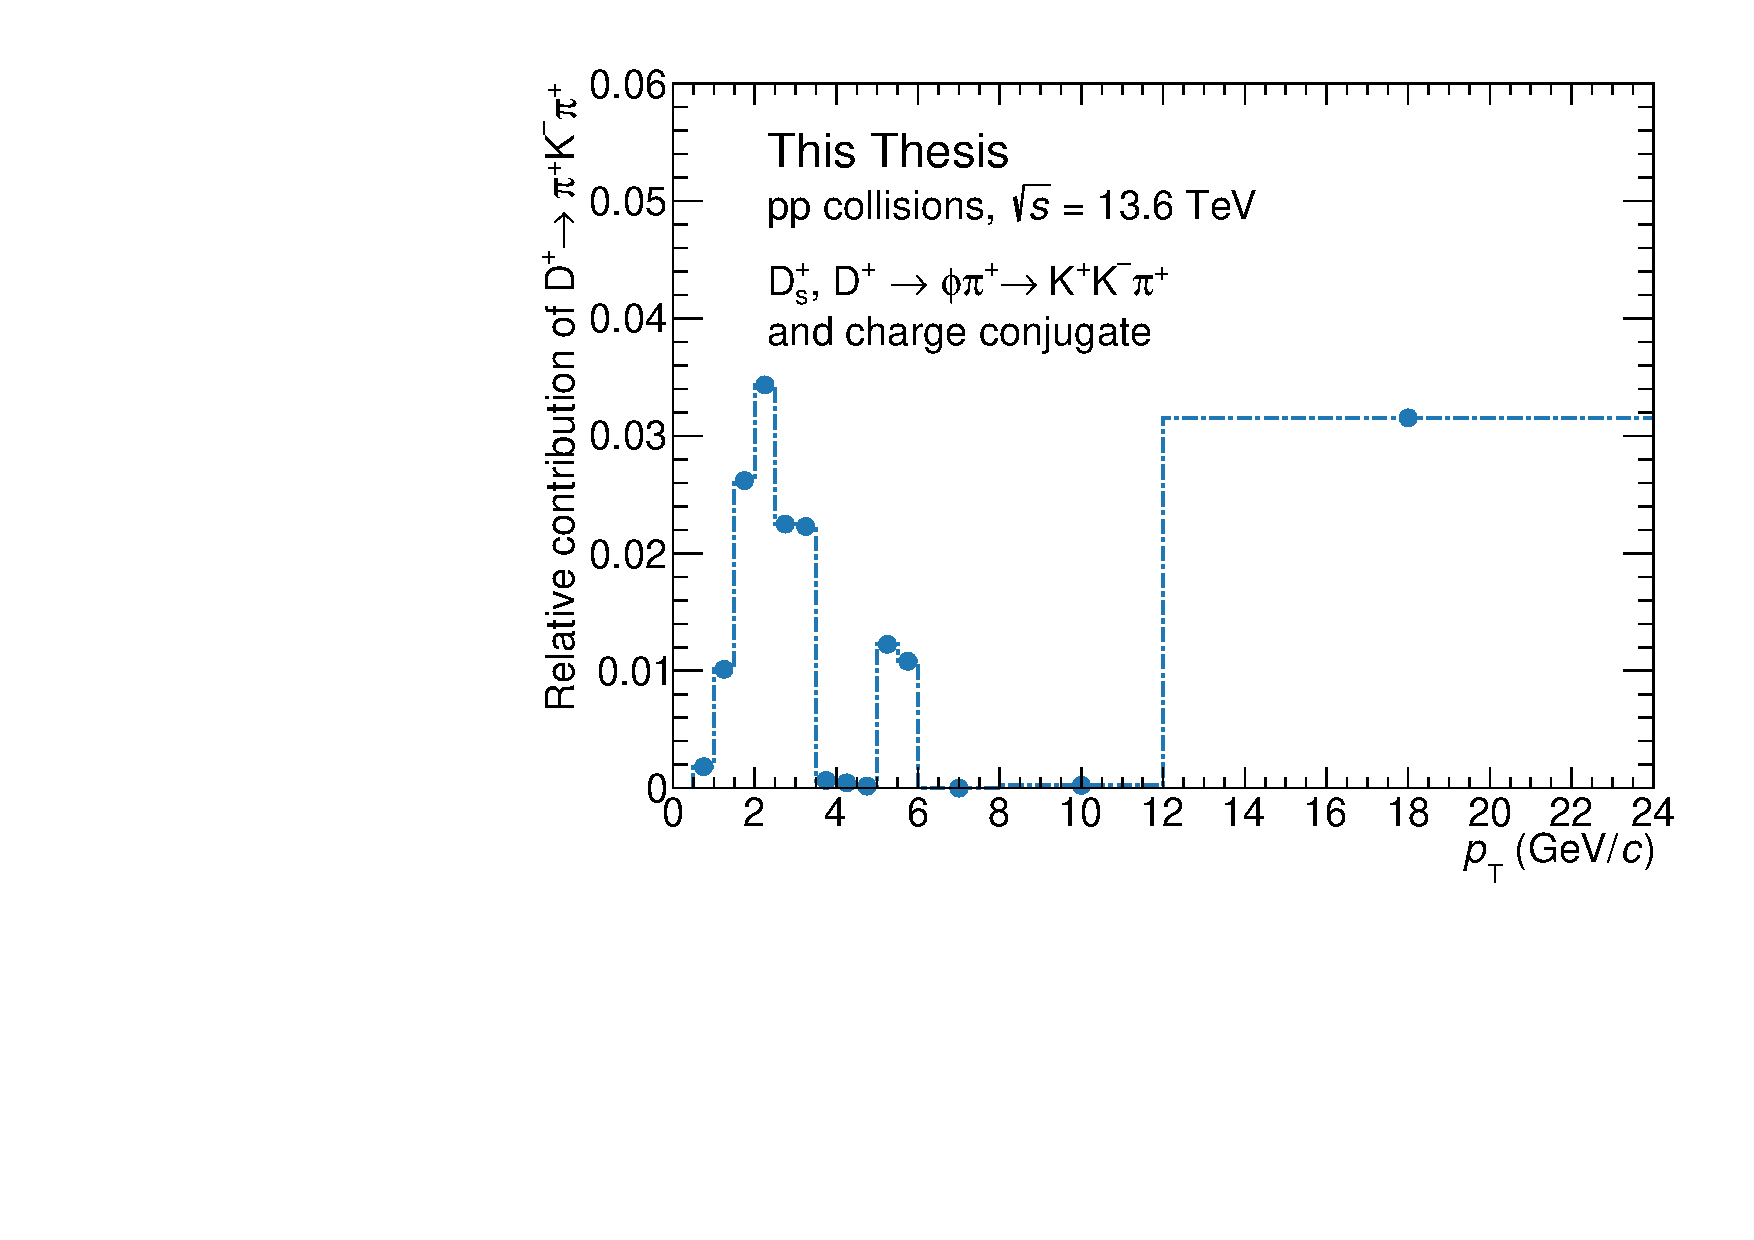
\includegraphics[width=0.48\textwidth]{Figures/Chapter 5/Frac.pdf}
    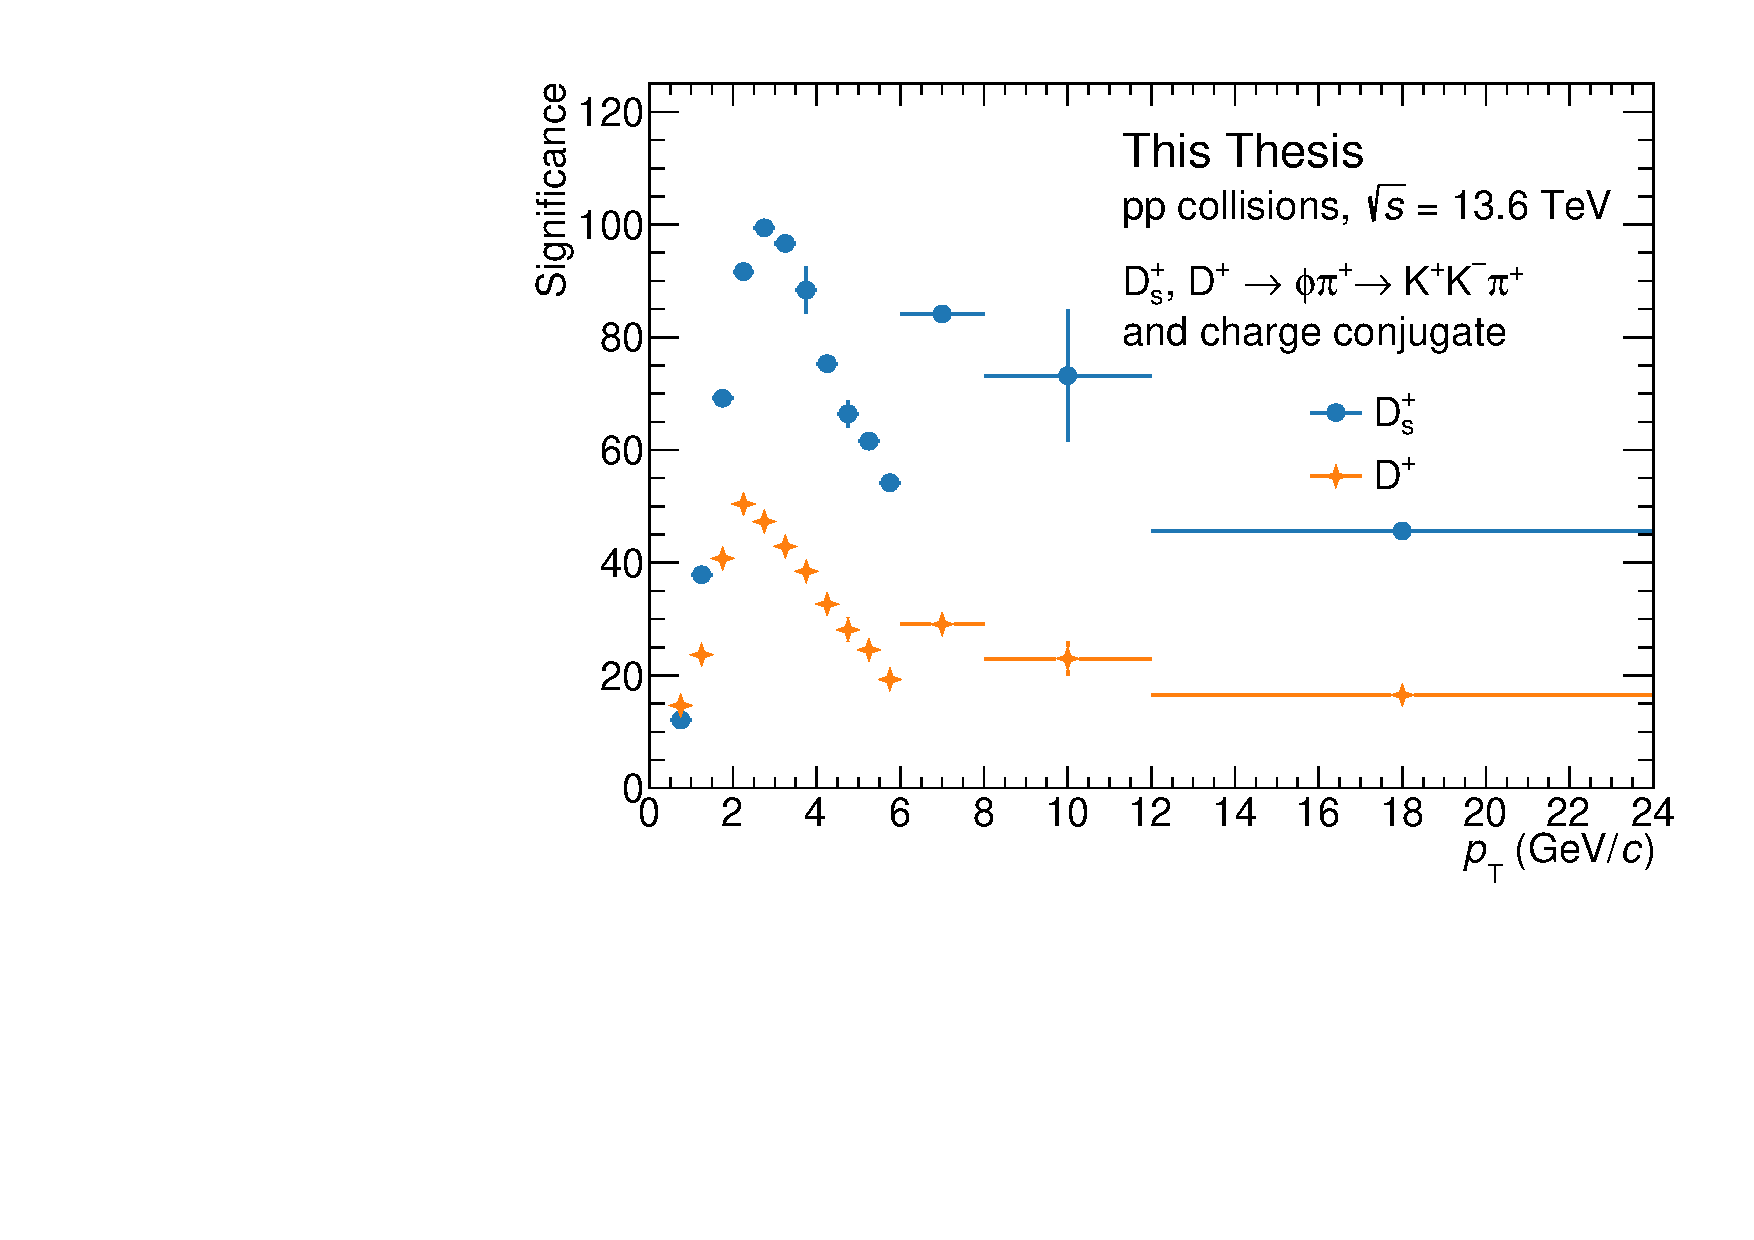
\includegraphics[width=0.48\textwidth]{Figures/Chapter 5/Significance.pdf}
    \caption{Evolution of the $\dpl \rightarrow \mathrm{\pi^+K^-\pi^+}$ relative contribution to the fitting function (left panel) and statistical significance of the extracted \ds- and \dpl-meson signal (right panel) as a function of \pt.}
    \label{fig:frac_signif}
\end{figure}



The extraction of the raw yields is affected by several arbitrary choices, for example, the functional description of the background, the choice of the fit range, the choice of fixing the \dpl width at high \pt, and the invariant-mass bin width. Changes in these choices can lead to variations in the extracted raw yields. To estimate the effect of such arbitrary choices in the final observable (the \ds/\dpl production-yield ratio), and estimate a systematic uncertainty associated with the raw yield extraction procedure, the fit is repeated several times by varying the fit range, the bin width, and the functional form of the background. In the low \pt region ($\pt<4~\gevc$), the lower fit limit is varied between 1.71 and 1.77~\gevcc, while the upper limit is varied between 2.08 and 2.14~\gevcc. The functions considered to describe the background are a second-order polynomial and an exponential function. At higher \pt (up to 8~\gevc), where the signal peaks become broader, the lower limit is varied between 1.71 and 1.75~\gevcc, while the maximum mass is varied between 2.13 and 2.19~\gevcc. The functions considered to describe the background are a second- and a third-order polynomial, as the exponential function was observed not to reproduce the background distribution. The bin width is varied between 1 and 4~\mevcc across the studied \pt interval. At $\pt>8$~\gevcc, where the \dpl-meson peak width is fixed to that of the \ds-meson divided by 1.2, the peak width of the \dpl meson is changed by varying the dividing factor by $\pm10\%$. For each possible combination of these variations, the signal is extracted for the two D-meson species, and the ratio between them is calculated. This results in 128, 96, and 288 trials for the $0.5<\pt<4$~\gevc, $4<\pt<8$~\gevc, and $8<\pt<24$~\gevc intervals, respectively. As a quality check, trials with a $\chi^2/\mathrm{ndf}$ greater than 2 are discarded. The distribution of the \ds/\dpl raw-yield ratio is then obtained for the different trials, and the mean and standard deviation are calculated. The difference $\Delta$ between the mean of this distribution and the ratio extracted with the default configuration is calculated. The systematic uncertainty is then evaluated as the sum in quadrature of the standard deviation and $\Delta$: $\sqrt{\mathrm{RMS^2}+\Delta^2}$.

\begin{figure}[htb]
    \centering
    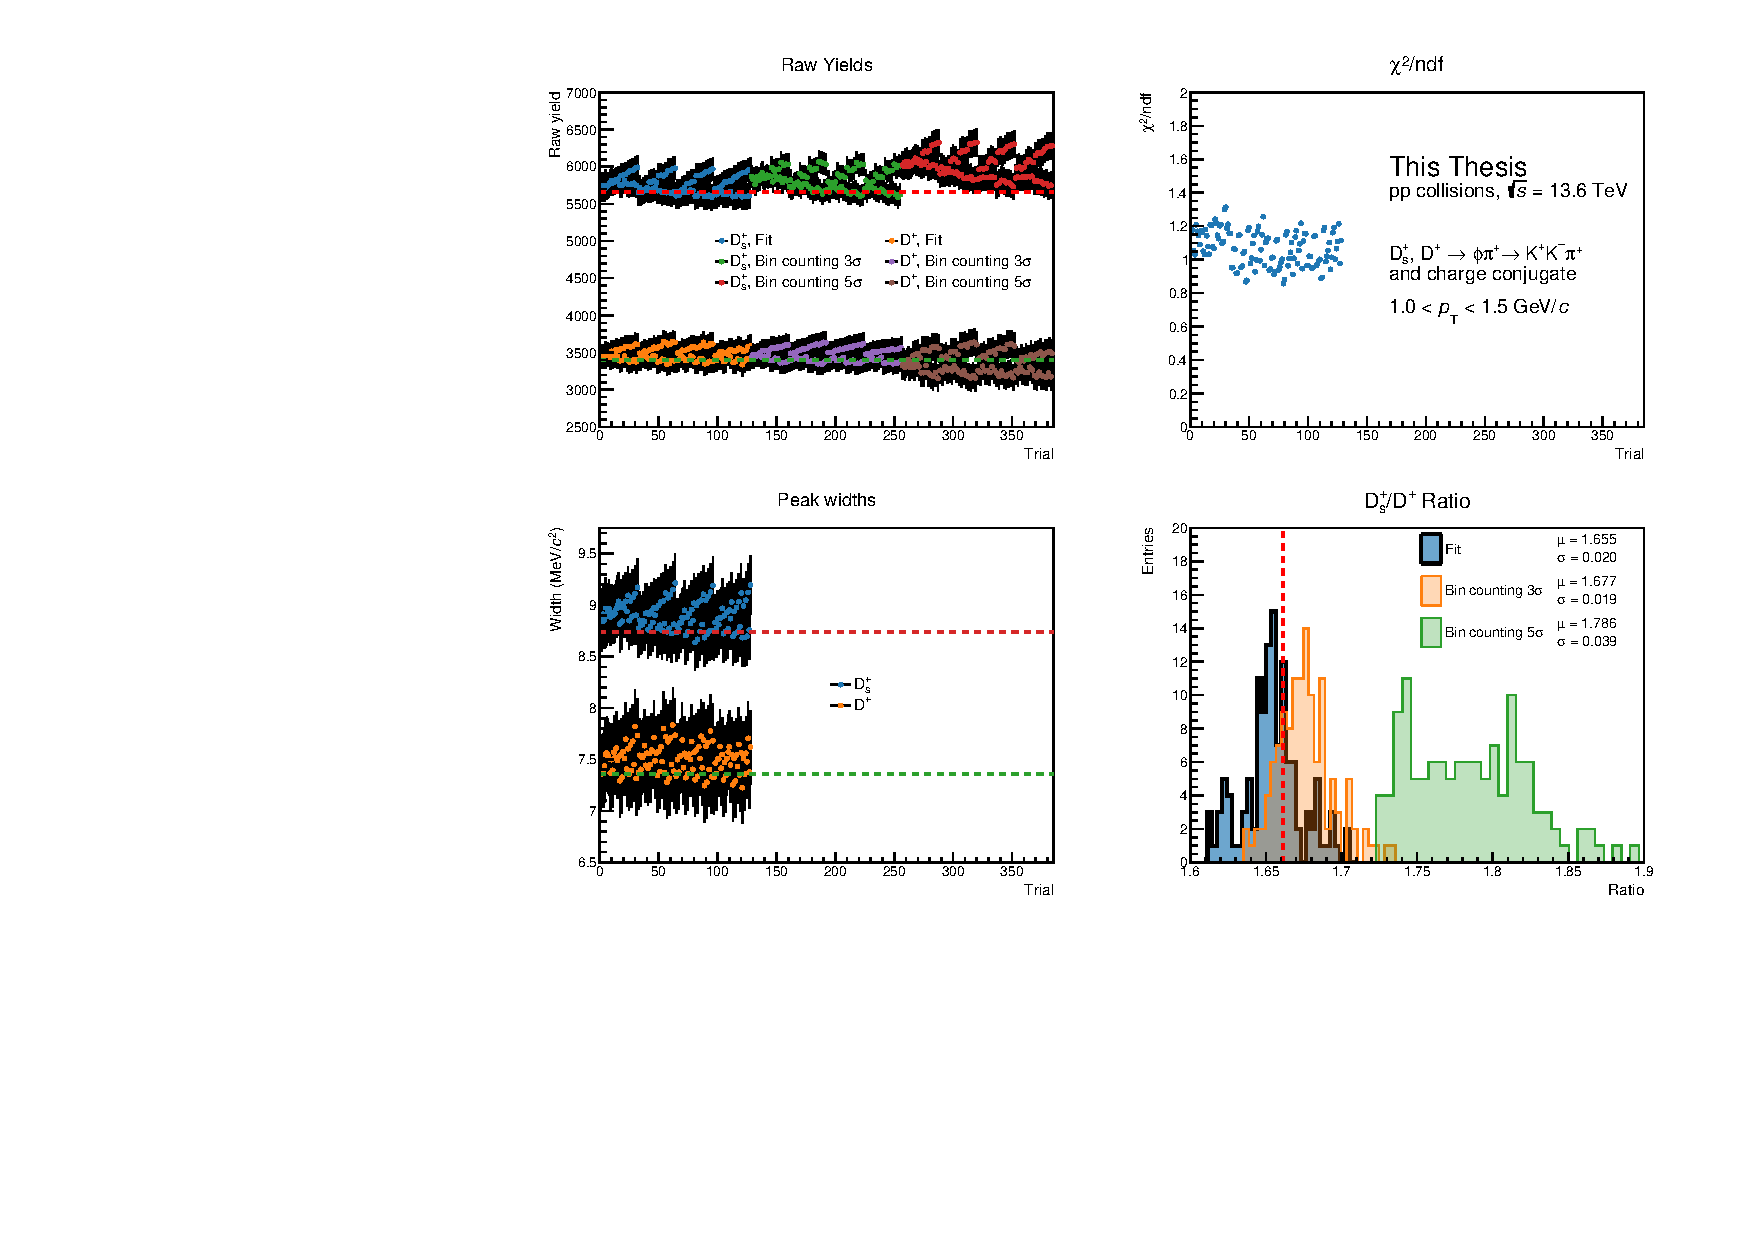
\includegraphics[width=\textwidth]{Figures/Chapter 5/RawYieldSyst.pdf}
    \caption{Results from the multi-trial approach employed for estimating the systematic uncertainty related to the raw yield extraction in the \mbox{$1.0<\pt<1.5$~\gevc} interval.}
    \label{fig:raw_yield_syst}
\end{figure}

The result of this multi-trial approach for the evaluation of the systematic on the raw-yields extraction is shown in Fig.~\ref{fig:raw_yield_syst} for the $1.0<\pt<1.5$~\gevc interval. In the top-left panel, the raw yields extracted from the fit to the invariant mass distribution are reported for the \ds and \dpl mesons for the different trials. As a cross-check, the raw yields are also extracted by summing the counts of a distribution obtained by subtracting the background fit function (composed of the function considered in the trial for the combinatorial background and of a template function for the $\dpl\rightarrow\mathrm{\pi^+K^-\pi^+}$ correlated background) from the invariant mass distribution of the candidates passing the ML selections. The bin contents are summed within 3 standard deviations from the peak mean. The extracted raw yields are stable within uncertainty across all the trials for the \dpl meson. For the \ds meson, the $3\sigma$ bin counting method presents higher raw yields when compared to the ones obtained by integrating the signal function. However, this is considered as related to fluctuations in the invariant mass distribution rather than a systematic shift of the raw yields due to a different definition of the observable. The raw yields extracted with the default configuration described above are shown as dashed lines. In the top-right panel, the $\chi^2/\mathrm{ndf}$ of the fit to the invariant mass distribution is shown for the different trials. Only trials where the signal is extracted by integration of the fitted signal function are shown in this panel. In this \pt interval, all the different trials present a $\chi^2/\mathrm{ndf}<2$, and no trial is rejected because of poor fit quality. However, at higher \pt a few trials do not survive the quality check on the $\chi^2/\mathrm{ndf}$, and are discarded. These results illustrate that the fit function is able to describe the data accurately, independently of the configuration of the fit parameters. In the bottom-left panel, the peak widths for \ds and \dpl mesons are reported, and present a stable behaviour across the different trials. The peak widths for the default configuration are also reported as dashed lines. The bottom-right panel shows the distribution of the \ds/\dpl raw-yield ratio for the different trials, obtained using the two methods previously introduced (namely, integration of the signal fit function and bin counting). The $3\sigma$ bin counting method presents a higher raw-yield ratio in this \pt interval when compared to the other method, because of the higher \ds-meson yields. The systematic uncertainty is defined as the sum in quadrature of the standard deviation of the distribution of \ds/\dpl raw-yield ratio obtained by integrating the signal function and the difference $\Delta$ between the default value reported with a dashed red line and the mean of this distribution. This quantity ranges from 1\% to 10\% of the central \ds/\dpl raw-yield ratio, depending on the considered \pt interval. The systematic uncertainty is then assigned after smoothing the \pt dependence of the obtained values. The assigned systematic uncertainty is reported in Table~\ref{tab:raw_yield_syst}.




\begin{table}[htb]
    \centering
    \caption{Systematic uncertainty on the raw-yield extraction for the ratio of the \ds and \dpl mesons yields.}
    \label{tab:raw_yield_syst}
    \vspace*{0.3cm}
    \resizebox{\columnwidth}{!}{%
    \begin{tabular}{c|cc}
    \toprule
         \pt (\gevc) & $\sqrt{\mathrm{RMS^2+\Delta^2}}$/(central \ds/\dpl) (\%) & Assigned systematic uncertainty (\%)\\
         \midrule
         0.5$-$1 & 4  & 3 \\
         1$-$1.5 & 1  & 3 \\
         1.5$-$2 & 2  & 3 \\
         2$-$2.5 & 3  & 3 \\
         2.5$-$3 & 3  & 3 \\
         3$-$3.5 & 3  & 3 \\
         3.5$-$4 & 3  & 3 \\
         4$-$4.5 & 6  & 5 \\
         4.5$-$5 & 7  & 5 \\
         5$-$5.5 & 3  & 5 \\
         5.5$-$6 & 5  & 5 \\
         6$-$8   & 8  & 8 \\
         8$-$12  & 9  & 9 \\
         12$-$24 & 10 & 10 \\
        \bottomrule
    \end{tabular}%
    }
\end{table}
